\chapter{Simulations of Modern Calorimeter Systems} \label{chapter:Simulations}

\section{Introduction} \label{section:simulations_introduction}

\subsection{Simulation Objective} \label{subsection:simulations_introduction_objective}
Any simulation is an approximation of a certain process. It is a model that one builds to try to understand something under investigation. It can come in various kinds with different names: virtual reality, avia simulator, computer game or be it any physics simulation. In the end, they are all trying to help model a process of interest. Therefore, the primary objective of any simulation is to model a certain process as good as this process actually is in reality.

Physics Simulations are not the exceptions - it is how Experimental High Energy Physics Experiments function. One starts out by having an objective to measure some quantity or to verify a hypothesis. Typically that means that a model already exists to provide with signatures and features to look for it. Then, a simulation of a system is built to measure physical quantities of interest and then to compare experimental results with simulated predictions. This final step is the most important part - if the simulation (model) has not been possible, one would not have something to compare results with and therefore no way to draw conclusions.

In what follows, two standalone calorimeter systems are examined: the High Granularity Calorimeter (HGC) \cite{Magnan:2017exp} and the Shashlik + Hadron Endcap system. Both detectors were considered as potential candidates for the CMS Phase 2 Upgrade. What matters most for the simulation is that these two systems present different choice of technology, in particular for the electromagnetic calorimeter part. Intrinsically, the Shashlik calorimeter has better resolution due to the scintillation process being very efficient, however the disadvantage is the introduction of the light to electric signal conversion part, which very often means that longitudinal segmentation is not possible. In turn, the electromagnetic part of the HGC, although has a less efficient silicon active material, allows to put the readout electronics directly on the calorimeter, which results in the longitudinal segmentation and profiling of the showers.

\subsection{Simulation Tools} \label{subsection:simulations_introduction_geant4}
For the purpose of simulating High Energy Physics (HEP) calorimeter systems physicists employ {\sc Geant4} \cite{Geant4-1,Geant4-2}, a software toolkit which provides an interface for building actual simulation, carrying it out and collecting the results. To be more precise, every simulation has the following features:
\begin{itemize}
    \item \textbf{Materials}. All the materials that are to be used in the simulation must be defined. All the properties of all of the chemical elements must be also defined. Important to point out, that if for instance one has a material that acts as a scintillator in a calorimeter, optical characteristics of such a material must be provided separately and can be optimized.
    \item \textbf{Geometry}. Using various geometrical primitives (cube, cone, etc...) a geometrical specification of the simulation has to be provided. Technically speaking, \textbf{Materials} $+$ \textbf{Geometry} define the physical layout of a calorimeter.
    \item \textbf{Physics}. One of the most important parts of a simulation is the ability to change the physics processes that are being used and see how that affects calorimeter's response. For instance, if there is a scintillation material that is expected to output light upon incoming radiation, then by turning off Scintillation Physics Process, the output of the calorimeter will be suppressed. In {\sc Geant4}, this is typically achieved via \textbf{Physics Lists} - that contain the specification of the most important physics processes.
    \item \textbf{Readout}. The whole idea of performing a simulation is to yield some output that you can then analyze further. For that, there are \textbf{Sensitive Detectors}, which get attached to \textbf{Geometry Volumes} and get triggered for every single step of any particle within that volume. What gets stored is up to the user to specify.
    \item \textbf{Primary Generators}. In order to start a simulation, one needs a trigger - a way to artificially inject some physics objects to interact with the rest of the virtual realm. Within the {\sc Geant4} context, this trigger is called \textbf{Primary Generator}. It can come in various forms: from simple particle guns to generating complicated decay processes.
    % A special case of the physics is the generation of a primary vertex. For instance, typically, when the performance of a calorimeter is studied, a precise control of the setup is required and it is achieved by shooting a single final state particle into the system. This procedure allows to deduce basic performance characteristics of the system under study.
    \item \textbf{Simulation Engine}. Finally, {\sc Geant4} provides an engine to carry out the simulation itself: track all the particles for each step, trigger various transitions for readout, apply the physics processes, etc...
\end{itemize}
%\section{Simulations of Calorimeters with Geant4} \label{section:simulations_geant}

\section{High Granularity Calorimeter} \label{section:simulations_hgc}

\begin{figure}[hbp]
    \centering
    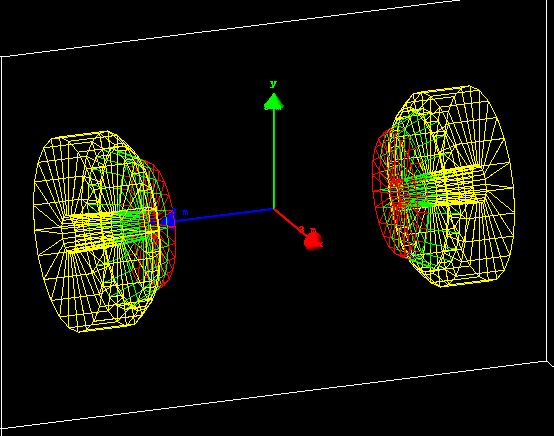
\includegraphics[width=0.9\textwidth]{figures/ch_simulations/hgc/detetor_3d/HGC_70_20.png}
    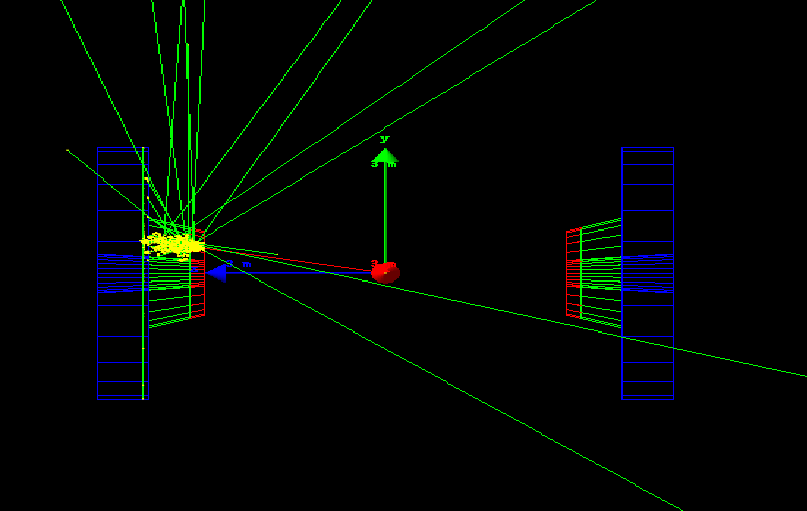
\includegraphics[width=0.9\textwidth]{figures/ch_simulations/hgc/detetor_3d/HGCal_1Event_NoSides.png}
    \caption{Full CMS Scale High Granularity Calorimeter (Top). Example of a Particle Gun response (Bottom)}
    \label{fig:simulations_hgcexamples}
 \end{figure}

\subsection{Physical Layout}
High Granularity Calorimeter consists of three parts: Electromagnetic (EM)Calorimeter, Front Hadronic (FH) and Backing (BH) Calorimeters. Both EM and FH have similar design principles: alternating layers of absorber (we use tungsten) and active materials (Silicon) mixed in together with a layer of electronics readout. Full geometry specification for the EM part can be summaried as follows:
\begin{itemize}
    \item 25 Radiation Length ($X_{0}$) Device
    \item In total 30 layers, where each layer is (absorber (W), active (Si), readout (G10/PCB)).
    \item First 10 layers have $0.5 X_{0}$ per layer
    \item Second 10 layers have $0.8 X_{0}$ per layer
    \item Third 10 layers have $1.2 X_{0}$ per layer
    \item XY-plane is subdivided into pads, with an area of each channel of 0.9 $cm^2$ for the first 20 layers and 1.8 $cm^2$ for the last 10.
\end{itemize}
Full specification for the FH part can be summarized as follows:
\begin{itemize}
    \item 4 Interaction length ($\lambda$) Device
    \item 12 layers of (absorber (W/Brass), active (Si), readout (G10/PCB)), each layer is $0.33\lambda$
    \item XY-plane is also subdivided into small pads, with each covering an area of 1.8 $cm^2$
\end{itemize}

\subsection{Detector Readout} \label{subsection:simulations_hgc_readout}
The operating principle of SiW Calorimeter is based on electron-hole pairs generated by a charged track traversing within the active material. For the purpose of simulation, we assume a constant number of such holes per 1 um step (80 holes/um), which is a valid assumption that has been previously used by CALICE SiW Electromagnetic Calorimeter. Equation~\ref{eq:simulation_hgc_responsePerCell} summarizes the computation of the response for a single pad per event.

\begin{center}
    \begin{equation}
        \label{eq:simulation_hgc_responsePerCell}
        {R(cell)} = {\sum_{n=1}^{steps} \frac{80\times \Delta x}{1um}}
 %       \caption{Response per cell. $\Delta$x is a single step size}
   \end{equation}
\end{center}

\subsection{Simulation}
The goal of our modeling is to establish the performance characteristics of our calorimeter system: response linearity and energy resolution. For that we use an electron Particle Gun with varying energies. Each event corresponds to shooting a single $e^-$ of a certain energy, performing all the tracking for all of the shower particles and recording all of the results as discussed in section~\ref{subsection:simulations_hgc_readout}. It is important to point out that each primary particle enters the detector at an angle of normal incidence for the purpose of precise control of simulation environment. Figure~\ref{fig:higgs_simulations_hgc_scatter60} provides and example of a shower distribution for a single event.

\begin{figure}[hbp]
    \centering
    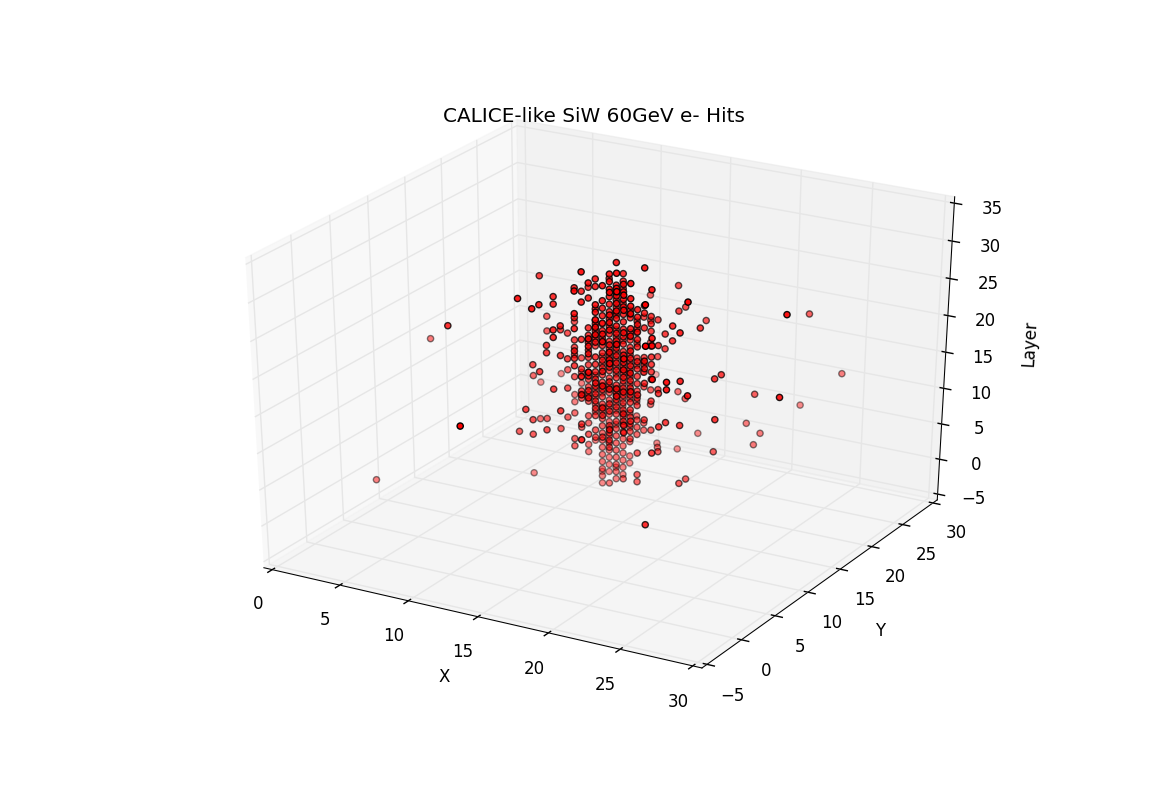
\includegraphics[width=0.9\textwidth]{figures/ch_simulations/hgc/scatter_3d/scatter_3D_60GeV.png}
    \caption{An example of a shower distribution within HGC for an incident 60 GeV $e^-$}
    \label{fig:simulations_hgc_scatter60}
 \end{figure}

\subsection{Analysis}
The objective of the readout analysis is to establish calorimeter performance characteristics: linearity of response and energy resolution. Not all systems are linear and intrinsically SiW-calorimeters are not linear in response. The reason for desirability of this characteristic is the ability to easily calibrate the device. In other words, given a linear system - the conversion of the raw response to energy is trivially established. In summary, the following steps are to be followed to etablish the performance characteristics:

\begin{itemize}
    \item Compute Total Response. In the case of SiW, we used right-hand side of equation~\ref{eq:simulations_hgc_totalResponse} to relate energy and total response.
    \item Overlay particle gun energy with total response as in Figure~\ref{fig:simulations_hgc_pblinearityresolution}. Perform a linear fit and extract the calibration coefficient.
    \item Using the derived calibration coefficient, compute the reconstructed energy distributions.
    \item Compute and overlay Resolution (according to equation~\ref{eq:simulations_hgc_resolution}) with incident energy. Perform the fit using equation~\ref{eq:simulations_hgc_resolutionfitfunc}.
\end{itemize}

\begin{center}
    \begin{equation}
        \label{eq:simulations_hgc_totalResponse}
         {E} = {CC} \times {Raw Response}. = {CC} \times {\sum_{i=1}^{n_{layers}} w_i \times  R_{i}}
    \end{equation}
\end{center}{}

\begin{center}
    \begin{equation}
        \label{eq:simulations_hgc_resolution}
         {Resolution} = {\frac{\mu_E}{\sigma_E}}
    \end{equation}
\end{center}

\begin{center}
    \begin{equation}
        \label{eq:simulations_hgc_resolutionfitfunc}
         {f(x)} = {\sqrt{\frac{\alpha^2}{x^2} + C^2}}
    \end{equation}
\end{center}

\subsection{Results}
Exercising the procedure described just above, we first obtain reconstructed energy distributions in figures~\ref{fig:simulations_hgc_pbenergyreco} and ~\ref{fig:simulations_hgc_wenergyreco}.

 \begin{figure}[hbp]
    \centering
    \includegraphics[width=0.95\textwidth]{figures/ch_simulations/hgc/performance/Pb/EnergyRECO.png}
    \caption{Reconstructed Energy Distributions with Lead Absorber.}
    \label{fig:simulations_hgc_pbenergyreco}
 \end{figure}

  \begin{figure}[hbp]
    \centering
    \includegraphics[width=0.95\textwidth]{figures/ch_simulations/hgc/performance/W/EnergyRECO.png}
    \caption{Reconstructed Energy Distributions with Tungsten Absorber.}
    \label{fig:simulations_hgc_wenergyreco}
 \end{figure}

A guassian fit is performed, resolution is computed and provided in figures~\ref{fig:simulations_hgc_pblinearityresolution} and ~\ref{fig:simulations_hgc_wlinearityresolution}.
 \begin{figure}[hbp]
    \centering
    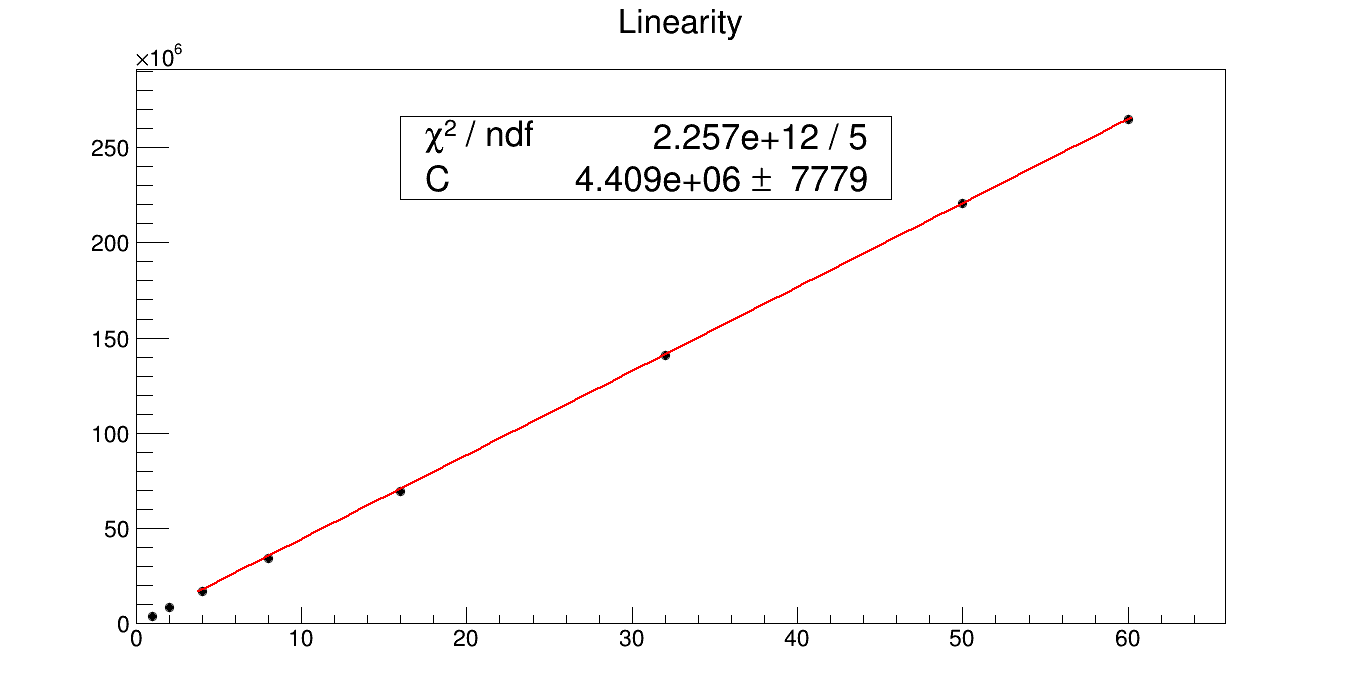
\includegraphics[width=0.9\textwidth]{figures/ch_simulations/hgc/performance/Pb/Linearity.png}
    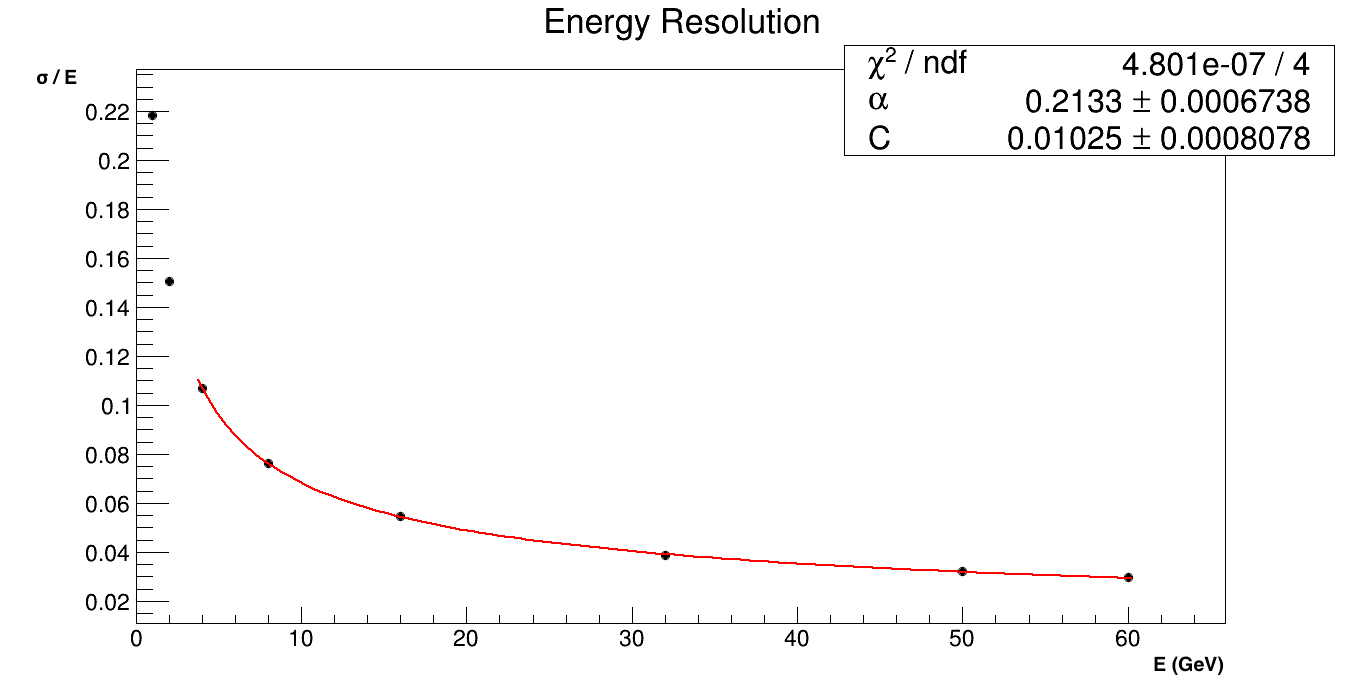
\includegraphics[width=0.9\textwidth]{figures/ch_simulations/hgc/performance/Pb/Resolution.png}
    \caption{Linearity (Top) and Energy Resolution (Bottom)}
    \label{fig:simulations_hgc_pblinearityresolution}
 \end{figure}

 \begin{figure}[hbp]
    \centering
    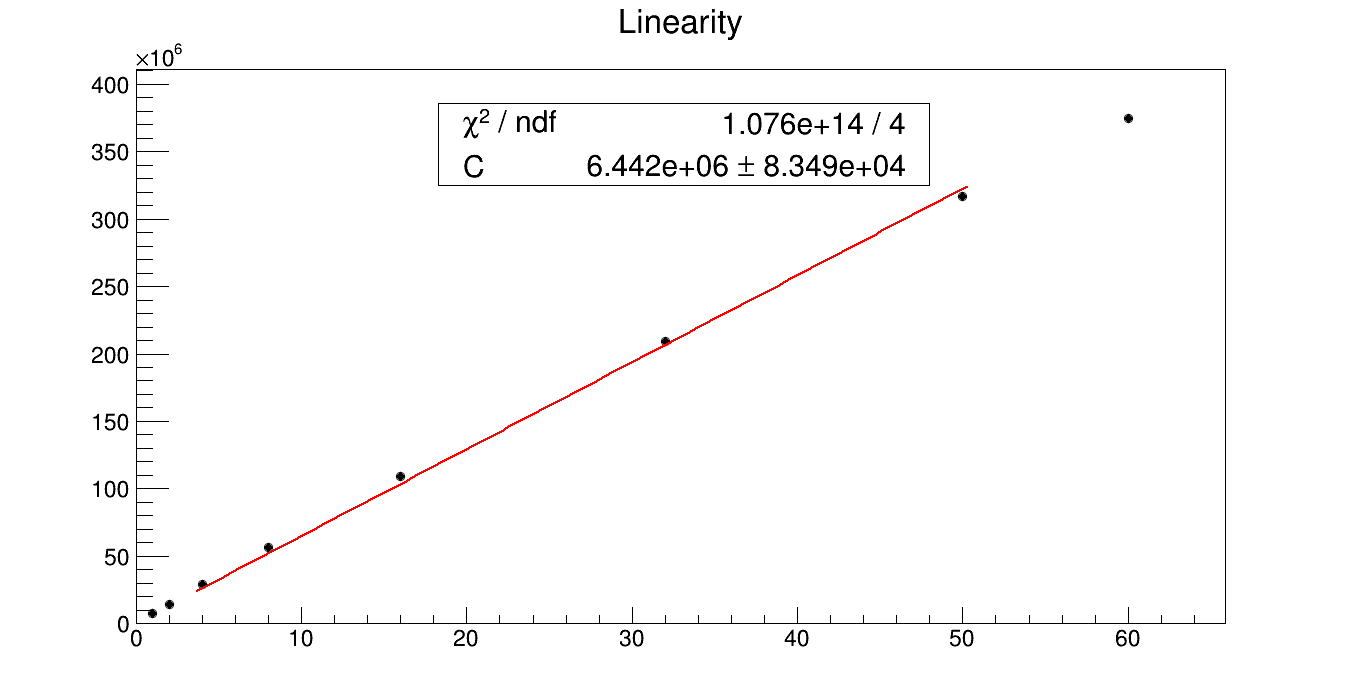
\includegraphics[width=0.9\textwidth]{figures/ch_simulations/hgc/performance/W/Linearity.png}
    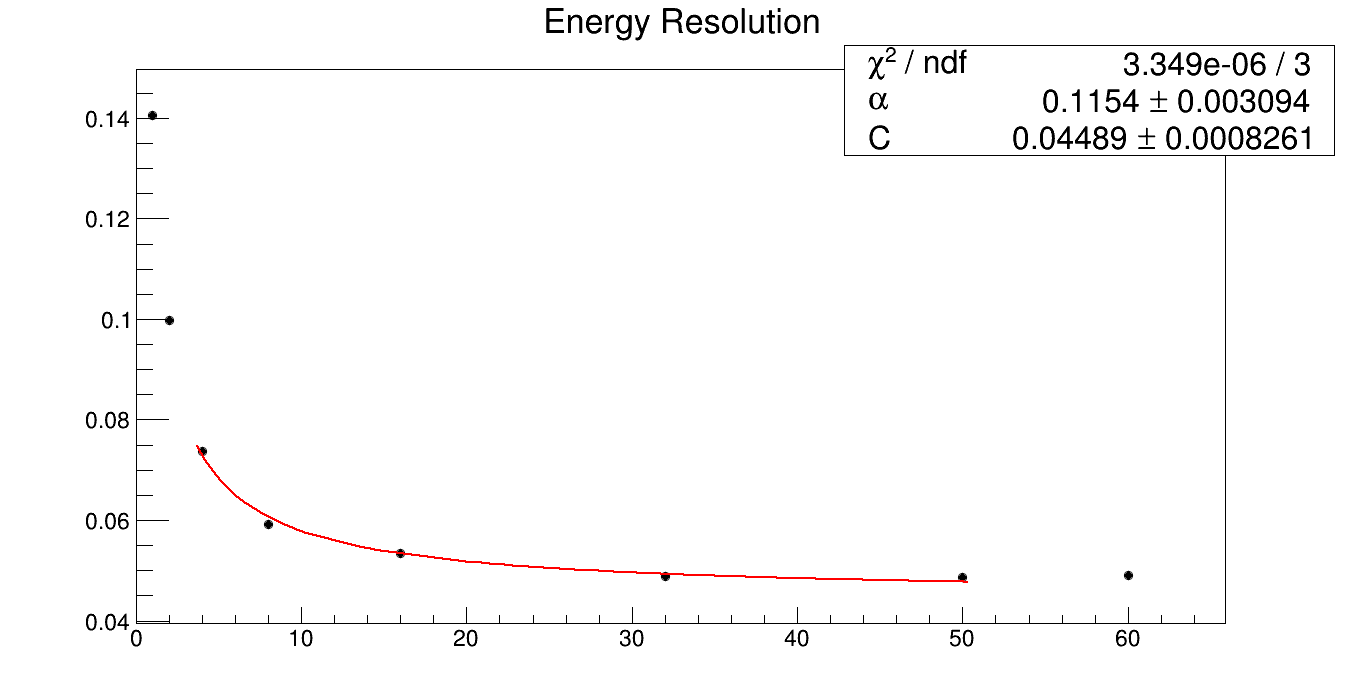
\includegraphics[width=0.9\textwidth]{figures/ch_simulations/hgc/performance/W/Resolution.png}
    \caption{Linearity (Top) and Energy Resolution (Bottom)}
    \label{fig:simulations_hgc_wlinearityresolution}
 \end{figure}
\section{Shashlik + Hadron Endcap} \label{section:simulations_shashlik}
\begin{figure}[htbp]
    \centering
    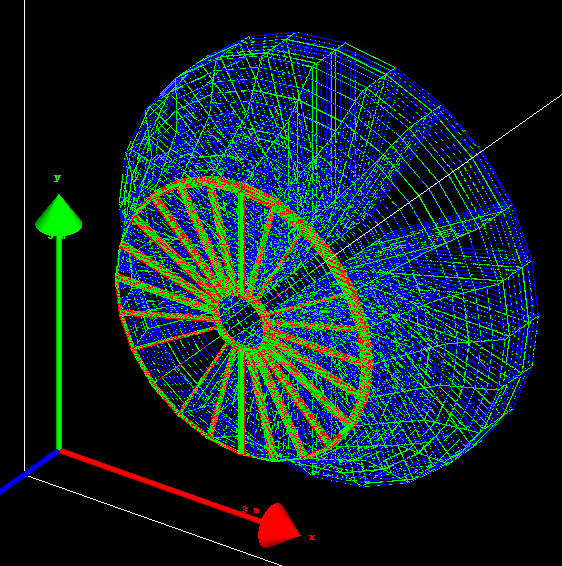
\includegraphics[width=0.9\textwidth]{figures/ch_simulations/shashlik/geometry/Shashlik+HE_Complete_Wire.png}\\
    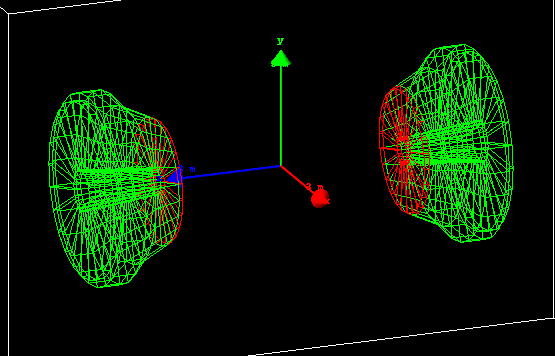
\includegraphics[width=0.9\textwidth]{figures/ch_simulations/shashlik/geometry/SHE_70_20.png}
    \caption{Full CMS Scale Shashlik + HE System (from different angles)}
    \label{fig:higgs_simulations_shashlikexamples}
 \end{figure}

\subsection{Physical Layout}
Shashlik is an Electromagnetic Calorimeter System with the name implicitly reflecting its structure and the choice of readout technology. The physical layout is similar to HGC~\ref{section:simulations_hgc}: alternating layers of absorber and active materials, however there is no electronics unit sitting on the calorimeter itself. Instead, wave-length shifting fibers go through the whole length of the calorimeter and are responsible for light capture and transmission to the electroncs unit for conversion into analog signal. Full specification of the Shashlik Calorimeter can be summarized as follows:
\begin{itemize}
    \item 25-30 $X_0$ device
    \item No Longitudinal Segmentation
    \item Alternating layers of absorber (tungsten W) and active (LYSO) materials.
    \item Active Material used is LYSO plastic scintillator.
\end{itemize}
Hadron Endcap (HE) is an active CMS Endcap Calorimeter that is part of the HCAL subsystem. Design principles are similar with respect to Shashlik, however has a slightly different choice of readout technology \cite{Baiatian:2008zz}. Calorimeter specification can be summarized as follows:
\begin{itemize}
    \item $10\lambda$ device
    \item Alternating layers of absorber (Brass) and active (SCSN-81 plastic scintillator) materials
    \item Partial Longitudinal segmentation.
\end{itemize}

\subsection{Detector Readout}
For the purpose of simplification, in the simulation the assumption is made to have a perfect light capture and transmission for both Shashlik and Endcap. Also no modeling of the wave-length shifting fibers or any kind of photodetectors. In other words, looking for upper limits of our calorimeter performance. The metric of the system's response is defined to be the number of generated photons within the scintillator. Scintillation mechanics is responsible for light generation and \textbf{G4Scintillation}, \cite{geant4}, physics process of {\sc Geant4} provides these capabilities via \textbf{optical photons}. For the purpose of modeling, {\sc Geant4} defines two different types of photons: regular photons, that obey the laws of quantum physics, and optical photons, that follow the laws of geometrical optics. Optical photons do not participate in the conservation of energy laws and do not deposit any energy into the scintillator (this fact allows for optimizations).

\subsection{Parametrized Detector Readout}
Typical light yields for a scintillator are in thoughsands of optical photons per MeV of deposited energy into the scintillation material. The exact number is material-dependent and varies substantially. Given that the input particle has energies in the GeV range, the number of optical photons that gets generated goes well above 1 M. Tracing all of these photons is a complicated and time-consuming task for Geant's engine. Moreover, given that \textbf{optical photons} can not deposit energy into the material, one can simply \textbf{count and kill} them right after they've been generated. Therefore, for the purpose of optimizing the time it takes to generate a single event, the parametrization of the response of a schintillator is performed. This procedure allows to substantially speed up the simulation without degrading the performance.

\subsection{Analysis and Results}
The analysis procedure is identical to the one described for HGC in section~\ref{section:simulations_hgc} and will not be repeat here. There are 2 main differences: first, the readout metric here is defined to be simply the total number of generated optical photons. No weighting layer by layer applied for neither Shashlik nor HE. And second, HE is calibrated separately, by shooting pions with a different set of energies. Figure \ref{fig:simulations_shashlik_linearity} shows the results of computing the linearity for both Shashlik and HE. It is clear, especially comparing to {\sc HGC}, that Shashlik exhibits better linearity properties.
 \begin{figure}[htbp]
    \centering
    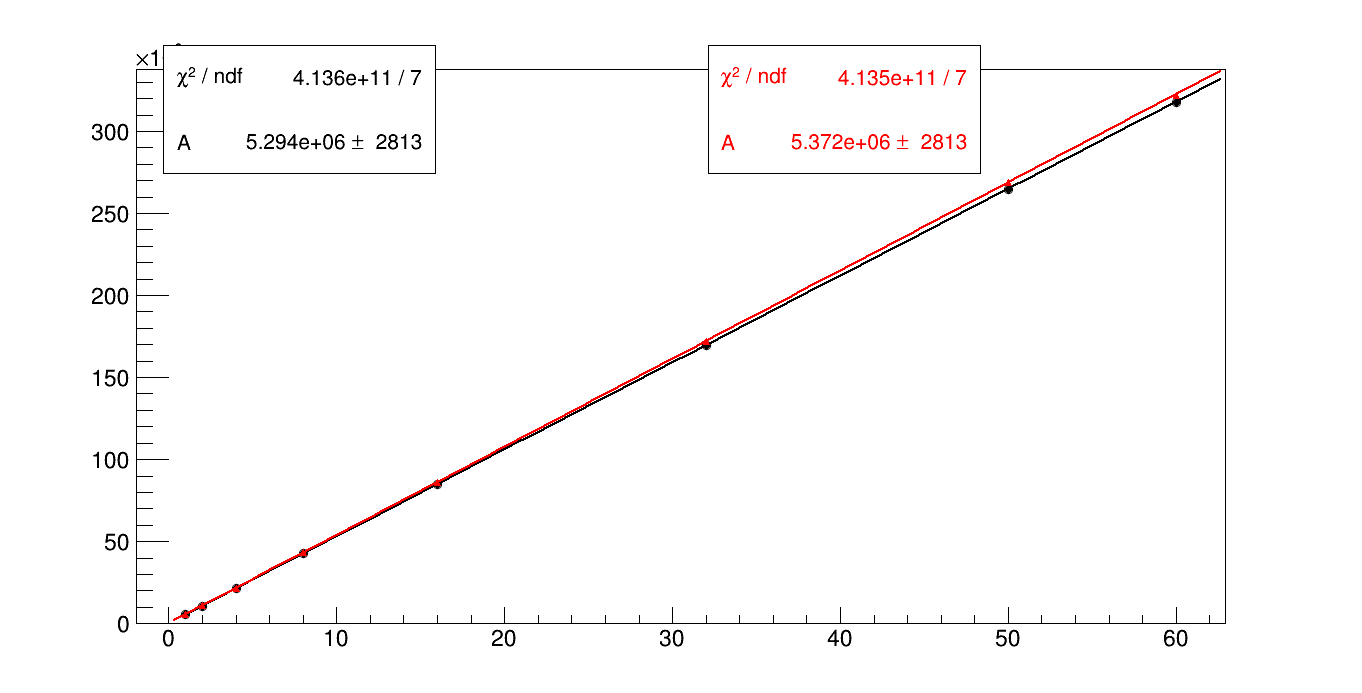
\includegraphics[width=0.95\textwidth]{figures/ch_simulations/shashlik/performance/ResponseVsEnergy.png}\\
    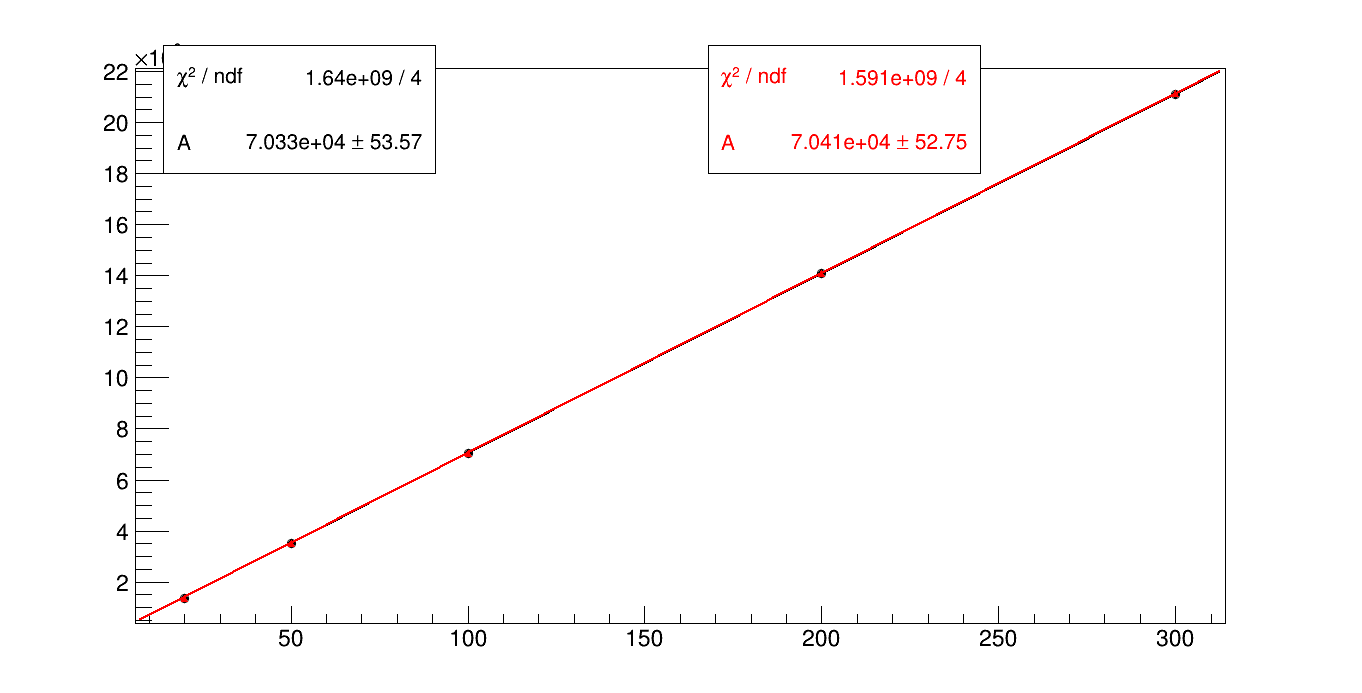
\includegraphics[width=0.95\textwidth]{figures/ch_simulations/he/performance/Linearity.png}
    \caption{Shashlik's Linearity (Top) and Hadron Endcap Linearity (Bottom)}
    \label{fig:simulations_shashlik_linearity}
 \end{figure}

Figures \ref{fig:simulations_shashlik_energyreco}, \ref{fig:simulations_he_energyreco} shows the reconstructed energy distributions for Shashlik and HE, respectively. Shashlik and HE are calibrated separately as they constitute isolated parts of the system. Note this is different with repsect to HGC, where calibration of EM and FH parts was done together.
\begin{figure}[hbtp]
    \centering
    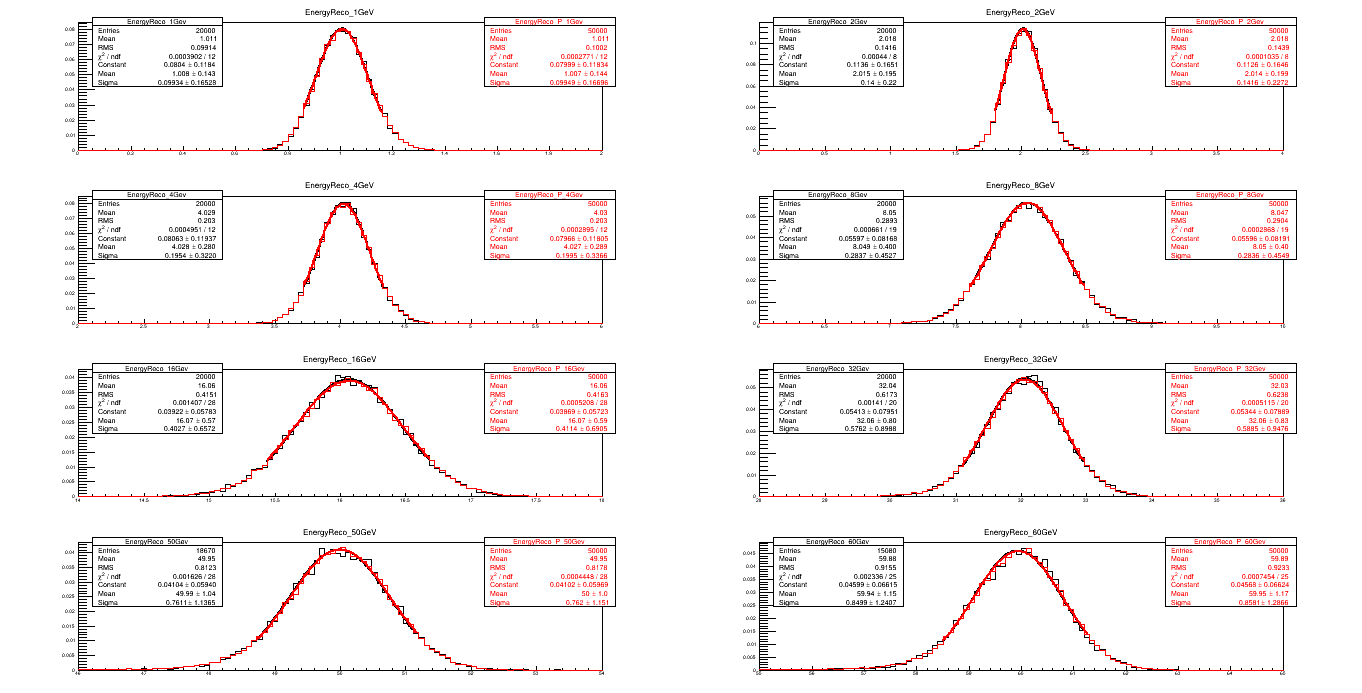
\includegraphics[width=0.95\textwidth]{figures/ch_simulations/shashlik/performance/EnergyRecoDistributions.png}
    \caption{Reconstructed Energy Distributions for Shashlik}
    \label{fig:simulations_shashlik_energyreco}
 \end{figure}
 \begin{figure}[hbtp]
    \centering
    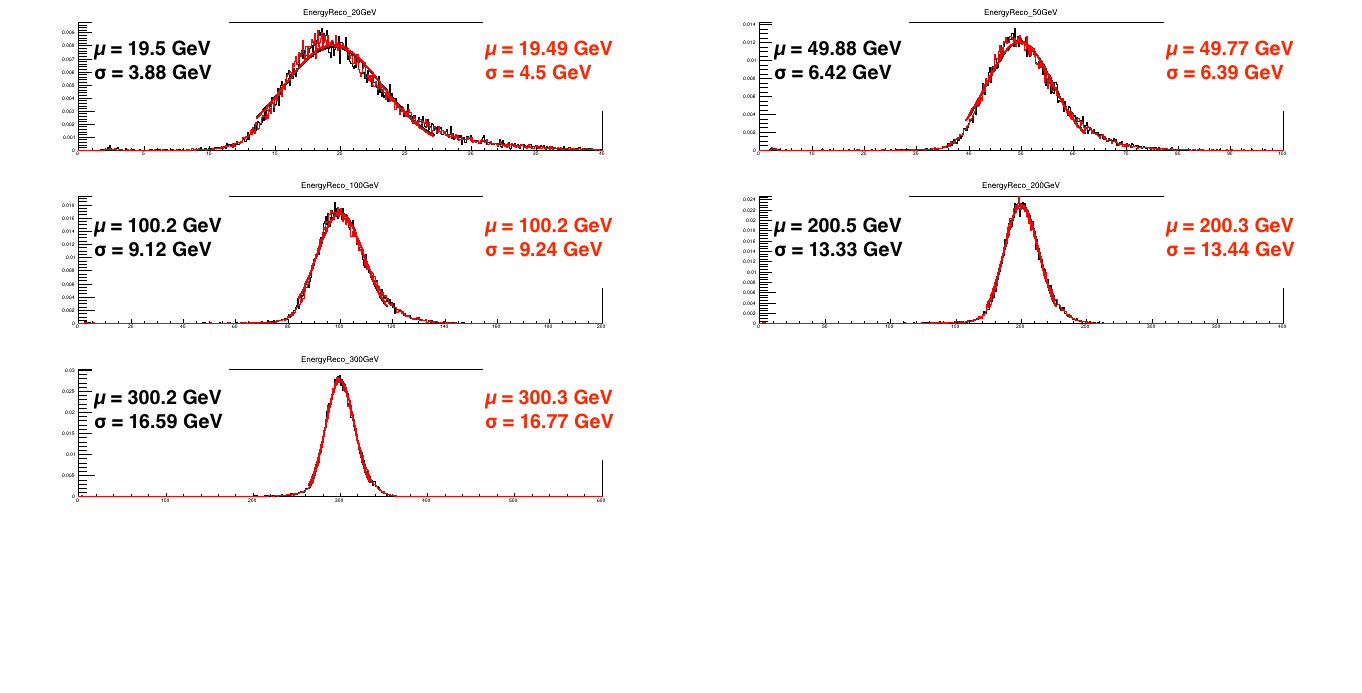
\includegraphics[width=0.95\textwidth]{figures/ch_simulations/he/performance/EnergyRECODistributions.png}
    \caption{Reconstructed Energy Distributions for Hadron Endcap}
    \label{fig:simulations_he_energyreco}
 \end{figure}

 Results for the energy resolution are provided in figures \ref{fig:simulations_shashlikhe_resolution}. The differences between the parametrized response and the use of optical photons is negligible.
 \begin{figure}[htbp]
    \centering
    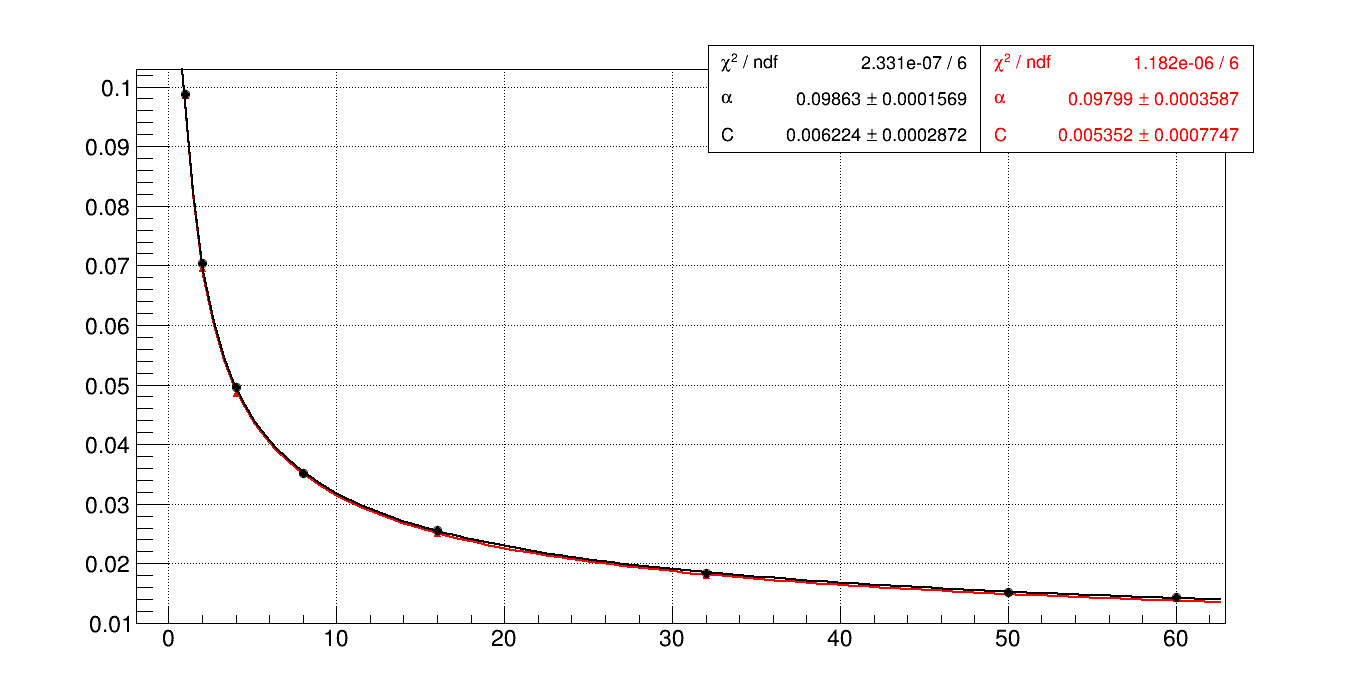
\includegraphics[width=0.95\textwidth]{figures/ch_simulations/shashlik/performance/energyResolution.png}\\
    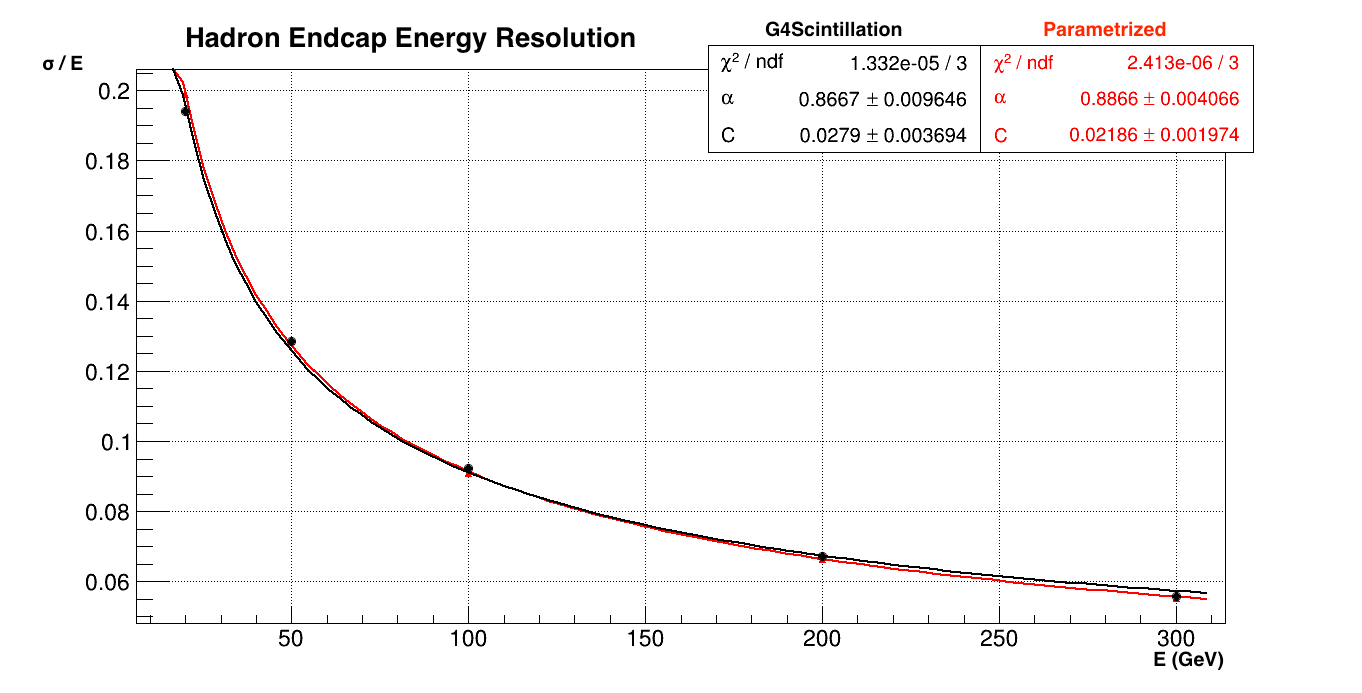
\includegraphics[width=0.95\textwidth]{figures/ch_simulations/he/performance/Resolution.png}
    \caption{Energy Resolution Shashlik (Top) and Hadron Endcap (Bottom)}
    \label{fig:simulations_shashlikhe_resolution}
 \end{figure}
%\section{Toy CMS} \label{section:simulations_scaleup}

\subsection{HGC}

\subsection{Shashlik + Hadron Endcap}
\section{Conclusions} \label{section:simulations_conclusions}
Simulations of two standalone systems have been built: High Granularity Calorimeter (CALICE SiW) and Shashlik/HE System. Baseline performance (Linearity and Energy Resolution) has been established. %Finally we scaled both systems up to the production CMS dimensions and evaluated the reconstruction efficiency.

Standalone Simulations of Calorimeters is an ideal playground for optimizing the parameters of future systems. It avoids unneccessary overhead, which is always introduced once you try to scale things up and use very precise simulations like CMS. The time to physics gets substantially reduced and allows to accelerate the development of reconstruction techniques. A very interesting future use case is the Machine Learning (ML) Benchmarking. In comparison, Mnist Digit Classification, \cite{mnist}, has become the defacto benchmarking for the field of Computer Vision and Artificial Intelligence. Energy Regression of a standalone calorimeter system could be a similar standard for the field of Calorimetry.

% % Chapter Three - A Search for a Heavy Majorana Neutrino
% \chapter{A Search for a Heavy Majorana Neutrino}\label{HMNSearch}

% This search involves the cutting edge physics surrounding neutrino mass.  For a thorough review of neutrino physics, the reader should consult \cite{nMass1, nMass2, nMass3}.

% \section{Introduction}
% 	One of the first hints at physics \textit{beyond the Standard Model} (BTSM) is the fact that neutrinos have non-zero mass\cite{1987A, nMass4}.  The Standard Model cannot be used to explain neutrino mass, implying a lack of understanding by physicists of the mechanisms underlying mass generation for fundamental particles.

% 	The leading theoretical extension to the Standard Model which explains neutrino mass is the so-called ``seesaw" mechanism\cite{seesaw1, seesaw2, seesaw3, seesaw4}.  The seesaw mechanism posits that the smallness of the observed neutrino masses is due to the largeness of the mass of a new heavy state, $N$.  The neutrino mass, $m_\nu$, can be written in terms of the heavy Majorana neutrino (HMN) mass $M_N$:  $m_\nu \sim y^2_\nu v^2/ M_N$, where $y_\nu$ is a Yukawa coupling and $v$ is the Higgs vacuum expectation value in the Standard Model. Due to the new heavy neutrino's Majorana nature it is its own anti-particle, which allows for processes that violate lepton number conservation by two units.   As the leading candidate for explaining the smallness of the neutrino masses, experimentally searching for Majorana neutrinos is thus of fundamental importance.

% 	The production of HMNs at hadron colliders has been studied fairly extensively \cite{Maj_hadCol_1, Maj_hadCol_2, Maj_hadCol_3, Maj_hadCol_4, Maj_hadCol_5}, with interest renewed by the inauguration of the Large Hadron Collider \cite{NoteTAO, NOTEATLAS, NOTETao2}.

% 	This search, as well as those at previous colliders (LEP, LHC2011), uses a model-independent phenomenological approach, assuming that the HMN mass, $M_N$, and $V_{\ell N}$, (the mixing element describing the mixing between the heavy Majorana neutrino and the SM neutrino $\nu_\ell$ of flavor $\ell$), are free parameters.

% 	Previous direct searches for heavy Majorana neutrinos have been reported by the DELPHI\cite{delphi} and L3\cite{l3} collaborations. These searches set limits on the mixing element squared\footnote{The mixing element squared is directly proportional to the HMN production cross section.}  for Majorana neutrino masses below $\sim$90 GeV/$c^2$. More recently, the CMS\cite{CMS_NR_2011} and ATLAS Collaborations~\cite{ATLAS_NR_2011} have performed direct searches and set limits on $|V_{e N}|^2$ for masses up to $\sim$200 GeV/$c^2$ and on $|V_{\mu N}|^2$ for masses up to $\sim$300 GeV/$c^2$.

% 	The analysis described in this thesis is a detailed search for the resonance production of the HMN at the LHC with the CMS detector using the 2012 data set with an integrated luminosity of $19.7$~fb$^{-1}$.  The search is for events with same sign muons and two jets in the final state.  The Feynman diagram for this process is shown in Figure \ref{fig:feyDiagram}.  An important motivation for this search is that Standard Model processes creating this signature are very small, as will be detailed in Section \ref{bkg}.

% 	That being said, there are still Standard Model processes that can contribute to what is called `background' that have to be understood, including so-called ``fake muon'' processes in which muons that aren't a product of the signal process might be mistaken for muons that are.

% 	Throughout this analysis, muons are referred to as either `prompt', or `non-prompt'.  Prompt muons are muons that can be traced back to the primary vertex, (where the collision took place), and satisfy all of our muon selection criteria.  Generally, prompt muons originate from the decay of a W or Z boson, or the hypothesized HMN signal.  The largest prompt contamination background is from Standard Model diboson production ($WW$, $ZZ$), where the bosons decay directly to muons.

% 	Non-prompt muons are muons that originate from jets, and can be real muons generated via the decay of a b-quark or so-called decays-in-flight, or jets mis-identified as a muon, each with the potential to contaminate the signal region.

% 	Figure~\ref{fig:HMNXSec} shows the cross section for HMN production and decay via the process in Figure \ref{fig:feyDiagram} as a function of Majorana neutrino mass for $| V_{\ell N}|^2 = 1.0$. The plot shows the results at leading order from del~Aguila et al.~\cite{NOTEATLAS} for $\sqrt{s} = 7$ TeV and 8 TeV.

% 	This analysis has 5 parts:  Designing selection criteria to maximize signal and minimize background; estimating backgrounds; validating selection and background on control datasets; comparing predictions with data; and interpreting results.

% 	%%%%%%%%%%%%%%%%%%%%%%%%%%%%%%%%%%% Feynman Diagram + Xsec %%%%%%%%%%%%%%%%%%%%%%%%%%%%%%%%%%%%%%%%
% 	\begin{figure}
% 		\begin{centering}
% 			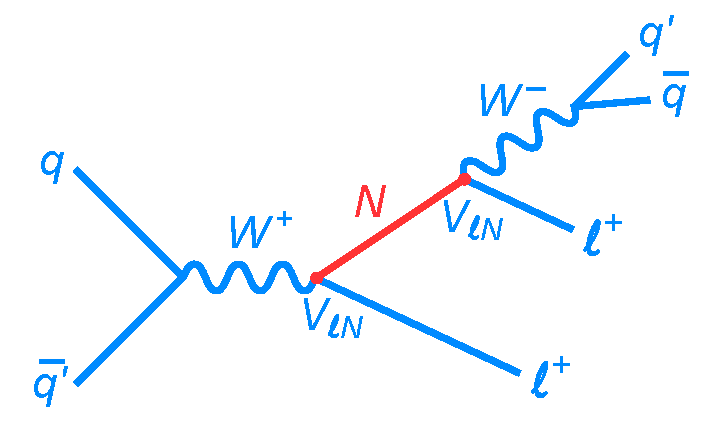
\includegraphics[scale=0.75]{figures/Ch_3_Introduction/FeyDiagram.pdf}
% 		\par\end{centering}
% 		\caption[A Feynman diagram for resonance production of a Majorana Neutrino (N) in hadron colliders.]{\label{fig:feyDiagram} A Feynman diagram for resonance production of a Majorana neutrino (N) in hadron colliders.}
% 	\end{figure}

% 	\begin{figure}
% 		\begin{centering}
% 			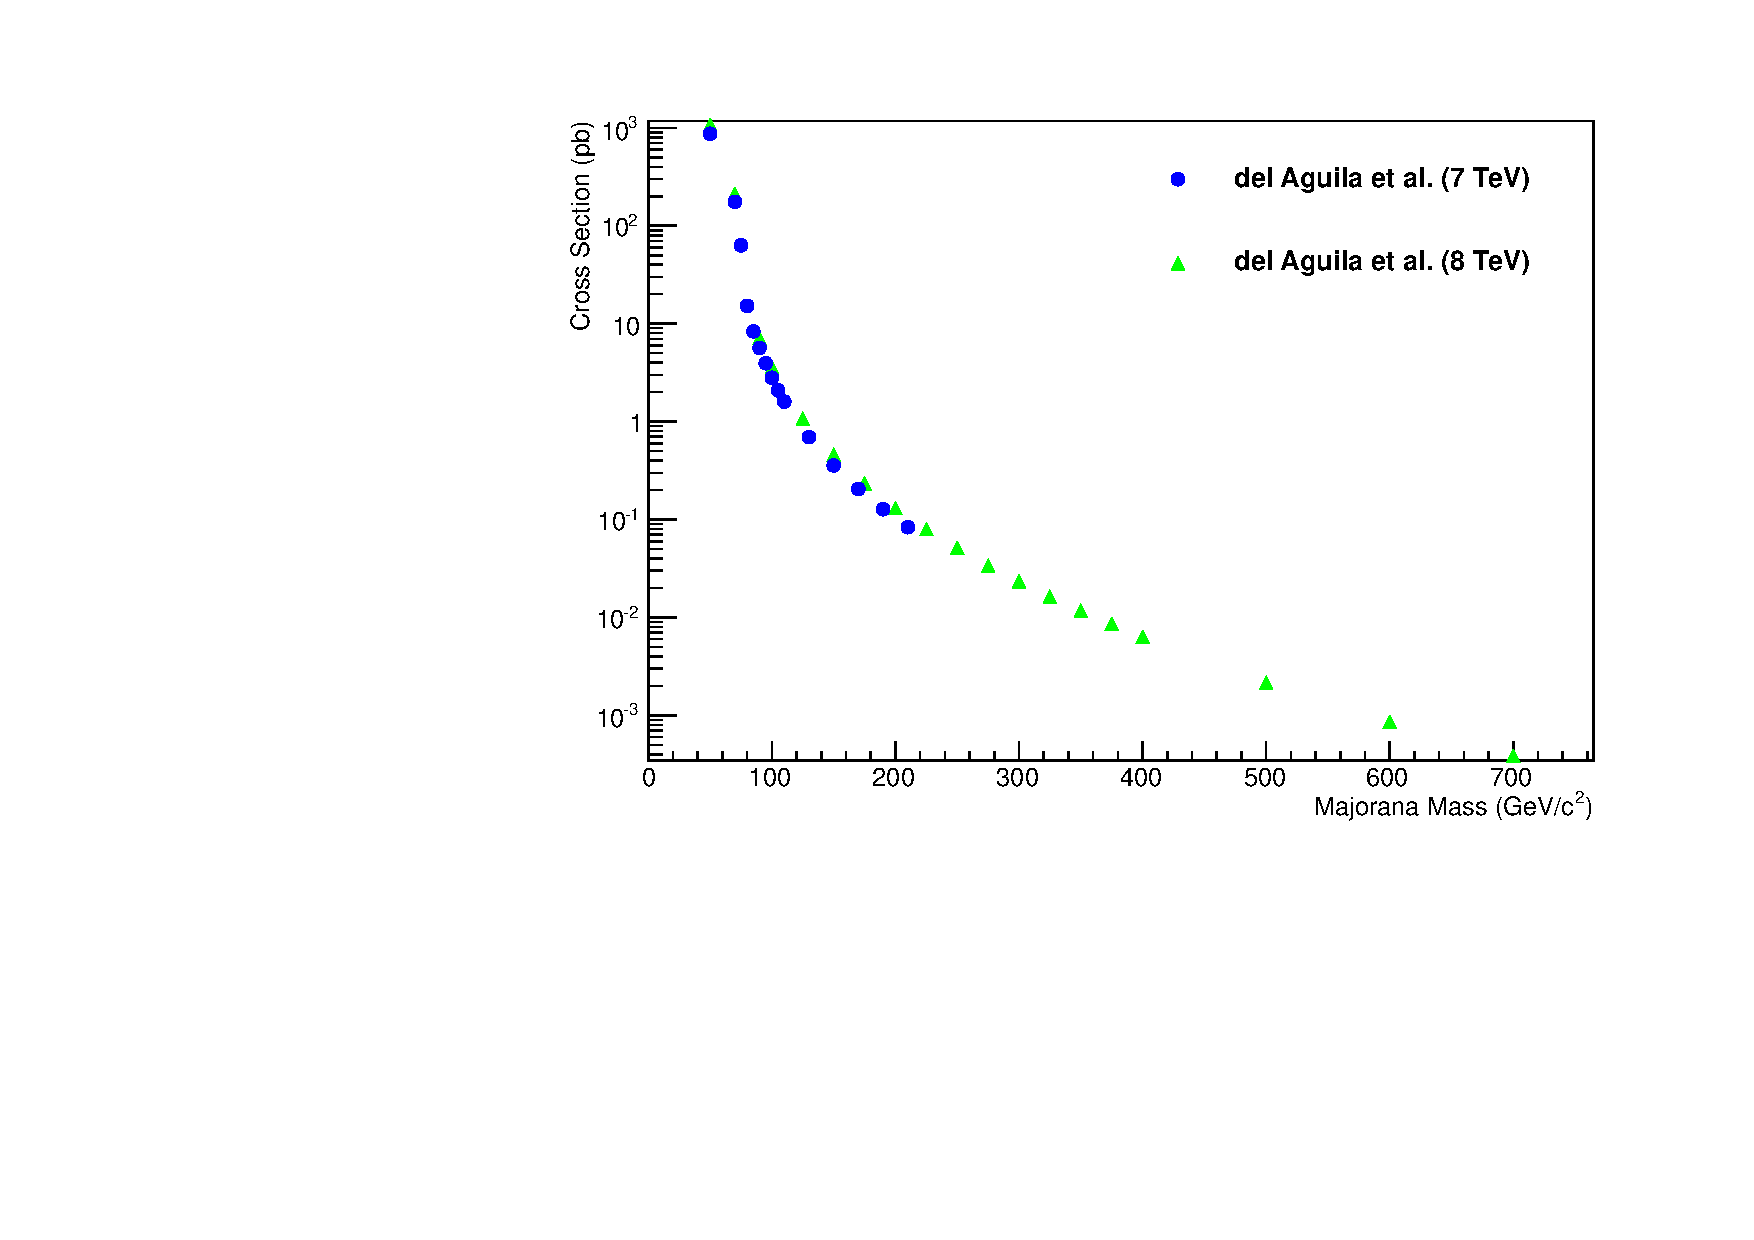
\includegraphics[scale=0.75]{figures/Ch_3_Introduction/majorana_xs_8TeV.pdf}
% 		\par\end{centering}
% 		\caption[Cross sections for resonance production of a Majorana neutrino as a function of Majorana neutrino mass.]{\label{fig:HMNXSec} Cross sections for resonance production of a Majorana neutrino as a function of Majorana neutrino mass. \cite{aguila}}.
% 	\end{figure}
% 	%%%%%%%%%%%%%%%%%%%%%%%%%%%%%%%%%%%%%%%%%%%%%%%%%%%%%%%%%%%%%%%%%%%%%%%%%%%%%%%%%%%%%%%%%

% \section{Monte Carlo Event Generation}
% 	Monte Carlo (MC) event generators have been developed to assist physicists in designing analyses by simulating the decays and kinematics of a physical process, as well as how the signal they are searching for may show up in the real CMS detector.  Two groups of MC datasets were used in this analysis: one group for signal, the other for background.  The datasets used for background studies are referred to as \textit{Standard Model MC samples}, whereas signal MC samples are referred to as, simply, \textit{signal} datasets.

% 	There are two steps to the generation process:
% 	\begin{itemize}
% 		\item Generation of the event and its decay process
% 		\item	Simulation of the detector response
% 	\end{itemize}
% 	\bigskip


% 	The three main software packages used by this analysis to generate, hadronize, and simulate the signal and background MC datasets are the ALPGEN, Pythia, and GEANT4 software packages, described below.

% 	\subsection{Signal Event Generation}
% 		Event generation for the HMN signal was done using the software package ALPGEN \cite{alpgen}.  The production and decay process was implemented in ALPGEN to leading order (LO) as described in \cite{NOTEATLAS}.  The produced datasets were simulated at a collision energy of 8 TeV, with the parton distribution function (PDF) set CTEQ6M used.  The output was stored in \textit{Les Houches} 1.0 format, (see Reference \cite{LHA} for a description of the format), and supplied to the CMS Data Operations group for official MC production.

% 		After generation, the events are hadronized using Pythia\cite{Pythia} version 6.4 to generate events for each HMN mass.  Once the events are generated, they must be simulated along with detector quirks like electronic noise or gaps in coverage in order to understand how the particles will be reconstructed by the detector.

% 		The official production signal MC samples along with their LO cross sections as a function of HMN mass are shown in Table \ref{table:sig_MC}, with abbreviations used listed in Table \ref{table:MCabbreviations}.  These samples were generated using an HMN-muon coupling value of $S_{\mu\mu} = |V_{\mu N}|^2 = 1$.

% 		This does not include next-to-leading order (NLO) calculations, though a multiplicative $k$-factor of 1.34 is applied to account for higher order corrections.  This is based on the $k$-factors calculated for $W'$ production with the NNLO calculation as in FEWZ\footnote{FEWZ is a software package for hadronic Z production, short for \textit{Fully Exclusive W, Z Production through NNLO in pQCD}.} \cite{FEWZ1, FEWZ2, CMS_Wp_kfac}.


% 	\subsection{Simulation}
% 		Detector simulation of the generated events occurs after the generated events are interfaced with a specific CMSSW version, as each CMSSW version differs in how it simulates the detector response and reconstructs the simulated events.  The generated event datasets for this analysis were interfaced with CMSSW\_5\_3\_12\_patch2, where parton showering, vertex smearing, GEANT4\cite{Geant4} detector simulation, digitization of the millions of simulated electronics signals, and particle reconstruction were performed.  The MC samples are reweighted to ensure the proper simulation of the number of interactions per beam crossing, based on previous LHC operation history.

% 		An entire software model of the CMS detector was developed using GEANT4 in order to effectively simulate the CMS detector response.  Referred to as ``Full Simulation" (FullSim), each particle in an event is simulated step by step through the detector, a process called \textit{tracking}, (not to be confused with the tracker subdetector).  Each step considers a number of detector properties including the physics of the decay process and the generation of secondary particles radiated by the effects of the magnetic field on the particles, or showers created by interactions of the particle with detector materials.


% 	\subsection{Standard Model Monte Carlo Samples}
% 		Monte Carlo datasets produced for background estimation are listed in Table \ref{table:SM_MC}, with the abbreviations used listed in Table \ref{table:MCabbreviations}.  The Standard Model backgrounds included were diboson production, $t\bar{t}W$ production, same sign $W$ production via double $W$-strahlung and double parton scattering.  The $t\bar{t}$, $W$+jets, and QCD samples are used to validate the `fake background' estimation method, described in Section \ref{bkg}.  Each sample is reweighted to ensure proper simulation of the number of interactions per crossing due to pileup.

% 		A list of the signal MC datasets used in this analysis can be found in Table \ref{table:sig_MC}, with the abbreviations used in the table found in Table \ref{table:MCabbreviations}.



% 	%%%%%%%%%%%%%%%%%%%%%%%%%%%%%%%%%% MC Datasets Used %%%%%%%%%%%%%%%%%%%%%%%%%%%%%%%
% 	\begin{table}
% 		\caption{Summary of Standard Model Monte Carlo datasets used.}
% 		\label{table:SM_MC}
% 		\begin{center}
% 			\begin{tabular}{ l  l  c  c }
% 			\hline
% 			Dataset  				&  Dataset Name 										& \(\sigma(pb)\) 		&  $\int {\cal L} dt$ (pb$^{-1}$)\\
% 			\hline
% 			% diboson
% 			$W^+W^-$ 			& {\tt /WW\_TZ\_8TeV\_pythia6\_TA/S12a} 					& 54.8 				& $1.82 \times 10^5$\\
% 			$WZ$ 				& {\tt /WZ\_TZ\_8TeV\_pythia6\_TA/S12a} 					& 33.2 				& $3.01 \times 10^5$\\
% 			$ZZ$ 				& {\tt /ZZ\_TZ\_8TeV\_pythia6\_TA/S12a} 						& 17.7 				& $5.55 \times 10^5$\\
% 			$W\gamma$ 			& {\tt /WGToLNuG\_TZ-MG-TA/S12a} 						& 462 				& $1.04 \times 10^4$\\
% 			$W^{+}W^{+}$ 			& {\tt /WpWpqq\_8TeV-MG/S12a} 							& 0.248 				& $4.03 \times 10^5$\\
% 			$W^{-}W^{-}$ 			& {\tt /WmWmqq\_8TeV-MG/S12a} 							& 0.0888 				& $1.08 \times 10^6$\\
% 			dp~$W^{\pm}W^{\pm}$ 	& {\tt /WW\_DoubleScattering\_8TeV-PY/S12a} 				& 0.588 				& $  1.42  \times 10^6$\\

% 			%triboson
% 			$WW\gamma$			& {\tt /WWGJets\_8TeV-MG\_v2/S12a} 						& 0.528 				& $5.76 \times 10^5$\\
% 			$WWW$ 				& {\tt /WWWJets\_8TeV-MG/S12a}							& 0.082				& $2.68 \times 10^6$\\
% 			$WWZ$ 				& {\tt /WWZNoGstarJets\_8TeV-MG/S12a} 					& 0.058  				& $3.83 \times 10^6$\\
% 			$WZZ$ 				& {\tt /WZZNoGstarJets\_8TeV-MG/S12b} 						& 0.0197  				& $1.12 \times 10^7$\\
% 			$ZZZ$ 				& {\tt /ZZZNoGstarJets\_8TeV-MG/S12a} 						& $5.53 \times 10^{-3}$ 	& $4.07 \times 10^7$\\

% 			% top
% 			$t \bar t$ 				& {\tt /TTJets\_MBD\_TZ\_8TeV-MG-TA/S12b} 					&  234 				& $2.96\times 10^4$\\
% 			%
% 			$t$~($t W^-$) 			& {\tt /T\_tW-CH-DR\_TZ-powheg-TA/S12a} 					& 10.7 				& $4.65 \times 10^4$\\
% 			$\bar t$~($\bar t W^+$) 	& {\tt /Tbar\_tW-CH-DR\_TZ-powheg-TA/S12a} 				& 10.7 				& $4.61 \times 10^4$\\
% 			$t$~($s$-CH) 			& {\tt /T\_s-CH\_TZ-powheg-TA/S12a} 						& 2.82 				& $9.22 \times 10^4$\\
% 			$\bar t$~($s$-CH) 		& {\tt  /Tbar\_s-CH\_TZ-powheg-TA/S12a} 					& 1.57 				& $8.92 \times 10^4$\\
% 			$t$~($t$-CH) 			& {\tt /T\_t-CH\_TZ-powheg-TA/S12a} 						& 47.0 				& $8.00 \times 10^4$\\
% 			$\bar t$~($t$-CH) 		& {\tt /Tbar\_t-CH\_TZ-powheg-TA/S12a} 						& 25.0 				& $7.74 \times 10^4$\\
% 			%
% 			$t \bar t W$ 			& {\tt /TTWJets\_8TeV-MG/S12a} 							&  0.232 				& $8.45 \times 10^5$\\
% 			$t \bar t Z$ 			& {\tt /TTZJets\_8TeV-MG\_v2/S12a} 						& 0.174 				& $1.21 \times 10^6$\\
% 			$t \bar t WW$ 			& {\tt /TTWWJets\_8TeV-MG/S12a}							& $2.04 \times 10^{-3}$  	& $1.07 \times 10^8$\\

% 			% Fake correction. ttbar and Wg also used.
% 			Drell-Yan 				& {\tt /DYJetsToLL\_M-10To50\_TZ-MG/S12a} 					& $1.11 \times 10^4$ 	& $3.42 \times 10^3$\\
% 			Drell-Yan 				& {\tt /DYJetsToLL\_M-50\_TZ-MG-TB/S12a} 					& $3.50 \times 10^3$ 	& $8.69 \times 10^3$\\
% 			$W$+jets 				& {\tt /WJetsToLNu\_TZ-MG-TB/S12c}  						& $3.75 \times 10^4$ 	& $1.54 \times 10^3$\\

% 			% Fake background studies
% 			QCD\_mu15			& {\tt /QCD\_Pt\_20\_MuE\_15\_TZ\_PY/S12d}					& $3.64 \times 10^8$ 	& 160 \\
% 			QCD\_mumu			& {\tt /QCD2MuMu\_2MupPEFF\_8TeV-PY/S12a}				& $4.96 \times 10^{10}$ 	& 54.2 \\
% 			QCD\_mu5			& {\tt /QCD\_Pt-15to20\_MuE5\_TZ\_PY/S12c} 					& $7.02 \times 10^8$	& $6.29 \times 10^{-1}$ \\
% 			QCD\_mu5			& {\tt /QCD\_Pt-20to30\_MuE5\_TZ\_PY/S12a}					& $2.87 \times 10^8$ 	& 4.55 \\
% 			QCD\_mu5			& {\tt /QCD\_Pt-30to50\_MuE5\_TZ\_PY/S12a} 					& $6.61 \times 10^7$	& 11.9 \\
% 			QCD\_mu5			& {\tt /QCD\_Pt-50to80\_MuE5\_TZ\_PY/S12a}					& $8.08 \times 10^6$ 	& 58.8 \\
% 			QCD\_mu5			& {\tt /QCD\_Pt-80to120\_MuE5\_TZ\_PY/S12a} 				& $1.03 \times 10^6$	& 228 \\
% 			QCD\_mu5			& {\tt /QCD\_Pt-120to170\_MuE5\_TZ\_PY/S12a}				& $1.58 \times 10^5$ 	&  $1.14 \times 10^3$ \\
% 			QCD\_mu5			& {\tt /QCD\_Pt-170to300\_MuE5\_TZ\_PY/S12a}				& $3.40 \times 10^4$ 	& $3.3 \times 10^3$ \\
% 			QCD\_mu5			& {\tt /QCD\_Pt-300to470\_MuE5\_TZ\_PY/S12a}				& $1.76 \times 10^3$ 	& $5.16 \times 10^4$ \\
% 			QCD\_mu5			& {\tt /QCD\_Pt-470to600\_MuE\_TZ\_PY/S12a}				& 115 				& $3.21 \times 10^5$ \\
% 			QCD\_mu5			& {\tt /QCD\_Pt-600to800\_MuE5\_TZ\_PY/S12a}				& 27.0 				& $1.53 \times 10^6$ \\
% 			QCD\_mu5			& {\tt /QCD\_Pt-800to1000\_MuE5\_TZ\_PY/S12a} 				& 3.57 				& $1.11 \times 10^7$ \\
% 			QCD\_mu5   			 & {\tt /QCD\_Pt-1000\_MuE5\_TZ\_PY/S12a} 					& 0.774 				& $4.56 \times 10^7$ \\

% 			\hline
% 			\end{tabular}
% 			\begin{tablenotes}
% 				\item Note: Abbreviations used are listed in Table \ref{table:MCabbreviations}
% 			\end{tablenotes}

% 		\end{center}
% 	\end{table}

% 	%%%%%%%%%%%%%%%%%%%%%%%%%%%%% Signal Monte Carlo Datasets %%%%%%%%%%%%%%%%%%%%%%%%%%%%%%%
% 	\begin{table}
% 		\caption{Majorana neutrino signal MC samples generated with $|V_{\mu N}|^2 = 1$.}
% 		\label{table:sig_MC}
% 		\begin{center}
% 			\begin{tabular}{ l  l  c  c }
% 				\hline
% 				Mass (\(GeV/c^2\))    &  Dataset Name 				& \(\sigma\)(pb) 				&  $\int {\cal L} dt$ (pb$^{-1}$)\\
% 				\hline
% 				$40$  			& {\tt /MN\_M-40\_TZ-alpgen/S12a}  	& $ 1515 \pm 1$     				& 65.6\\
% 				$50$  			& {\tt /MN\_M-50\_TZ-alpgen/S12}  	& $ 1071 \pm 1.4$     			& 46.68\\
% 				$60$  			& {\tt /MN\_M-60\_TZ-alpgen/S12a}  	& $ 607.6 \pm 0.4$     			& 163.7\\
% 				$70$  			& {\tt /MN\_M-70\_TZ-alpgen/S12}  	& $ 212.0 \pm 0.3$     			& 235.9\\
% 				$80$  			& {\tt /MN\_M-80\_TZ-alpgen/S12a}  	& $ 19.06 \pm 0.01$     			& 5165\\
% 				$90$  			& {\tt /MN\_M-90\_TZ-alpgen/S12}  	& $ (7105 \pm 3) \times 10^{-3}$     	& 7037\\
% 				$100$ 			& {\tt /MN\_M-100\_TZ-alpgen/S12} 	& $ (3562 \pm 1) \times 10^{-3}$   	& 14037\\
% 				$125$ 			& {\tt /MN\_M-125\_TZ-alpgen/S12} 	& $ (1076.7 \pm 0.3) \times 10^{-3}$	& 46242\\
% 				$150$ 			& {\tt /MN\_M-150\_TZ-alpgen/S12} 	& $ (4594 \pm 1) \times 10^{-4}$    	& 108827\\
% 				$175$ 			& {\tt /MN\_M-175\_TZ-alpgen/S12} 	& $ (2326.6 \pm 0.7) \times 10^{-4}$ & 214442\\
% 				$200$ 			& {\tt /MN\_M-200\_TZ-alpgen/S12} 	& $ (1312.7 \pm 0.4) \times 10^{-4}$ & 380833\\
% 				$225$ 			& {\tt /MN\_M-225\_TZ-alpgen/S12} 	& $ (7966 \pm 2) \times 10^{-5}$    	& 627547\\
% 				$250$ 			& {\tt /MN\_M-250\_TZ-alpgen/S12} 	& $ (5093 \pm 2) \times 10^{-5}$  	& 979699\\
% 				$275$ 			& {\tt /MN\_M-275\_TZ-alpgen/S12} 	& $ (3386 \pm 1) \times 10^{-5}$  	& 1476652\\
% 				$300$ 			& {\tt /MN\_M-300\_TZ-alpgen/S12} 	& $ (2321.4 \pm 0.7) \times 10^{-5}$ & 2153700 \\
% 				$325$ 			& {\tt /MN\_M-325\_TZ-alpgen/S12} 	& $ (1631.7 \pm 0.5) \times 10^{-5}$ & 3063798\\
% 				$350$ 			& {\tt /MN\_M-350\_TZ-alpgen/S12} 	& $ (1170.5 \pm 0.4) \times 10^{-5}$ & 4271252\\
% 				$375$ 			& {\tt /MN\_M-375\_TZ-alpgen/S12} 	& $ (8545 \pm 3) \times 10^{-6}$  	& 5826500\\
% 				$400$ 			& {\tt /MN\_M-400\_TZ-alpgen/S12} 	& $ (6332 \pm 2) \times 10^{-6}$  	& 7879057\\
% 				$500$ 			& {\tt /MN\_M-500\_TZ-alpgen/S12} 	& $ (2154 \pm 1) \times 10^{-6}$  	& 23208152\\
% %					$600$ 			& {\tt /MN\_M-600\_TZ-alpgen/S12} 	& $ (8545 \pm 5) \times 10^{-7}$  	& 58506729\\
% %					$700$ 			& {\tt /MN\_M-700\_TZ-alpgen/S12} 	& $ (3831 \pm 3) \times 10^{-7}$  	& 130502193\\
% 				\hline
% 			\end{tabular}
% 		\end{center}
% 	\end{table}
% 	%%%%%%%%%%%%%%%%%%%%%%%%%%%%%%%%%%%%%%%%%%%%%%%%%%%%%%%%%%%%%%%%%%%%%%%%%%%%%

% 	\begin{table}
% 		\caption{Abbreviations used in Tables \ref{table:SM_MC} and \ref{table:sig_MC}}
% 		\label{table:MCabbreviations}
% 		\begin{center}
% 			\begin{tabular}{ c  c }
% 				\hline
% 				Abbreviation			& Full Form\\
% 				\hline
% 				{\tt S12}				& {\tt Summer12\_DR53X-PU\_S10\_START53\_V19-v1/AODSIM} \\
% 				{\tt S12a} 				& {\tt Summer12\_DR53X-PU\_S10\_START53\_V7A-v1/AODSIM} \\
% 				{\tt S12b} 				& {\tt Summer12\_DR53X-PU\_S10\_START53\_V7C-v1/AODSIM} \\
% 				{\tt S12c} 				& {\tt Summer12\_DR53X-PU\_S10\_START53\_V7A-v2/AODSIM} \\
% 				{\tt S12d} 				& {\tt Summer12\_DR53X-PU\_S10\_START53\_V7A-v3/AODSIM} \\
% 				{\tt dp} 				& {\tt double parton}\\
% 				{\tt MuE}				& {\tt MuEnrichedPt}\\
% 				{\tt TZ}				& {\tt TuneZ2star\_8TeV}\\
% 				{\tt MG}				& {\tt madgraph}\\
% 				{\tt PEFF}				& {\tt PtEtaFilterFilter}\\
% 				{\tt MBD}				& {\tt MassiveBinDECAY}\\
% 				{\tt CH}				& {\tt channel}\\
% 				{\tt PY}				& {\tt pythia6}\\
% 				{\tt TA}				& {\tt tauola}\\
% 				{\tt TB}				& {\tt tarball}\\
% 				{\tt MN}				& {\tt MajoranaNeutrinoToMuMu}\\
% 				\hline
% 			\end{tabular}
% 		\end{center}
% 	\end{table}
% 	%%%%%%%%%%%%%%%%%%%%%%%%%%%%%%%%%%%%%%%%%%%%%%%%%%%%%%%%%%%%%%%%%%%%%%%%%%%%%

% \section{LHC Collision Datasets}
% 	Data from LHC proton-proton collisions recorded using the CMS detector during the 2012 run was used in this analysis.
% 	\subsection{2012 Collision Data}
% 		Each data run must be handled independently, accounting for differences in the detector operating conditions.  In this analysis, the data used was collected during run periods A, B, C, and D.  Both \textit{SingleMu} and \textit{DoubleMu} datasets were used for background studies, with only the \textit{DoubleMu} used for the signal search.  Table \ref{table:collisionDatasets} lists the collision data used in the analysis.  The \textit{SingleMu} and \textit{DoubleMu} terminology refers to the \textit{triggers} used to select the event, covered in Section \ref{Trigger}.  The total integrated luminosity of these data sets is 19.7 $\pm$ 0.5 fb$^{-1}$.

% 		%%%%%%%%%%%%%%%%%%%%%%%%%%%%%%%%%% Collision Datasets Used %%%%%%%%%%%%%%%%%%%%%%%%%%%%%%%
% 		\begin{table}
% 			\caption{Summary of 2012 datasets used.}
% 			\label{table:collisionDatasets}
% 			\begin{center}
% 				\begin{tabular}{ l  l}
% 					\hline
% 					Dataset  & Run Range \\
% 					\hline
% 					{\tt /SingleMu/Run2012A-22Jan2013-v1/AOD} & $190456 - 193621$\\
% 					{\tt /SingleMu/Run2012B-22Jan2013-v1/AOD} & $193833 - 196531$\\
% 					{\tt /SingleMu/Run2012C-22Jan2013-v1/AOD} & $198022 - 203742$\\
% 					{\tt /SingleMu/Run2012D-22Jan2013-v1/AOD} & $203777- 208686$\\

% 					{\tt /DoubleMu/Run2012A-22Jan2013-v1/AOD} & $190456 - 193621$\\
% 					{\tt /DoubleMuParked/Run2012B-22Jan2013-v1/AOD}  & $193833 - 196531$\\
% 					{\tt /DoubleMuParked/Run2012C-22Jan2013-v1/AOD}  & $198022 - 203742$\\
% 					{\tt /DoubleMuParked/Run2012D-22Jan2013-v1/AOD}  & $203777 - 208686$\\
% 					\hline
% 				\end{tabular}
% 			\end{center}
% 		\end{table}
% 		%%%%%%%%%%%%%%%%%%%%%%%%%%%%%%%%%%%%%%%%%%%%%%%%%%%%%%%%%%%%%%%%%%%%%%%%%%%%%


% \section{Event Selection}
% 	As shown in the Feynman diagram (Figure \ref{fig:feyDiagram}) the signal signature is characterized by two leptons with an accompanying $W$ boson.  Considering the Majorana nature of the neutrino being searched for, the leptons can either have the same charge (same-sign), or opposite charge (opposite-sign).  This analysis concentrates on same-sign muons.  Same-sign dimuon events have very low Standard Model backgrounds.  With the final event signature chosen, the $W$ boson decays to a quark anti-quark pair, leading to two jets, establishing a clean signature free of Standard Model neutrinos.

% 	The following is an outline of the selection procedure used to determine which events are most likely to contain the HMN production signature, as well as the selection procedure used to estimate the background contamination.

% 	Each object, (i.e. trigger, jet, muon), in the event has its own selection procedure and criteria used to define its quality.  Each parameter can be adjusted depending on the needs of the analysis.  It is important to understand and quantify how the detector will actually \textit{see} the event.

% 	\subsection{Trigger}\label{Trigger}
% 		Of the two primary datasets considered (\textit{SingleMu} and \textit{DoubleMu}) the signal event selection used the HLT\_Mu17\_TkMu8 trigger.  This is a dimuon trigger, (meaning it requires at least two muons in the event), with the further requirement that the \textit{leading} muon must have a p$_\text{T}$ of at least 17 GeV/$c$ and the \textit{trailing} muon must have a p$_\text{T}$ of at least 8 GeV/$c$.  The efficiency of this trigger is discussed in Section \ref{triggerEfficiency}.  These triggers result in a dataset with a total integrated luminosity of 19.7 fb$^{-1}$.

% 		In order to determine the background, a fake rate for muons mistaken for those from the HMN signal are estimated with events collected using single muon triggers.  The following triggers were used for the fake rate calculation:
% 		\begin{itemize}
% 			\item{HLT\_Mu8}
% 			\item{HLT\_Mu12}
% 			\item{HLT\_Mu17}
% 			\item{HLT\_Mu24}
% 		\end{itemize}

% 		These triggers\footnote{These triggers are \textit{prescaled}, meaning only a small fraction of the triggered events are stored.} amount to a combined integrated luminosity of 123.4 pb$^{-1}$.

% 	\subsection{Primary Vertex Selection}
% 		The vertex of an event is the point in the detector where the daughter particle trajectories converge, i.e. the point of interaction.  A well defined vertex creates the possibility for the parent interactions of the reconstructed particles to be determined, thereby limiting the contamination of pileup or fakes.  Every event was required to have at least one ``good" vertex, characterized as meeting the following POG defined criteria:
% 		\begin{itemize}
% 			\item{4 fit degrees of freedom}
% 			\item{z coordinate ($d_z$) within 24 cm of the detector center}
% 			\item{x/y transverse coordinate ($d_{xy}$) must be within 2 cm of the beam line}
% 		\end{itemize}

% 		As a final requirement, the vertex with the largest summed squared-p$_\text{T}$ is chosen as the primary vertex.  This ensures that our final state products originate from the same interaction.  While it is possible to get two muons and two jets flying through the detector from 4 separate interactions, they would not come from the HMN signal.  By forcing the reconstructed particles to have originated from the same vertex, we can improve our confidence in selecting only the particles from a single interaction.

% 	\subsection{Muon Selection}\label{subsec:muonSelection}
% 		The muon reconstruction and selection efficiency is one of the most important quantities in the analysis, and a good amount of time was spent deciding which selection criteria to use in order to optimize the signal and reduce the background.

% 		An efficiency calculation analysis package was written to estimate muon selection efficiency as a function of every possible selection parameter.  Each parameter was adjusted independently in order to understand how each selection affected the overall selection efficiency.

% 		After two same-sign muons were determined to be in the event, the following selection criteria were further required of both muons:

% 		\begin{itemize}
% 			\item the candidate is a Global Muon and also satisfies particle-flow muon ID
% 			\item $\chi^{2}/number~of~degrees~of~freedom~<10$
% 			\item number of hits in the muon system $ \geq 1$
% 			\item muon segments in at least two muon stations
% 			\item $d_{xy}$ relative to the primary vertex mentioned above $< 0.05$~mm
% 			\item $d_{z}$ within 1~mm of primary vertex
% 			\item at leat one hit in pixel detector
% 			\item number of tracker layers with hits $> 5$
% 			\item p$_\text{T} > $ 15 GeV/c
% 			\item $|\eta| < 2.4$
% 			\item isolated muon (where isolation values are all calculated in a $\Delta R$ cone of 0.3 which exclude the muon contribution):
% 			\begin{itemize}
% 				\item $\sum$ ECAL energy deposits $< 4$ GeV
% 				\item $\sum$ HCAL energy deposits $< 6$ GeV
% 				\item PF-based relative isolation ($\frac{ECAL_{deposits} + HCAL_{deposits} + tracker_{deposits}}{ \mu_{p_T}}$) $< 0.05$
% 			\end{itemize}
% 		\end{itemize}

% 		These criteria were selected to ensure that two good muons that are well isolated are selected.  Isolated means exactly what it sounds like:  all by itself.  This is determined by calculating the energy in the detector elements immediately surrounding the muon's trajectory.  If a muon was created in a jet, for example, the jet's energy would surround the muon, indicating to the physicist that this muon is not the muon this analysis is searching for.

% 	\subsection{Jet Selection}\label{subsec:jetSelection}
% 		There is no upper limit placed on the number of jets in a selected event, though the two jets selected must be chosen carefully to ensure they are the best candidates to represent jets produced from the event signature.  The HMN signature is one with two clean jets.  Therefore, any events with a b-tagged jet (see Section \ref{section:btagJets}) are excluded.  ``Lepton cleaning" is applied in order to veto any events which have an electron in them, and the jet selection algorithm coded for this analysis also vetoes any jets that contain a lepton.

% 		The jets in the HMN signature with an HMN mass greater than 90 GeV/$c^2$ should originate from a $W$ boson.  Therefore, the jet selection algorithm chooses the two jets, (called a dijet), which closest combine to give the $W$ mass for a signal mass greater than 90 GeV/$c^2$.

% 		Prior to the dijet selection algorithm, a collection of jets must first be established, meeting, (or exceeding), the following POG defined criteria:
% 		\begin{itemize}
% 			\item corrected p$_\text{T} >$ 20 GeV/$c$
% 			\item $|\eta| <$ 2.5
% 			\item $\Delta R >$ 0.4 separation from any muon
% 			\item must be chosen by Particle Flow algorithm.  (This suppresses jets from pileup.)
% 			\item anti-$k_T$ algorithm with $R = 0.5$
% 		\end{itemize}

% 	\subsection{Event Preselection}\label{section:preselection}
% 		This analysis separates the selection of events into two parts: \textit{preselection} and \textit{full selection}\footnote{Full selection comprises cuts that were optimized based on the preselection criteria, and is motivated in the following sections.}.

% 		After initially meeting the same-sign criteria and jet criteria described in Sections \ref{subsec:muonSelection} and \ref{subsec:jetSelection}, several more criteria had to be met:
% 		\bigskip
% 		\begin{description}
% 			\item[Muon p$_\text{T}$:\footnotemark]\footnotetext{Even though the trigger used is the HLT\_Mu17\_Mu8, corresponding to a leading muon with p$_\text{T} > 17$ GeV/$c$, the trigger is not fully efficient until 20 GeV/$c$.} leading muon p$_\text{T} >$ 20 GeV/$c$.
% 			\item[Dimuon Mass:\footnotemark]\footnotetext{The dimuon mass requirement limits contamination from low mass resonances without affecting the HMN signal efficiency.} dimuon mass $>$ 10 GeV/$c^2$.
% 			\item[Muon Veto:] events with 3 or more muons are vetoed.
% 			\item[Electron Veto:] events with an electron are vetoed.
% 		\end{description}
% 		\bigskip
% 		This set of selection criteria comprise the \textit{preselection} cuts.

% 		Figures \ref{fig:mumuPreselection} and \ref{fig:mumujjPreselection} show the invariant mass distributions for the dimuon mass and mass of the ($\mu\mu$jj) of events passing preselection, including both data and Monte Carlo background samples.

% 		%%%%%%%%%%%%%%%%%%%%%%%%%%%%%%%%%%% Preselection %%%%%%%%%%%%%%%%%%%%%%%%%%%%%%%%%%%%%%%%
% 		\begin{figure}
% 			\begin{centering}
% 				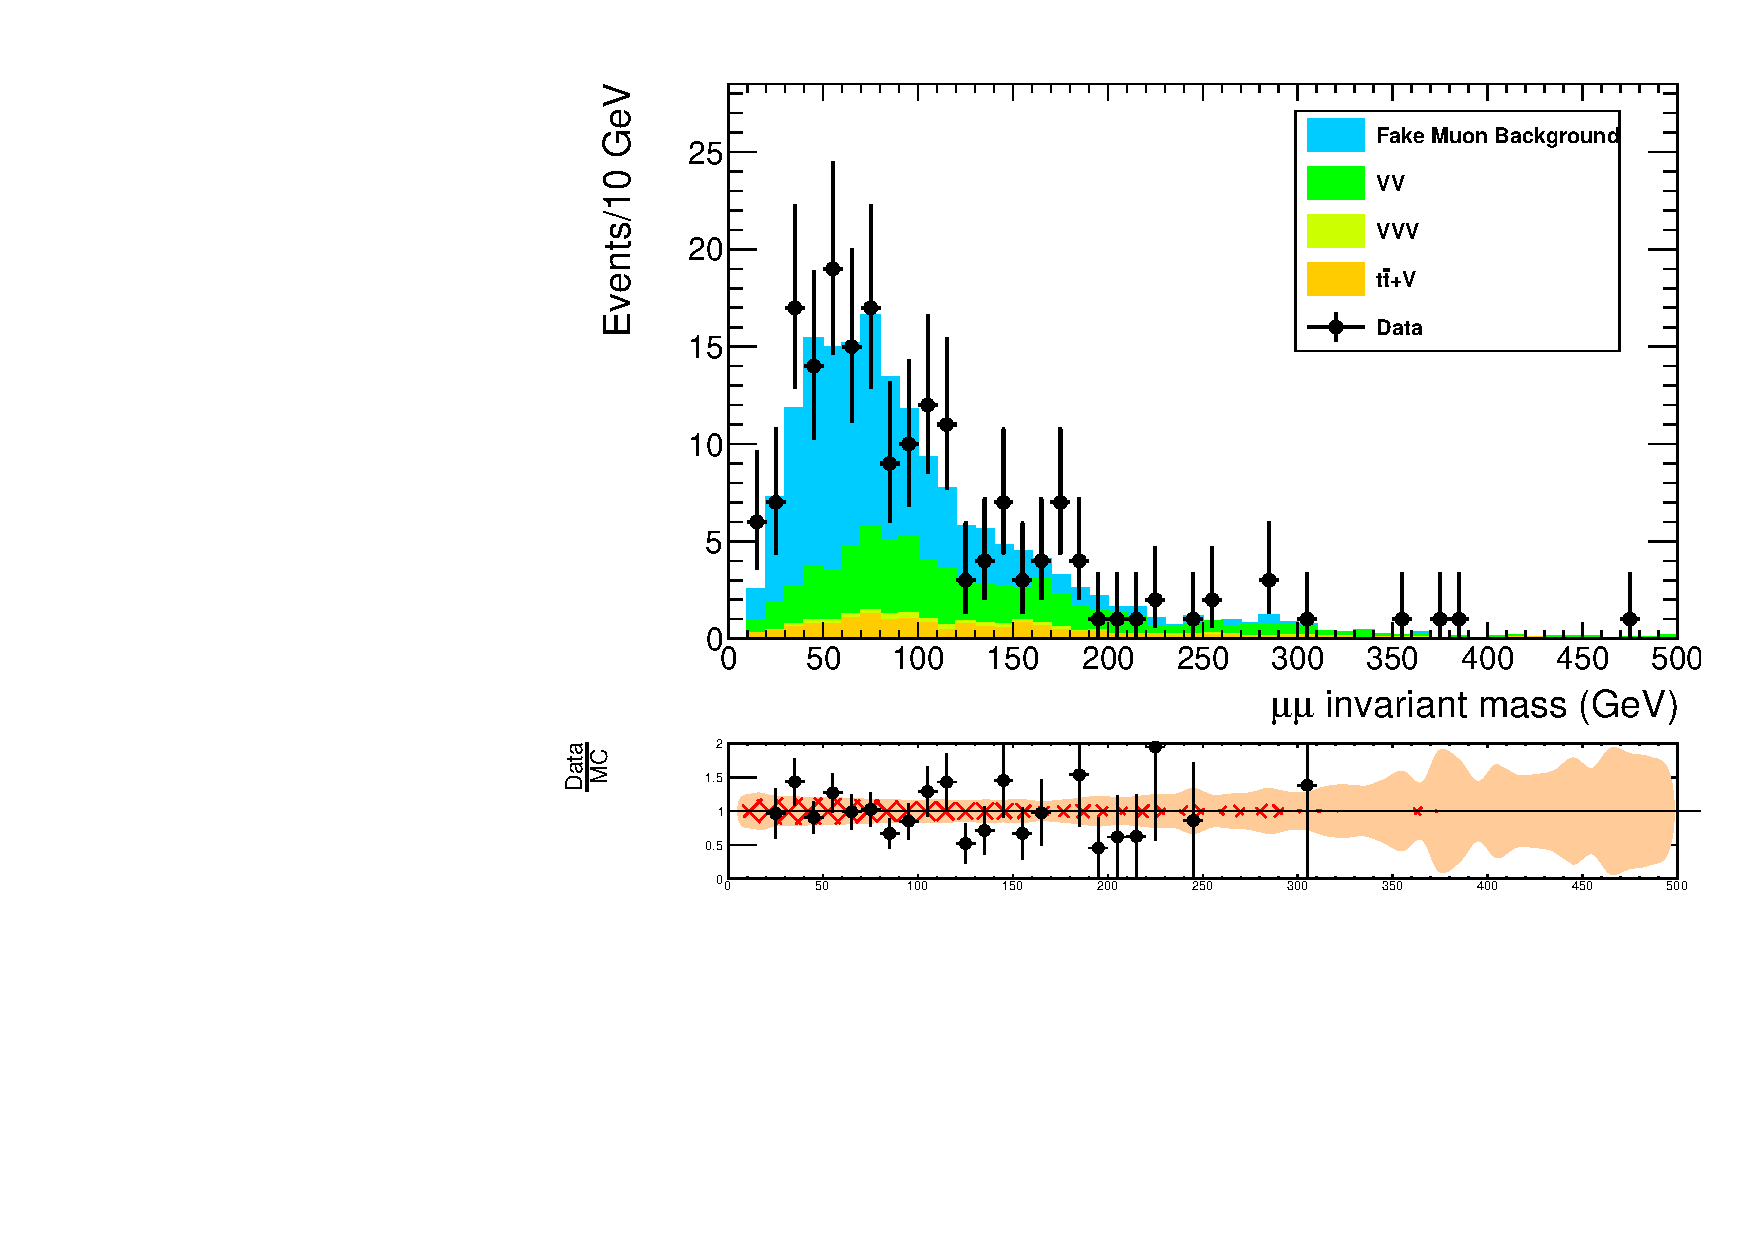
\includegraphics[scale=0.5]{figures/Ch_3_Selection/h_llmass_.pdf}
% 			\par\end{centering}
% 			\caption[The invariant mass of the two selected muons at preselection.]{\label{fig:mumuPreselection} The invariant mass of the two selected muons at preselection.  Light blue is the data-driven fake background, the others from MC simulation.  The ratio plot includes the systematic uncertainty on the fake background (red hatches) and the total uncertainty (systematic and statistical combined) on the background estimate (orange shaded region).}
% 		\end{figure}
% 		\begin{figure}
% 			\begin{centering}
% 				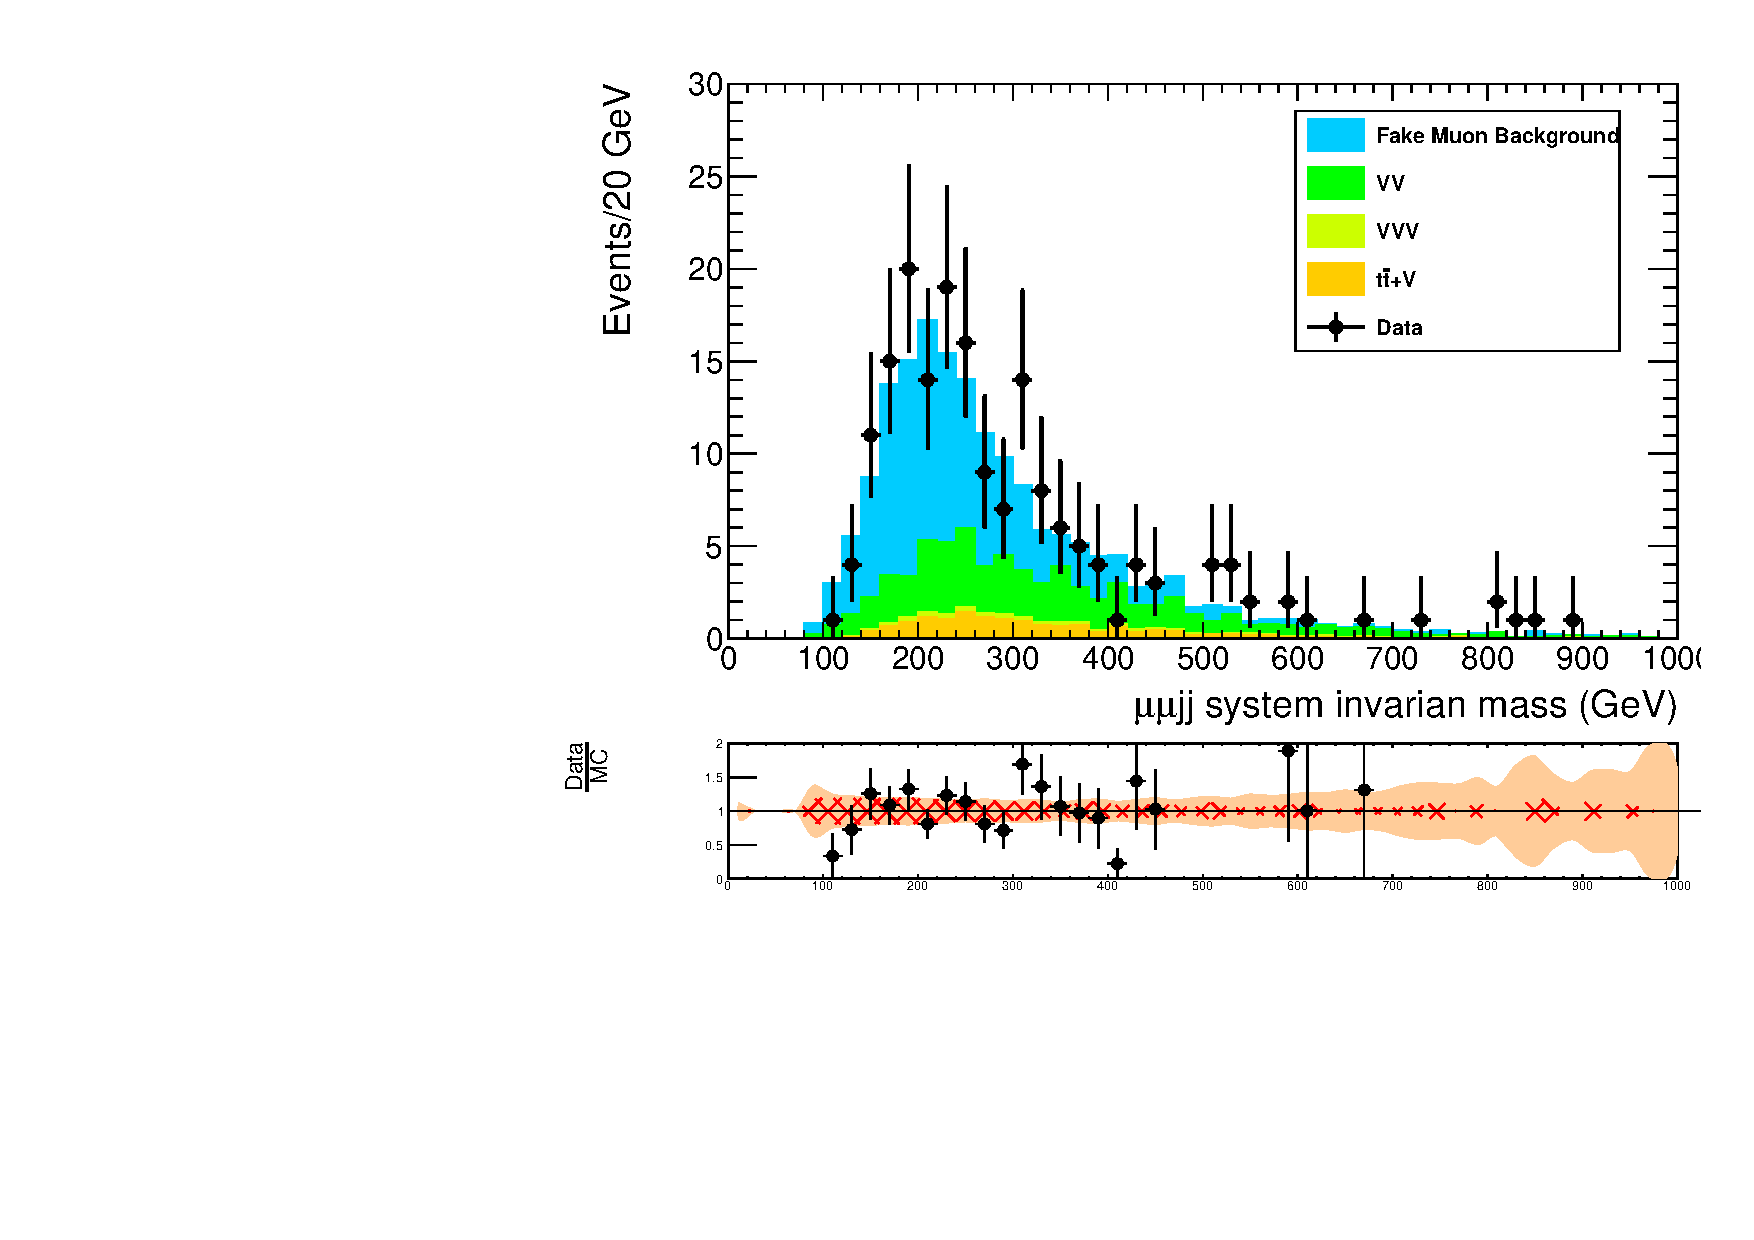
\includegraphics[scale=0.5]{figures/Ch_3_Selection/h_lljjmass_.pdf}
% 			\par\end{centering}
% 			\caption[The invariant mass of the two selected muons and two selected jets at preselection.]{\label{fig:mumujjPreselection} The invariant mass of the two selected muons and two selected jets at preselection.  Light blue is the data-driven fake background, the others from MC simulation.  The ratio plot includes the systematic uncertainty on the fake background (red hatches) and the total uncertainty (systematic and statistical combined) on the background estimate (orange shaded region).}
% 		\end{figure}
% 		%%%%%%%%%%%%%%%%%%%%%%%%%%%%%%%%%%%%%%%%%%%%%%%%%%%%%%%%%%%%%%%%%%%%%%%%%%%%%%%%%%

% 	\subsection{Full Selection}\label{section:fullselection}
% 		After pre-selection cuts are applied, the search is split into two mass regions.  The first region, corresponding to a heavy Majorana neutrino with a mass between 40 and 90 GeV/$c^2$, is referred to as the:
% 		\begin{description}
% 			\centering \item[Low Mass Region]
% 		\end{description}
% 		and the second, corresponding to a mass $\ge$ 90 GeV/$c^2$, dubbed the:

% 		\begin{description}
% 			\centering \item[High Mass Region]
% 		\end{description}

% 		The motivation for this is to separate regions based on whether the W-boson propagator is on-shell or not.

% 		In the low mass region, the $W$-propagator, (the first W boson in the Feynman diagram), is on-shell and the final state particles ($\mu^{\pm}\mu^{\pm}q\bar{q}'$) should have an invariant mass close to the mass of the $W$.  The following is a list of the selection criteria for the low mass region:

% 		\begin{itemize}
% 			\item[(a)] Low Mass Majorana Neutrino Selection (40 GeV/c$^2 < M_N < 90$ GeV/c$^2$)
% 			\begin{itemize}
% 				\item Any events with one or more b-tags (using the CSV Medium working point) are excluded (see Section \ref{section:btagJets}).
% 				\item Missing transverse energy (MET) must be less than 30 GeV.
% 				\item The invariant mass of the two muons and the two jets $m(\mu \mu j j) < $ 200 GeV/$c^2$, where the two jets chosen are those which result in $m(\mu^\pm \mu^\pm j j)$ closest to the $W$ mass.
% 				\item The invariant mass of two jets $m(jj)$ must be $<$ 120 GeV/$c^2$, where the two jets used are the same ones selected for the $m(\mu^\pm \mu^\pm j j)$ cut.
% 			\end{itemize}
% 		\end{itemize}

% 		In the high mass search region, ($m_N \ge 90$ GeV/$c^2$), the W-propagator is off-shell but the W-boson from the HMN decay is on-shell, meaning the $W \rightarrow q {\bar q}^\prime$ decay should result in a dijet invariant mass close to $m_W$. In this region the following  selection cuts are required:
% 		\begin{itemize}
% 			\item[(b)] High Mass Majorana Neutrino Selection ($M_N \ge 90$ GeV/$c^2$)
% 			\begin{itemize}
% 				\item Any events with one or more b-tags (using the CSV Medium working point) are excluded (see Section \ref{section:btagJets}).
% 				\item The dimuon invariant mass $m(\mu \mu)$ must be $> 15$ GeV/$c$ (in order to completely exclude the $\Upsilon$).
% 				\item The missing transverse energy (MET) must be $<$ 35 GeV.
% 				\item The dijet invariant mass must satisfy $50 < m(jj) < 110$ GeV/$c^2$,
% 				where the two jets with an invariant mass  closest to the $W$ mass are chosen.
% 			\end{itemize}
% 		\end{itemize}

% 		In order to understand the background, a \textit{control region} was defined using the same event signature, while requiring an independent variable that ensures the signal is excluded.  For example, there should be no b-quarks generated in this signal, and by requiring a b-tagged jet in the control region, any events studied should consist only of background processes to the signal of interest.

% 		The following criteria define the control regions used:

% 		\begin{itemize}
% 			\item[(a)] Low Mass Control Region ($40$ GeV/$c^2 < M_N < 90$ GeV$/c^2$)
% 			\begin{itemize}
% 				  \item The selection is the same as the low mass signal selection, except:
% 				  \item (missing transverse energy (MET) must be $>$ 50 GeV)  OR (one or more b-tags must pass the CSV Medium working point, see Section \ref{section:btagJets})
% 			\end{itemize}

% 			\item[(b)] High Mass Control Region ($M_N \ge 90$ GeV/$c^2$)

% 			\begin{itemize}
% 				\item The selection is the same as the high mass signal selection, except:
% 				\item (The missing transverse energy (MET) must be $>$ 50 GeV)  OR (one or more b-tags must pass the CSV Medium working point, see Section \ref{section:btagJets})
% 			\end{itemize}
% 		\end{itemize}


% 	\subsection{Final Selection Optimization}\label{punziFoM}
% 		In the interest of completeness, the final selection optimization procedure is briefly described here, though the results are described in Section \ref{finalSelection}.

% 		A \textit{figure of merit} was used to optimize the final signal selection criteria as a function of HMN mass.  The figure of merit quantifies the goodness of the selection by comparing the signal with background while also incorporating the statistical significance of the expected signal.  The selection was optimized with the following three variables:

% 		\begin{itemize}
% 			  \item The transverse momentum of the leading muon, $p_{T, \mu 1}$.
% 			  \item The transverse momentum of the trailing muon, $p_{T, \mu 2}$.
% 			  \item The invariant mass of the two muons and two selected jets $m(\mu \mu j j)$.
% 		\end{itemize}
% 		with the Punzi (see \cite{punzi}) figure of merit:
% 		\begin{equation}
% 			\frac{\epsilon_S}{a/2 + \sqrt{N_t + (\delta N_f)^2}}
% 		\end{equation}
% 		Here, $\epsilon_S$ is the signal efficiency, $a$ is the number of standard deviations desired from the result (in this case $a = 2$ as is standard), and $\delta$ is the fractional systematic uncertainty on the fake background estimate (see Section \ref{sec:fake}). The second term in the denominator is the standard uncertainty on the background estimate plus -- in this specific case -- a fixed contribution of 28\% due to fake events, ($N_f$).  The results of this process are discussed in Section \ref{finalSelection}.


% \section{Selection Efficiency}\label{Section:selectionEfficiency}
% This section summarizes the efficiencies of the various selection criteria.  Each selection criteria's efficiency depends on specific traits intrinsic to the selection mechanism.  In other words, this analysis requires the selection of two muons, but what exactly is a muon according to CMS?  After all, CMS simply responds to a muon or other any other particle traversing its volume with a bundle of electrical pulses.  How is it that one bundle of electrical pulses can be determined to be an electron, while another bundle can be called a muon?  Increasing selection variables lead to increased confidence that the choice of particle being represented by the bundle of pulses is correct, but it also decreases the muon selection efficiency, hurting the overall statistics.  Not all muons create the same bundle of electrical pulses, and not all analyses require the same strictness.  The qualities used in this analysis to select the final particles, along with their efficiencies, are described below.

% 	\subsection{Trigger Efficiency}\label{triggerEfficiency}
% 		The muon trigger selection efficiencies along with their associated systematic uncertainties are taken directly from the muon POG, as detailed in Reference \cite{piet_talk}.  The muon trigger efficiency is p$_\text{T}$ and $\eta$ dependent, and is above 90\% for both the low mass and high mass search regions.

% 	\subsection{Offline Selection Efficiency}
% 		One of the most important studies in this analysis was the estimate of the selection efficiencies for the event signature as a function of HMN mass.  The goal is to understand the efficiencies of selecting two jets and two muons, and with all the described selection criteria.

% 		First, described in Table \ref{table:muoncuts}, is the selection efficiency of the same-sign muons.  Of note is the dip in selection efficiency when the HMN mass is between 70 and 90 GeV/$c^2$.  This is due to the nature of the production process;  if the HMN is near the $W$ mass, the produced muons will be too \textit{soft}; i.e., their p$_\text{T}$ will be too low to pass our selection criteria, leading to a drop in efficiency.

% 		To calculate these efficiencies, a suite of software was written to create nTuples of the signal Monte Carlo samples filled with quantities the analysis would use for selection criteria.  A separate analysis package was written to analyze the data and calculate the efficiencies for the final state particles with very fine resolution, allowing the understanding of which cuts were causing the largest drops in efficiencies.  This process resulted in high optimization of the preselection criteria.

% 		The overall selection efficiency of the signal signature is listed in Table \ref{table:allcuts}.  Also in Table \ref{table:allcuts} are the estimated numbers of events expected in our dataset with an integrated luminosity of 19.7 fb$^{-1}$.

% 		\begin{table}
% 			\centering
% 			\caption{Muon selection and individual cut efficiencies for events in Signal MC passing the selection cuts listed in Sections~\ref{subsec:muonSelection} -- \ref{section:fullselection}.}
% 			\label{table:muoncuts}
% 			\begin{center}
% 				\begin{tabular*}{\textwidth}{@{\extracolsep{\fill}}c c cccc}
% 					\hline
% 					Generated     & Total  & \multicolumn{4}{c}{\% Events Accepted}\\
% 					HMN Mass & Events & Track Quality   & $\eta$ and p$_\text{T}$ & Isolation & All\\
% 					\hline
% 					40 GeV/\(c^2\)		& 99390 & 46.0 $\pm$ 0.2 & 15.8 $\pm$ 0.1 & 21.5 $\pm$ 0.1 & 7.12 $\pm$ 0.08\\
% 					60 GeV/\(c^2\)		& 99494 & 49.3 $\pm$ 0.2 & 11.0 $\pm$ 0.1 & 21.2 $\pm$ 0.1 & 4.72 $\pm$ 0.07\\
% 					70 GeV/\(c^2\)		& 49994 & 44.9 $\pm$ 0.2 & 3.3 $\pm$ 0.1 & 17.0 $\pm$ 0.2 & 1.37 $\pm$ 0.05\\
% 					80 GeV/\(c^2\)		& 98492 & 37.1 $\pm$ 0.2 & 12.1 $\pm$ 0.1 & 15.7 $\pm$ 0.1 & 5.50 $\pm$ 0.07\\
% 					90 GeV/\(c^2\)		& 49996 & 50.2 $\pm$ 0.2 & 10.0 $\pm$ 0.1 & 19.0 $\pm$ 0.2 & 3.62 $\pm$ 0.08\\
% 					100 GeV/\(c^2\)	& 49996 & 59.7 $\pm$ 0.2 & 29.3 $\pm$ 0.2 & 27.5 $\pm$ 0.2 & 12.3 $\pm$ 0.2\\
% 					125 GeV/\(c^2\)	& 49995 & 67.4 $\pm$ 0.2 & 56.6 $\pm$ 0.2 & 40.5 $\pm$ 0.2 & 30.2 $\pm$ 0.2\\
% 					150 GeV/\(c^2\)	& 49995 & 71.5 $\pm$ 0.2 & 65.2 $\pm$ 0.2 & 47.5 $\pm$ 0.2 & 37.7 $\pm$ 0.2\\
% 					175 GeV/\(c^2\)	& 49995 & 74.9 $\pm$ 0.2 & 69.9 $\pm$ 0.2 & 52.3 $\pm$ 0.2 & 42.2 $\pm$ 0.2\\
% 					200 GeV/\(c^2\)	& 49992 & 77.3 $\pm$ 0.2 & 73.7 $\pm$ 0.2 & 55.7 $\pm$ 0.2 & 45.7 $\pm$ 0.2\\
% 					250 GeV/\(c^2\)	& 49997 & 81.0 $\pm$ 0.2 & 78.0 $\pm$ 0.2 & 58.7 $\pm$ 0.2 & 48.7 $\pm$ 0.2\\
% 					300 GeV/\(c^2\)	& 49996 & 83.4 $\pm$ 0.2 & 81.0 $\pm$ 0.2 & 60.7 $\pm$ 0.2 & 50.4 $\pm$ 0.2\\
% 					350 GeV/\(c^2\)	& 49995 & 84.9 $\pm$ 0.2 & 82.5 $\pm$ 0.2 & 60.7 $\pm$ 0.2 & 50.1 $\pm$ 0.2\\
% 					400 GeV/\(c^2\)	& 49996 & 85.8 $\pm$ 0.2 & 83.8 $\pm$ 0.2 & 60.7 $\pm$ 0.2 & 50.3 $\pm$ 0.2\\
% 					500 GeV/\(c^2\)	& 49995 & 86.4 $\pm$ 0.2 & 84.2 $\pm$ 0.2 & 59.1 $\pm$ 0.2 & 48.6 $\pm$ 0.2\\
% 					%600 GeV/\(c^2\)	& 49994 & 85.7 $\pm$ 0.16 & 83.3 $\pm$ 0.17 & 57.0 $\pm$ 0.22 & 46.4 $\pm$ 0.22  \\
% 					%700 GeV/\(c^2\)	& 49998 & 84.4 $\pm$ 0.16 & 81.2 $\pm$ 0.17 & 54.8 $\pm$ 0.22 & 44.3 $\pm$ 0.22  \\
% 					\hline
% 				\end{tabular*}
% 				\begin{tablenotes}
% 					\item	Note: Errors are statistical only.
% 				\end{tablenotes}
% 			\end{center}
% 		\end{table}


% 		\begin{table}
% 			\centering
% 			\caption{Event selection efficiencies for the events in Signal MC passing the selection cuts listed in Sections~\ref{subsec:muonSelection} -- \ref{section:fullselection}.}
% 			\label{table:allcuts}
% 			\begin{center}
% 				\begin{tabular*}{\textwidth}{@{\extracolsep{\fill}}c c ccc l}
% 					\hline
% 					Generated    		 & Total   	& \multicolumn{3}{c}{\% Events Accepted}                          			& \# of Events\\
% 					HMN Mass 		& Events	& All Muon            	& Jets                	 	& All Cuts            		& for $19.$7 fb$^{-1}$\\
% 					\hline
% 					40 GeV/\(c^2\)		& 99390 	& 7.12 $\pm$ 0.08 	& 19.3 $\pm$ 0.1 	& 0.741 $\pm$ 0.027 	& 2216670 $\pm$ 8290  \\
% 					60 GeV/\(c^2\)		& 99494 	& 4.72 $\pm$ 0.07 	& 23.3 $\pm$ 0.1 	& 0.722 $\pm$ 0.027 	& 86654 $\pm$ 3281  \\
% 					70 GeV/\(c^2\)		& 49994	& 1.37 $\pm$ 0.05 	& 30.1 $\pm$ 0.2 	& 0.278 $\pm$ 0.024 	& 11646 $\pm$ 1004  \\
% 					80 GeV/\(c^2\)		& 98942 	& 5.50 $\pm$ 0.07   	& 42.5 $\pm$ 0.2 	& 1.233 $\pm$ 0.035 	& 4644 $\pm$ 135  \\
% 					90 GeV/\(c^2\)		& 49996 	& 3.62 $\pm$ 0.08 	& 55.8 $\pm$ 0.2 	& 0.788 $\pm$ 0.04 		& 1106 $\pm$ 56  \\
% 					100 GeV/\(c^2\)	& 49996 	& 12.3 $\pm$ 0.2 	& 58.5 $\pm$ 0.2 	& 4.970 $\pm$ 0.097 	& 3500 $\pm$ 69  \\
% 					125 GeV/\(c^2\)	& 49995 	& 30.2 $\pm$ 0.2 	& 65.2 $\pm$ 0.2 	& 13.15 $\pm$ 0.151 	& 2798 $\pm$ 33  \\
% 					150 GeV/\(c^2\)	& 49995 	& 37.7 $\pm$ 0.2 	& 70.1 $\pm$ 0.2 	& 16.72 $\pm$ 0.167 	& 1518 $\pm$ 15  \\
% 					175 GeV/\(c^2\)	& 49995 	& 42.2 $\pm$ 0.2 	& 73.6 $\pm$ 0.2 	& 19.14 $\pm$ 0.176 	& 880 $\pm$ 8  \\
% 					200 GeV/\(c^2\)	& 49992 	& 45.7 $\pm$ 0.2 	& 76.6 $\pm$ 0.2 	& 20.88 $\pm$ 0.182 	& 542 $\pm$ 5  \\
% 					250 GeV/\(c^2\)	& 49997 	& 48.7 $\pm$ 0.2 	& 80.4 $\pm$ 0.2 	& 22.84 $\pm$ 0.188 	& 230 $\pm$ 3  \\
% 					300 GeV/\(c^2\)	& 49996 	& 50.4 $\pm$ 0.2 	& 82.5 $\pm$ 0.2 	& 23.39 $\pm$ 0.189 	& 107.3 $\pm$ 0.9  \\
% 					350 GeV/\(c^2\)	& 49995 	& 50.1 $\pm$ 0.2 	& 83.5 $\pm$ 0.2 	& 22.71 $\pm$ 0.187 	& 52.5 $\pm$ 0.5  \\
% 					400 GeV/\(c^2\)	& 49996 	& 50.3 $\pm$ 0.2 	& 83.6 $\pm$ 0.2 	& 22.31 $\pm$ 0.186 	& 27.9 $\pm$ 0.3  \\
% 					500 GeV/\(c^2\)	& 49995 	& 48.6 $\pm$ 0.2 	& 82.4 $\pm$ 0.2 	& 19.70 $\pm$ 0.178 	& 8.4 $\pm$ 0.1  \\
% 					%600 GeV/\(c^2\)	& 49994 	& 46.4 $\pm$ 0.22 	& 80.0 $\pm$ 0.18 	& 17.17 $\pm$ 0.169 	& 2.90 $\pm$ 0.03  \\
% 					%700 GeV/\(c^2\)	& 49998 	& 44.3 $\pm$ 0.22 	& 77.5 $\pm$ 0.19 	& 15.52 $\pm$ 0.162 	& 1.18 $\pm$ 0.01  \\
% 					\hline
% 				\end{tabular*}
% 				\begin{tablenotes}
% 					\item	Note: Errors are statistical only.
% 				\end{tablenotes}
% 			\end{center}
% 		\end{table}


% 	\subsection{Tag and Probe Study}\label{tnp}
% 		One of the most intensive aspects of this analysis was a so-called \textit{tag and probe} study.  The tag and probe method for this analysis is used to compare muon selection efficiencies in data and MC in order to calculate the so-called \textit{Data/MC scale factor}.\footnote{For an in-depth description of the tag and probe method, see \cite{HiggsToWWToLL, SUSY_2010, SUSY_2011, LepEff}.}

% 		The tag and probe method is a data-driven technique used to calculate efficiencies.  In this analysis, the efficiency of the muon reconstruction is an important quantity, and with our signal sample created using a Monte Carlo generator, the MC performance must be compared with data to ensure the accuracy of the simulation.  This directly effects the estimation of the signal.  Normally, the muon POG takes care of these calculations and the user can simply incorporate the efficiencies and scale factors directly into their analysis.  However, during the early phases of the analysis, it was discovered that a lower \textit{Relative Isolation} (RelIso) than the standard POG value improved the figure of merit.  Therefore, the tag and probe method was deployed to understand the effect of tightening this requirement on muon efficiency in both data and MC.

% 		The method requires a known mass resonance with preferably a low background.  The subject of the analysis is the muon, making a perfect candidate of the $Z \rightarrow \mu^\pm \mu^\mp$ Drell-Yan process.  The tag and the probe are a \textit{tight} and a \textit{loose} muon, respectively.

% 		The method begins by choosing a muon with very tight selection requirements as the tag, and a probe muon with only basic qualities like minimum p$_\text{T}$ and $\eta$ requirements.  The efficiency is defined as:
% 		%
% 		\begin{equation}
% 			\epsilon = \frac{TP}{(TP + TF)}
% 		\end{equation}
% 		where TP represents the two muons:  The first letter in a pair representing the tag muon, and the second letter representing the state defining whether or not the probe muon passed or failed.  TP = Tag and passing probe, TF = Tag and failing probe.

% 		Only events containing exactly 2 muons were considered and only events with muons having opposite charge were considered\footnote{This was required in order to reduce selecting muons from other processes.}.  After an event is found containing two ``loose'' muons, the algorithm checks to see if one of them matches the muon which triggered the event (with $\Delta$R matching and a truth boolean in the ntuple (labeled MuonHLTSingleIsoMuonMatched)), and then asks if the triggered muon passes the tight tag requirements.  If it does, its properties and ID are stored and its index is labeled as the tag muon.

% 		Next it checks to see if the second muon, which has already passed the `probe' criteria, also passes the `tight' criteria.  If it passes, the tag/probe pair's combined mass is stored in a histogram labeled `Pass'.  If it fails, the tag/probe pair's mass is stored into a histogram labeled `Fail'.

% 		After populating the pass and fail histograms by running over all the events, the efficiency can be calculated by determining the number of events which pass and the number of events which fail.  In order to differentiate true Z decay muons from background muons, the pass/fail yields are determined by using fits that are applied to the histograms.  The histograms are fit using the RooFit package with a sum of two \textit{voigtian} functions representing the signal, and an exponential function representing the background\footnote{This is to accurately account for both the Z decay shape and the distribution widening from detector resolution effects.}.  The mean of the fits are bound to 90-92 GeV/$c^2$.

% 		Figures \ref{fig:DataPassID} and \ref{fig:MCPassID} show examples of the Z mass peak fits used to estimate the signal yield.  In these figures, the left plot is used to determine the TP quantity, and the right plot is used to determine the TF quantity.

% 		In order to understand the efficiency as a function of muon p$_\text{T}$, this process was repeated for 12 separate p$_\text{T}$ regions, and 4 distinct $\eta$ regions.  The final efficiencies for both data and MC, including their scale factors (data/MC), as a function of p$_\text{T}$ and $\eta$, can be studied in Figures \ref{fig:DataMC_eta0} and \ref{fig:DataMC_eta1}.  This same information is displayed in tabular form in Tables \ref{table:TPmuon1} and \ref{table:TPmuon2}.

% 		These results (with scale factors close to 1) show that the muons in our selected range are well modeled by Monte Carlo simulations.  The scale factors are then used to rescale the MC datasets\footnote{An overall systematic of 2\% was used for the muon selection, as described in Section \ref{systematics}.}.


% 		%%%%%%%%%%%%%%%%%%%%%%%%%%%%%%%%%%% Tag and Probe Pass & Fail %%%%%%%%%%%%%%%%%%%%%%%%%%%%%%%%%%%%%%%%
% 		\begin{figure}
% 			\begin{centering}
% 				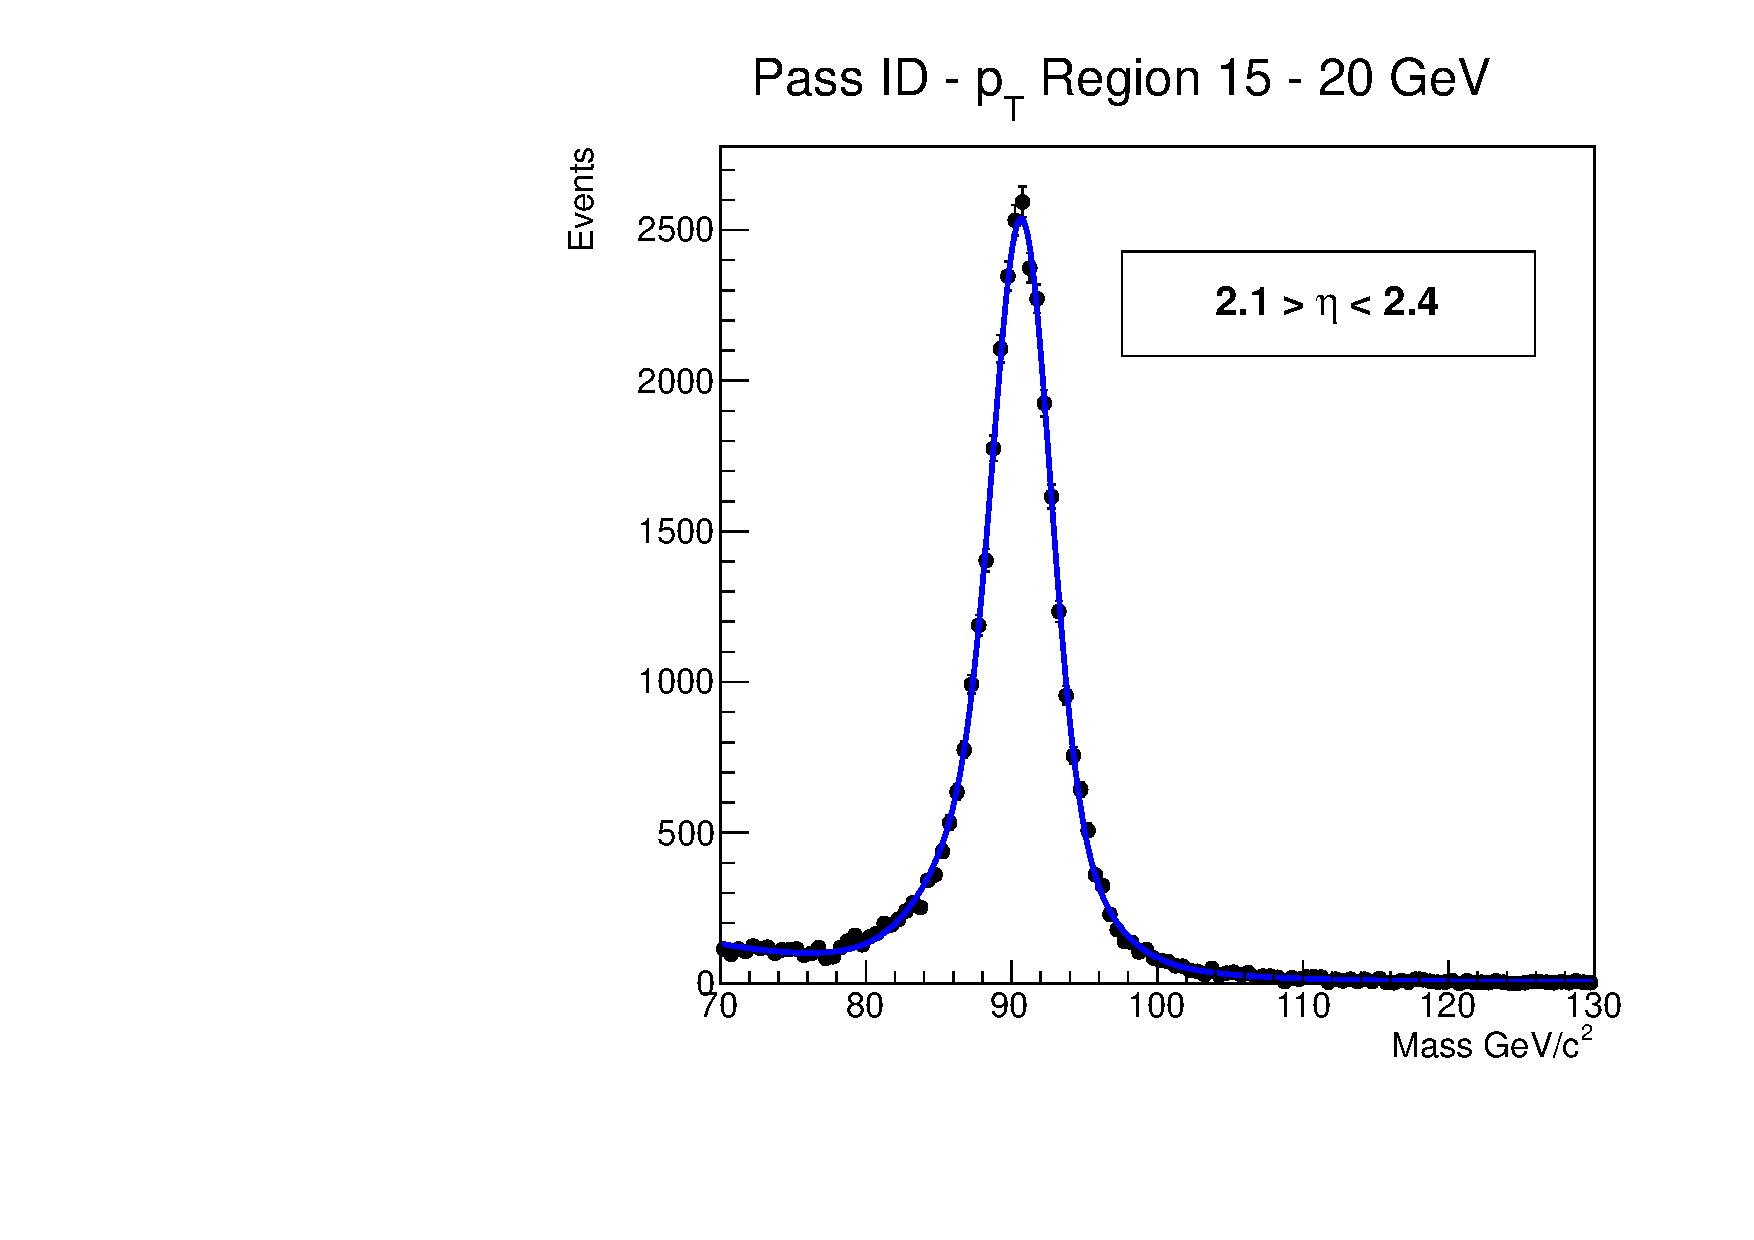
\includegraphics[scale=0.37]{figures/Ch_3_Selection/TagAndProbe/DataPass_ID_03.pdf}
% 				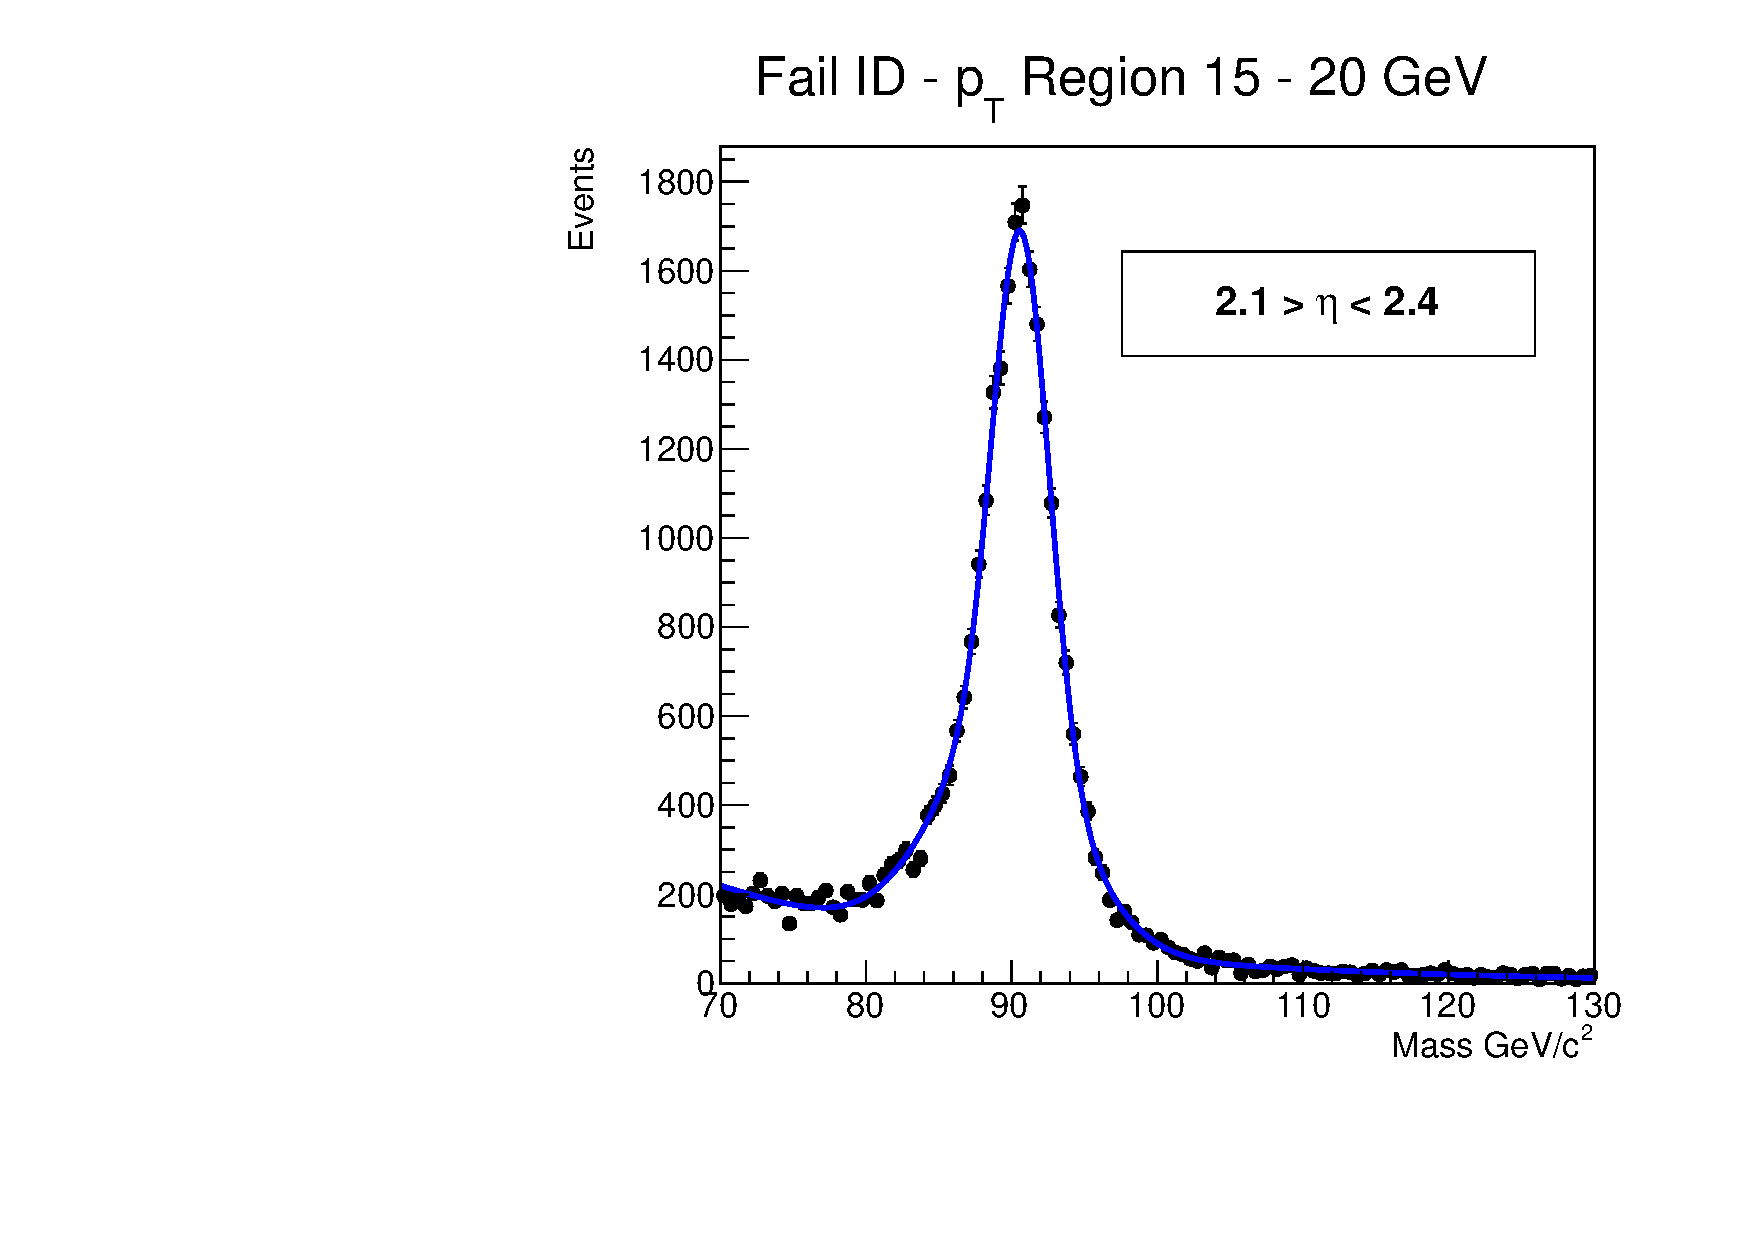
\includegraphics[scale=0.37]{figures/Ch_3_Selection/TagAndProbe/DataFail_ID_03.pdf}
% 			\par\end{centering}
% 			\caption[Example Z Boson mass peak from $Z\rightarrow \mu\mu$ in collision data.]{\label{fig:DataPassID}Example Z Boson mass peak from $Z\rightarrow \mu\mu$ in collision data.  Pass (left) and fail (right) histograms used in the tag and probe study.  See Section \ref{tnp} for a detailed description.}
% 			\vspace{25.0mm}
% 			\begin{centering}
% 				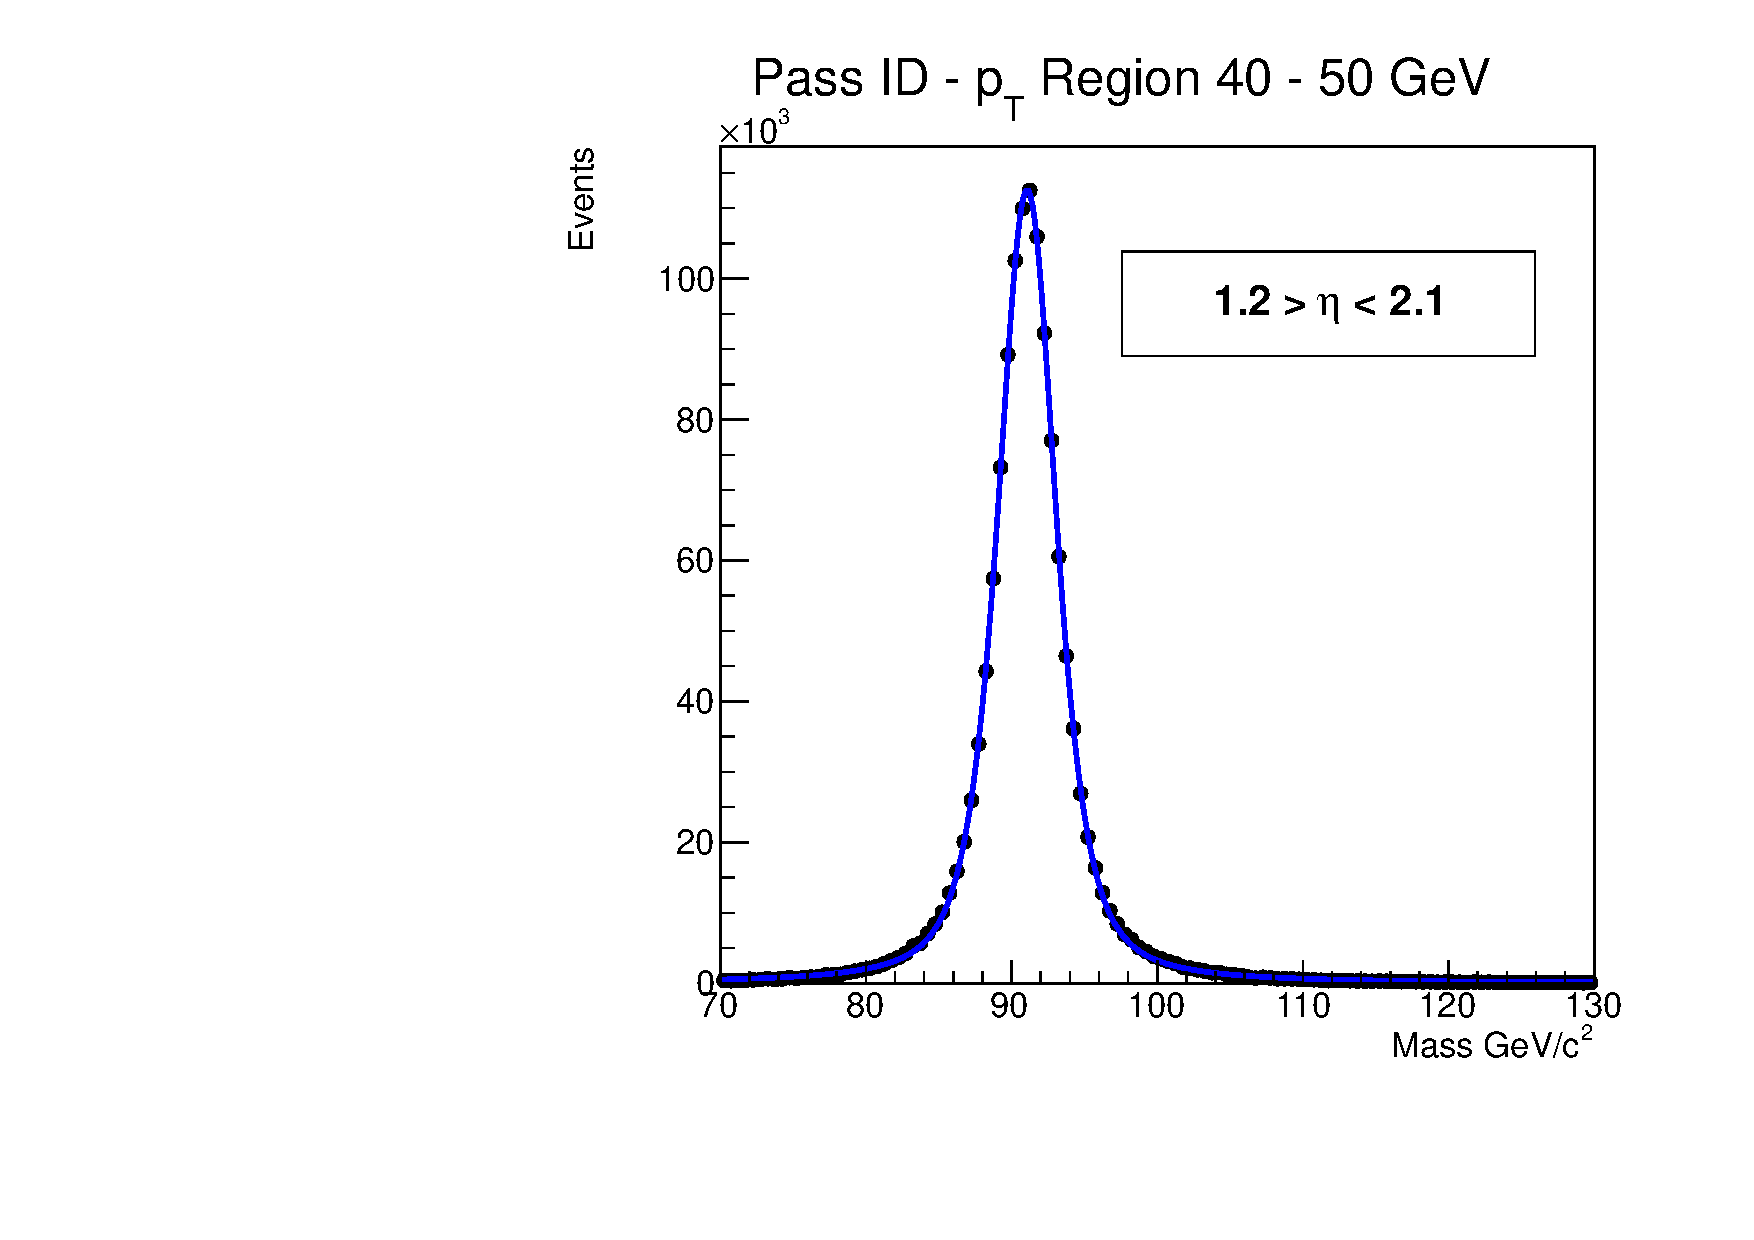
\includegraphics[scale=0.37]{figures/Ch_3_Selection/TagAndProbe/MC_Pass_ID_32.pdf}
% 				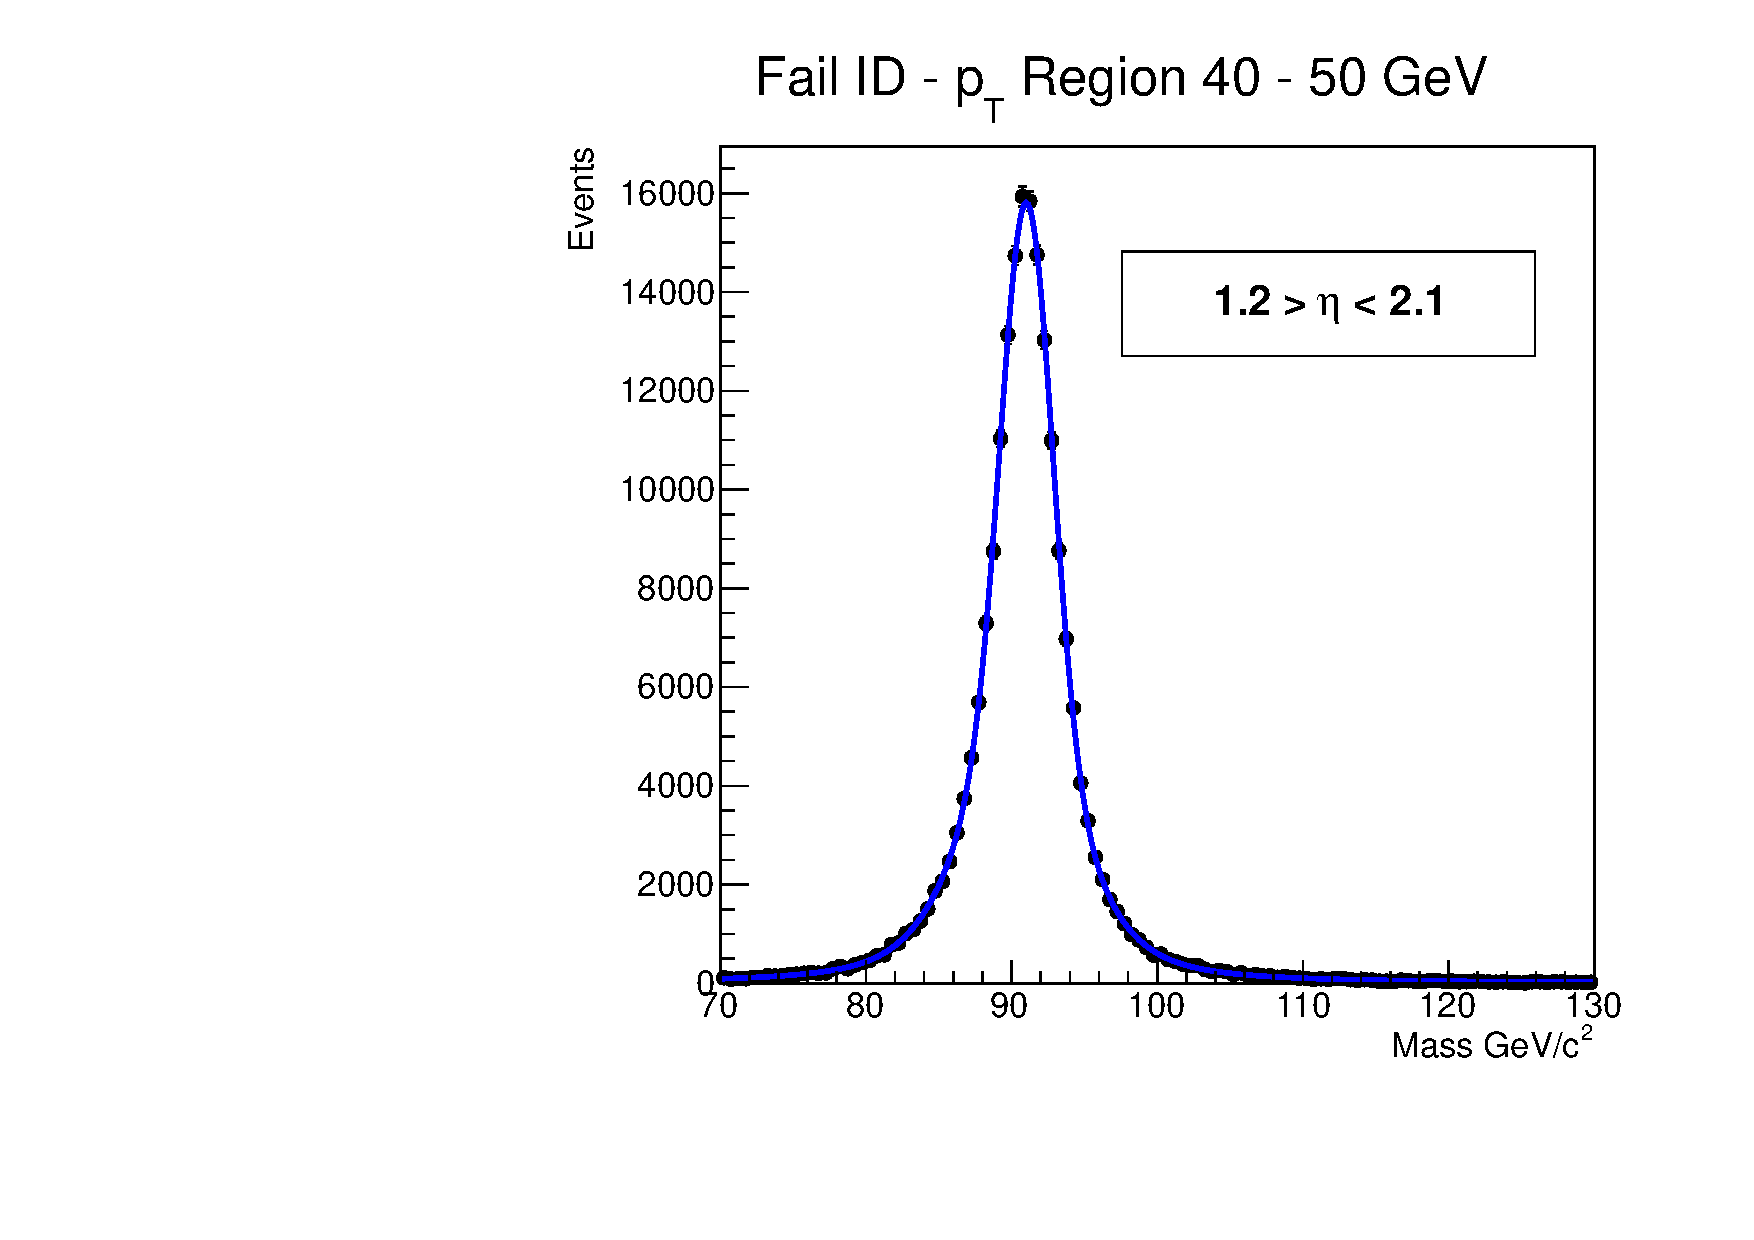
\includegraphics[scale=0.37]{figures/Ch_3_Selection/TagAndProbe/MC_Fail_ID_32.pdf}
% 			\par\end{centering}
% 			\caption[Example Z Boson mass peak from $Z\rightarrow \mu\mu$ in Monte Carlo data.]{\label{fig:MCPassID}Example Z Boson mass peak from $Z\rightarrow \mu\mu$ in Monte Carlo data.  Pass (left) and fail (right) histograms used in the tag and probe study.  See Section \ref{tnp} for a detailed description.}
% 		\end{figure}
% 		%%%%%%%%%%%%%%%%%%%%%%%%%%%%%%%%%%%%%%%%%%%%%%%%%%%%%%%%%%%%%%%%%%%%%%%%%%%%%%%%%%%%%%%%%


% 		%%%%%%%%%%%%%%%%%%%%%%%%%%%%%%%%%%% Data MC Scale Factor %%%%%%%%%%%%%%%%%%%%%%%%%%%%%%%%%%%%%%%%%%
% 		\begin{figure}
% 			\begin{centering}
% 				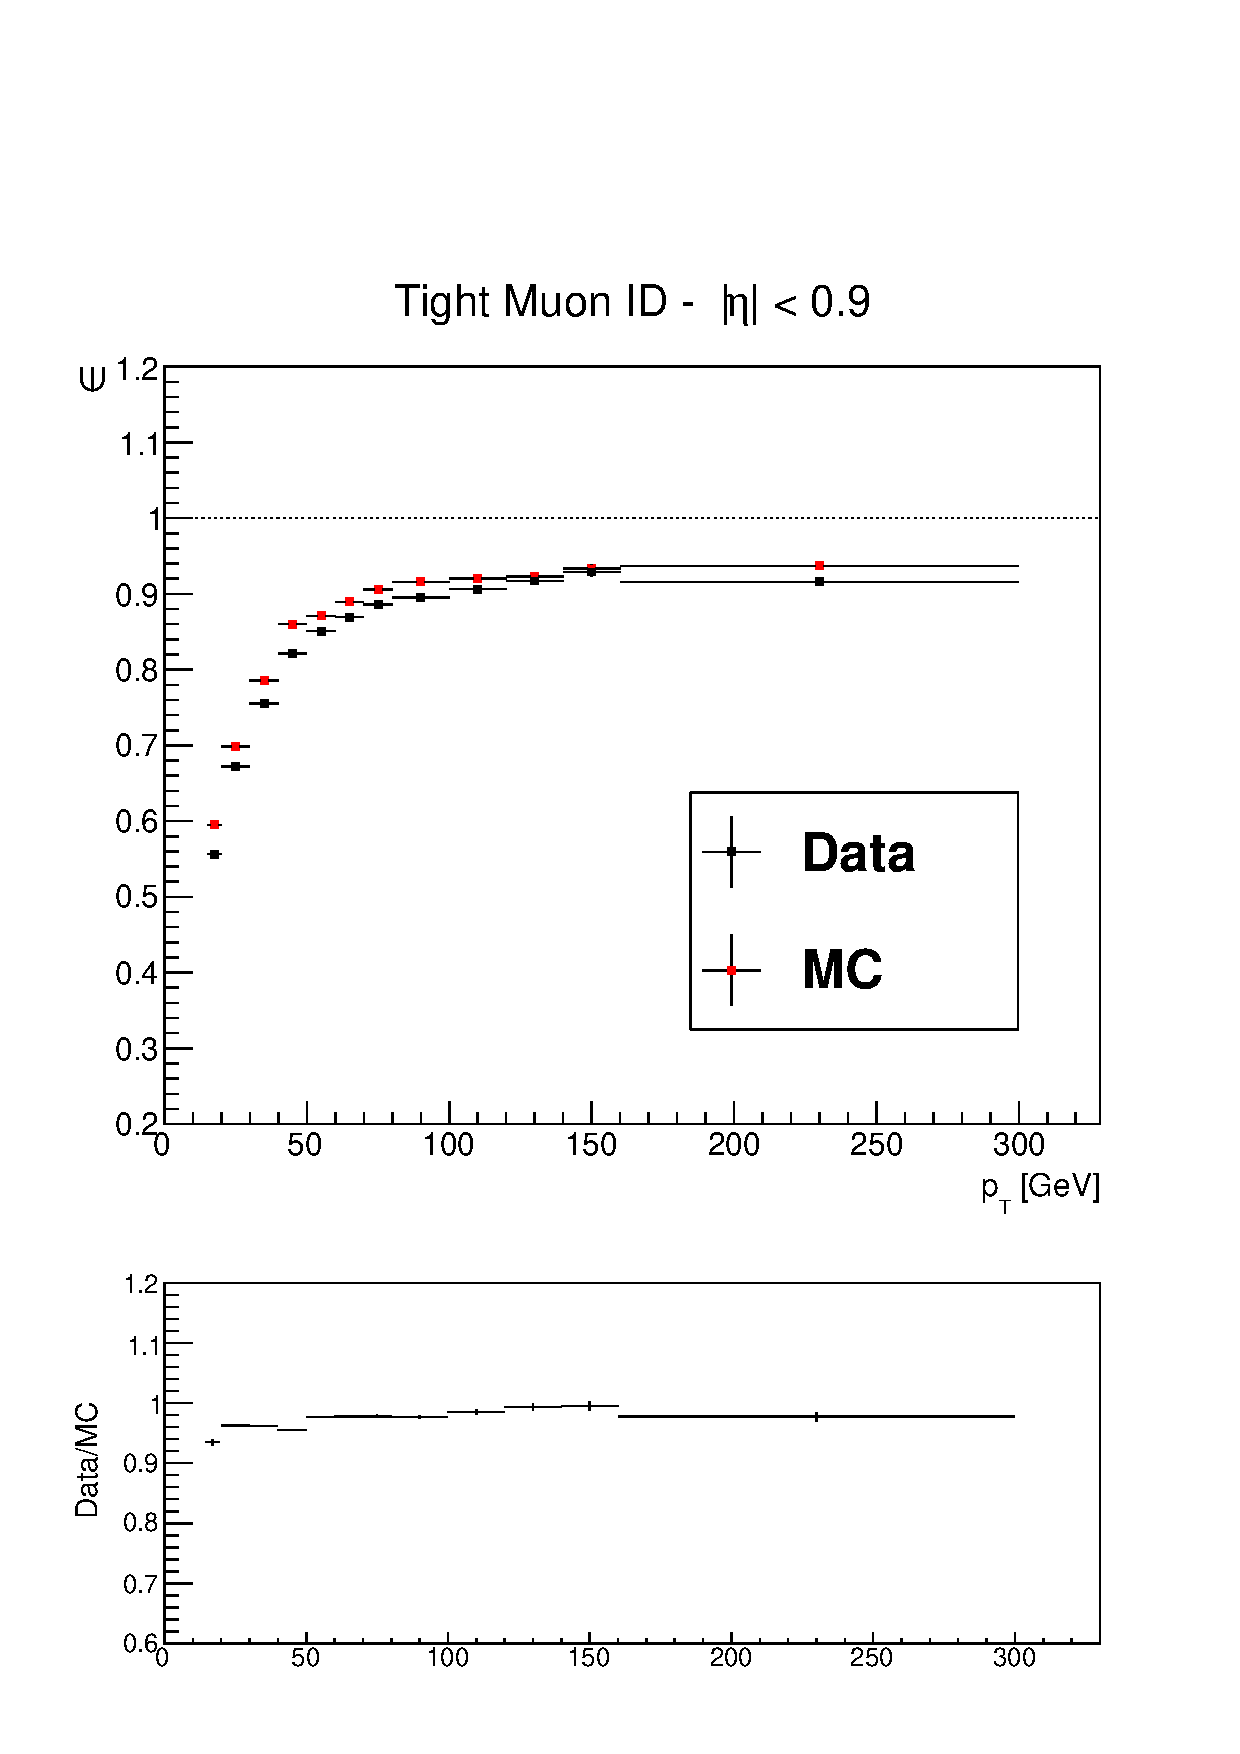
\includegraphics[scale=0.37]{figures/Ch_3_Selection/TagAndProbe/0PassId.pdf}
% 				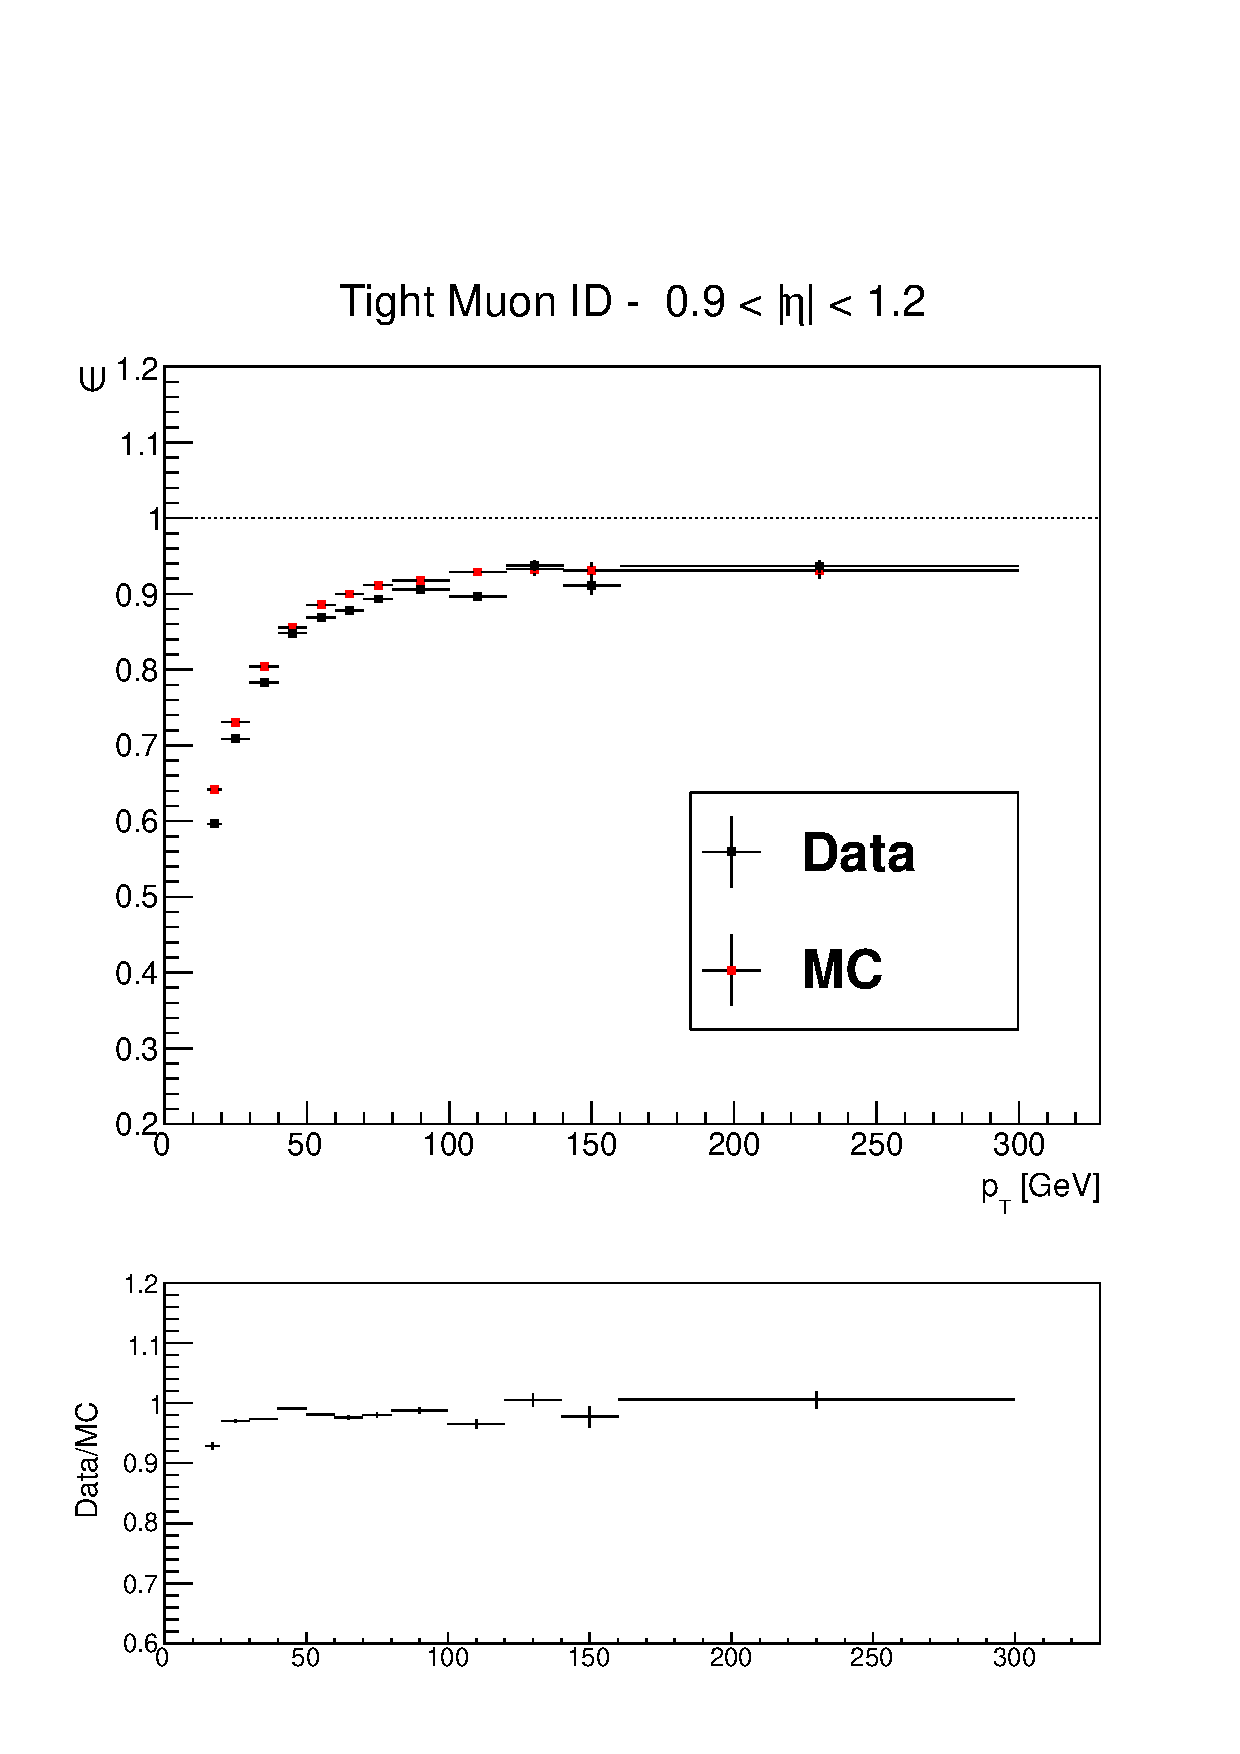
\includegraphics[scale=0.37]{figures/Ch_3_Selection/TagAndProbe/1PassId.pdf}
% 			\par\end{centering}
% 			\caption[Muon Efficiencies using the Tag and Probe method for $\eta$ 0 -- 1.2]{\label{fig:DataMC_eta0}Muon Efficiencies using the Tag and Probe method for $|\eta|$ 0 -- 1.2.}
% 			\vspace{25.0mm}
% 			\begin{centering}
% 				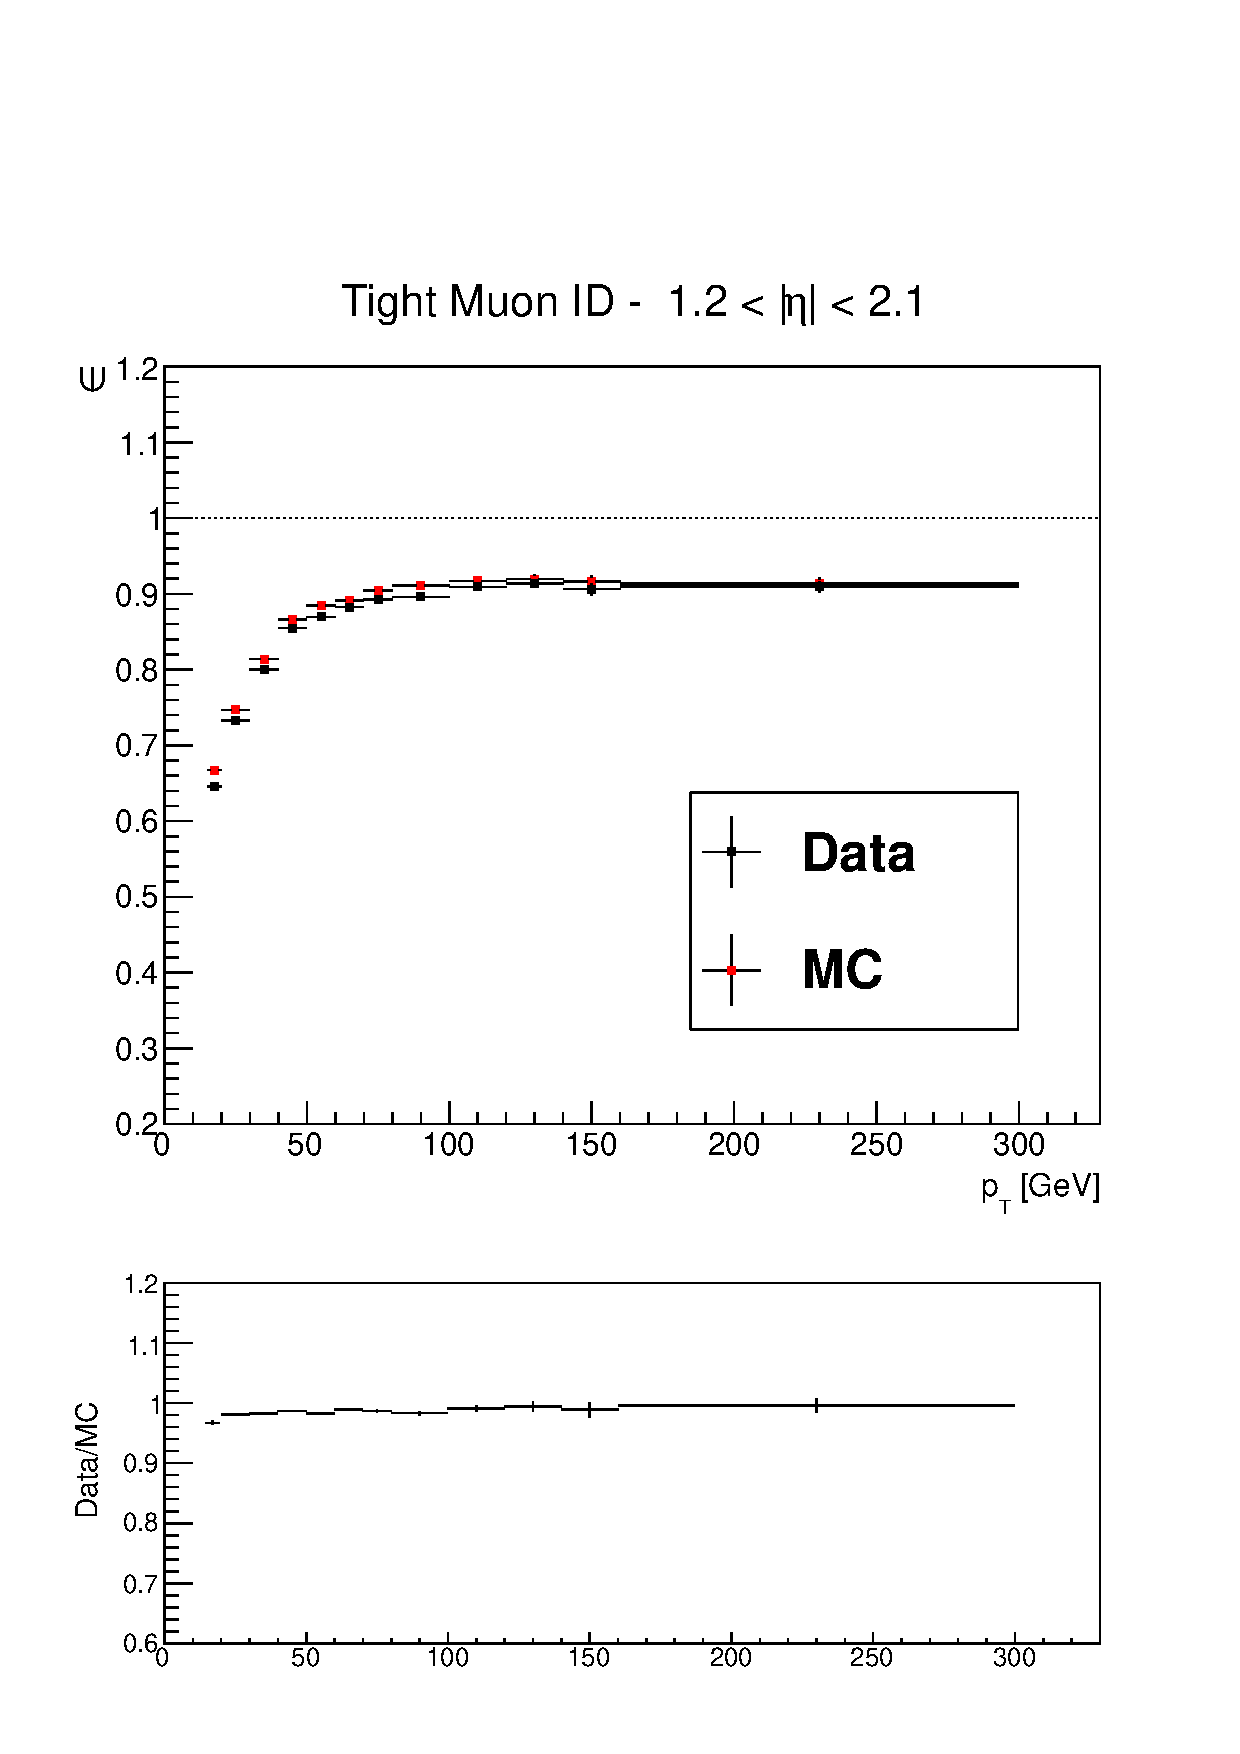
\includegraphics[scale=0.37]{figures/Ch_3_Selection/TagAndProbe/2PassId.pdf}
% 				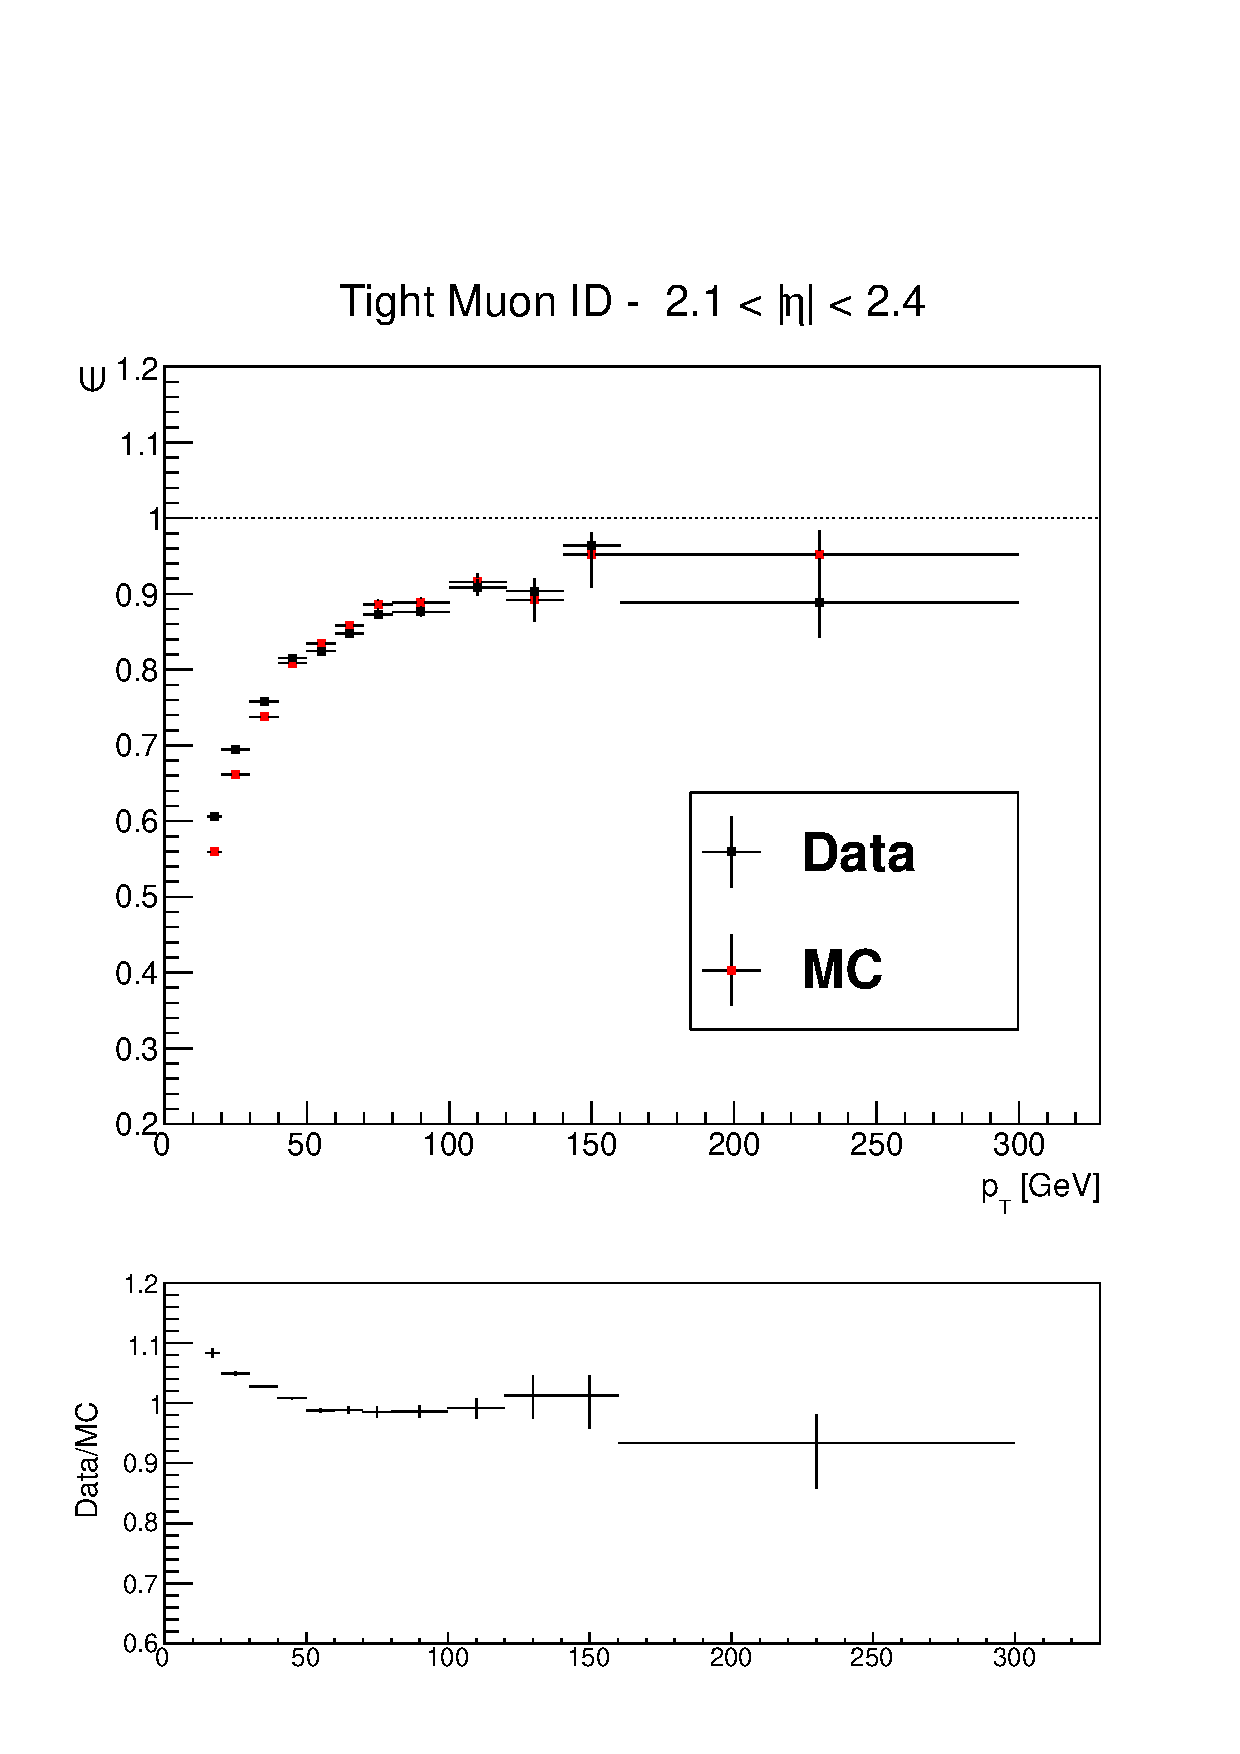
\includegraphics[scale=0.37]{figures/Ch_3_Selection/TagAndProbe/3PassId.pdf}
% 			\par\end{centering}
% 			\caption[Muon Efficiencies using the Tag and Probe method for $\eta$ 1.2 -- 2.4]{\label{fig:DataMC_eta1}Muon Efficiencies using the Tag and Probe method for $|\eta|$ 1.2 -- 2.4.}
% 		\end{figure}
% 		%%%%%%%%%%%%%%%%%%%%%%%%%%%%%%%%%%%%%%%%%%%%%%%%%%%%%%%%%%%%%%%%%%%%%%%%%%%%%%%%%%%%%%%%%

% 		\begin{table}
% 			\caption{Tag and Probe Muon ID efficiencies for MC and data, $\eta$ region 1 and 2.}
% 			\label{table:TPmuon1}
% 			\begin{center}
% 				\begin{tabular*}{\textwidth}{@{\extracolsep{\fill}}cc ccc }\hline
% 					$|\eta|$			& p$_\text{T}$ range (GeV/c) & Data              		& MC                			& Data/MC\\
% 					\hline

% 					$ < 0.9$			& $15 - 20$		& $ 0.556 \pm 0.002 $ 	& $ 0.595 \pm 0.003 $ 	& $ 0.935 \pm 0.005 $\\
% 									& $20 - 30$		& $ 0.672 \pm 0.001 $ 	& $ 0.698 \pm 0.001 $ 	& $ 0.962 \pm 0.001 $\\
% 									& $30 - 40$		& $ 0.755 \pm 0.000 $ 	& $ 0.785 \pm 0.000 $ 	& $ 0.962 \pm 0.001 $\\
% 									& $40 - 50$		& $ 0.821 \pm 0.000 $ 	& $ 0.860 \pm 0.000 $ 	& $ 0.955 \pm 0.000 $\\
% 									& $50 - 60$		& $ 0.851 \pm 0.001 $ 	& $ 0.871 \pm 0.001 $ 	& $ 0.977 \pm 0.001 $\\
% 									& $60 - 70$		& $ 0.869 \pm 0.001 $ 	& $ 0.889 \pm 0.001 $ 	& $ 0.977 \pm 0.002 $\\
% 									& $70 - 80$		& $ 0.886 \pm 0.001 $ 	& $ 0.906 \pm 0.002 $ 	& $ 0.978 \pm 0.002 $\\
% 									& $80 - 100$		& $ 0.895 \pm 0.002 $ 	& $ 0.916 \pm 0.002 $ 	& $ 0.977 \pm 0.003 $\\
% 									& $100 - 120$		& $ 0.906 \pm 0.003 $ 	& $ 0.920 \pm 0.003 $ 	& $ 0.985 \pm 0.004 $\\
% 									& $120 - 140$		& $ 0.917 \pm 0.004 $ 	& $ 0.923 \pm 0.004 $ 	& $ 0.993 \pm 0.006 $\\
% 									& $140 - 160$		& $ 0.929 \pm 0.005 $ 	& $ 0.933 \pm 0.006 $ 	& $ 0.995 \pm 0.008 $\\
% 									& $160 - 300$		& $ 0.916 \pm 0.005 $ 	& $ 0.937 \pm 0.005 $ 	& $ 0.977 \pm 0.007 $\\
% 					\hline
% 					$  0.9 - 1.2$		& $15 - 20$		& $ 0.596 \pm 0.003 $ 	& $ 0.642 \pm 0.003 $ 	& $ 0.929 \pm 0.006 $\\
% 									& $20 - 30$		& $ 0.709 \pm 0.001 $ 	& $ 0.731 \pm 0.001 $ 	& $ 0.970 \pm 0.002 $\\
% 									& $30 - 40$		& $ 0.783 \pm 0.001 $ 	& $ 0.804 \pm 0.001 $ 	& $ 0.973 \pm 0.001 $\\
% 									& $40 - 50$		& $ 0.848 \pm 0.000 $ 	& $ 0.856 \pm 0.001 $ 	& $ 0.991 \pm 0.001 $\\
% 									& $50 - 60$		& $ 0.869 \pm 0.001 $ 	& $ 0.886 \pm 0.001 $ 	& $ 0.981 \pm 0.002 $\\
% 									& $60 - 70$		& $ 0.878 \pm 0.002 $ 	& $ 0.900 \pm 0.002 $ 	& $ 0.976 \pm 0.003 $\\
% 									& $70 - 80$		& $ 0.893 \pm 0.002 $ 	& $ 0.912 \pm 0.003 $ 	& $ 0.980 \pm 0.004 $\\
% 									& $80 - 100$		& $ 0.906 \pm 0.003 $ 	& $ 0.918 \pm 0.003 $ 	& $ 0.987 \pm 0.005 $\\
% 									& $100 - 120$		& $ 0.897 \pm 0.005 $ 	& $ 0.929 \pm 0.005 $ 	& $ 0.966 \pm 0.008 $\\
% 									& $120 - 140$		& $ 0.937 \pm 0.007 $ 	& $ 0.933 \pm 0.008 $ 	& $ 1.005 \pm 0.011 $\\
% 									& $140 - 160$		& $ 0.911 \pm 0.012 $ 	& $ 0.931 \pm 0.011 $ 	& $ 0.978 \pm 0.017 $\\
% 									& $160 - 300$		& $ 0.937 \pm 0.008 $ 	& $ 0.931 \pm 0.010 $ 	& $ 1.006 \pm 0.014 $\\
% 					\hline
% 				\end{tabular*}
% 				\begin{tablenotes}
% 					\item	Note: Errors are statistical only.
% 				\end{tablenotes}
% 			\end{center}
% 		\end{table}
% 		\begin{table}
% 			\caption{Tag and Probe Muon ID efficiencies for MC and data, $\eta$ region 3 and 4.}
% 			\label{table:TPmuon2}
% 			\begin{center}
% 				\begin{tabular*}{\textwidth}{@{\extracolsep{\fill}}cc ccc }\hline
% 					$|\eta|$			& p$_\text{T}$ range (GeV/c) & Data              		& MC                			& Data/MC\\
% 					\hline
% 					$ 1.2 - 2.1$		& $15 - 20$		& $ 0.645 \pm 0.002 $ 	& $ 0.667 \pm 0.002 $ 	& $ 0.967 \pm 0.003 $\\
% 									& $20 - 30$		& $ 0.733 \pm 0.001 $ 	& $ 0.747 \pm 0.001 $ 	& $ 0.981 \pm 0.001 $\\
% 									& $30 - 40$		& $ 0.800 \pm 0.000 $ 	& $ 0.814 \pm 0.001 $ 	& $ 0.983 \pm 0.001 $\\
% 									& $40 - 50$		& $ 0.855 \pm 0.000 $ 	& $ 0.866 \pm 0.000 $ 	& $ 0.987 \pm 0.001 $\\
% 									& $50 - 60$		& $ 0.870 \pm 0.001 $ 	& $ 0.885 \pm 0.001 $ 	& $ 0.983 \pm 0.001 $\\
% 									& $60 - 70$		& $ 0.882 \pm 0.001 $ 	& $ 0.892 \pm 0.001 $ 	& $ 0.990 \pm 0.002 $\\
% 									& $70 - 80$		& $ 0.893 \pm 0.002 $ 	& $ 0.904 \pm 0.002 $ 	& $ 0.987 \pm 0.003 $\\
% 									& $80 - 100$		& $ 0.896 \pm 0.002 $ 	& $ 0.911 \pm 0.002 $ 	& $ 0.983 \pm 0.003 $\\
% 									& $100 - 120$		& $ 0.909 \pm 0.004 $ 	& $ 0.917 \pm 0.004 $ 	& $ 0.991 \pm 0.005 $\\
% 									& $120 - 140$		& $ 0.914 \pm 0.005 $ 	& $ 0.920 \pm 0.006 $ 	& $ 0.994 \pm 0.008 $\\
% 									& $140 - 160$		& $ 0.906 \pm 0.008 $ 	& $ 0.916 \pm 0.008 $ 	& $ 0.989 \pm 0.013 $\\
% 									& $160 - 300$		& $ 0.910 \pm 0.007 $ 	& $ 0.914 \pm 0.008 $ 	& $ 0.996 \pm 0.012 $\\
% 					\hline
% 					$ 2.1 - 2.4$		& $15 - 20$		& $ 0.606 \pm 0.003 $ 	& $ 0.559 \pm 0.003 $ 	& $ 1.083 \pm 0.008 $\\
% 									& $20 - 30$		& $ 0.695 \pm 0.001 $ 	& $ 0.662 \pm 0.001 $ 	& $ 1.049 \pm 0.003 $\\
% 									& $30 - 40$		& $ 0.758 \pm 0.001 $ 	& $ 0.738 \pm 0.001 $ 	& $ 1.028 \pm 0.002 $\\
% 									& $40 - 50$		& $ 0.815 \pm 0.001 $ 	& $ 0.809 \pm 0.001 $ 	& $ 1.008 \pm 0.002 $\\
% 									& $50 - 60$		& $ 0.824 \pm 0.002 $ 	& $ 0.835 \pm 0.002 $ 	& $ 0.988 \pm 0.003 $\\
% 									& $60 - 70$		& $ 0.848 \pm 0.003 $ 	& $ 0.858 \pm 0.004 $ 	& $ 0.988 \pm 0.006 $\\
% 									& $70 - 80$		& $ 0.873 \pm 0.005 $ 	& $ 0.886 \pm 0.006 $ 	& $ 0.985 \pm 0.009 $\\
% 									& $80 - 100$		& $ 0.876 \pm 0.006 $ 	& $ 0.889 \pm 0.007 $ 	& $ 0.986 \pm 0.010 $\\
% 									& $100 - 120$		& $ 0.909 \pm 0.010 $ 	& $ 0.916 \pm 0.012 $ 	& $ 0.992 \pm 0.017 $\\
% 									& $120 - 140$		& $ 0.904 \pm 0.018 $ 	& $ 0.892 \pm 0.026 $ 	& $ 1.013 \pm 0.036 $\\
% 									& $140 - 160$		& $ 0.964 \pm 0.022 $ 	& $ 0.952 \pm 0.035 $ 	& $ 1.013 \pm 0.044 $\\
% 									& $160 - 300$		& $ 0.889 \pm 0.041 $ 	& $ 0.952 \pm 0.045 $ 	& $ 0.933 \pm 0.062 $\\
% 					\hline
% 				\end{tabular*}
% 				\begin{tablenotes}
% 					\item	Note: Errors are statistical only.
% 				\end{tablenotes}
% 			\end{center}
% 		\end{table}




% \section{Background Estimation}\label{bkg}
% 	The main backgrounds in this analysis concern events in which either one muon is fake (e.g. $t \bar t$ and $W$+jets) or both muons are fake (e.g. QCD multijet events).  In the former case, one muon originates from a $W$ decay and is a real prompt muon, while the second muon comes from a jet (likely a $b$ jet, though these muons are typically less isolated).  In the latter case, both muons come from jets and are both non-prompt \textit{fake} muons.

% 	To handle the background estimation, a data driven method is used, referred to as the \textit{fake rate method}, described shortly in Section \ref{sec:fake}.

% 	Monte Carlo simulations generally are not a reliable tool to estimate the fake background, due to the inexact modeling of the parton showering process along with the low probability of getting a jet to `fake' a muon in MC.

% 	As an initial check, Monte Carlo samples are analyzed using the event signature of two same-sign muons and two jets\footnote{Only the preselection criteria are used in order to retain as many events for statistical value.} (Section \ref{section:preselection}) in order to estimate the fake rate, within an order of magnitude.

% 	Using the selections described in Section \ref{section:preselection}, the fake background is found to be comprised of 60\% QCD multijet production, 30\% $W$+~jets, and 15\% $t \bar{t}$. (The last two backgrounds are a much smaller fraction of the total fake background for the final signal selection because of the cuts on MET and the $b$-tag veto.)\footnote{Sources of real same-sign dimuon events in the Standard Model are also considered. This `irreducible' background consists of diboson events ($WZ$, $ZZ$), same-sign $WW$, triboson $WWW$ or $ZZZ$, and $t \bar t$ plus boson ($t \bar t W$, $t \bar t Z$, $t \bar t WW$). These processes have very small cross sections, making their contributions well below that of the background from fakes. They are also estimated using Monte Carlo samples.}$^,$\footnote{The background from muon charge mis-measurement is also considered and found to be negligible.}

% 	\subsection{The Fake Rate Method}\label{sec:fake}

% 		The \textit{fake rate} method is used to estimate the background due to fake muons. The fake rate method is detailed in Reference \cite{fr_method} and has been used in previous analyses; see for example Reference \cite{AN2012-289}.  A very basic description of the method will now be reviewed.

% 		An independent data sample dominated by QCD jets representing the measurement region is used to calculate a fake rate (referred to as the tight-to-loose ratio or T/L ratio).  The fake rate is defined as the fraction of muon candidates passing loose cuts that also pass the tight cuts used in the analysis to select the final event sample:
% 		%
% 		\begin{equation}
% 			FR(\text{p}_\text{T},\eta) = \frac{\#~of~muons~passing~loose~and~tight~selection~criteria}{\#~of~muons~passing~loose~selection~criteria}
% 		\end{equation}
% 		%
% 		Muon candidates that pass the loose cuts are referred to as ``fakeable objects''. The fake rate is calculated as a function of the fakeable object's transverse momentum (p$_\text{T}$) and pseudorapidity ($\eta$). The fake rate is then used as an event weight to calculate the background using a sample of events which pass all the signal selection cuts, except that one or both muons fail the tight selection. This sample is referred to as the ``orthogonal'' sample.

% 		An estimate of the fake rate prediction is obtained by weighting each event in which one muon passes the tight cuts and the other muon fails the tight selection but passes the loose selection ($N_{n\bar{n}}$) and the number of events in which both muons fail the tight selection but pass the loose cuts ($N_{\bar{n}\bar{n}}$). The total contribution to the signal sample (in other words the number of events in which both muons pass the tight selection, ($N_{nn}$), is obtained by summing all the weighted events as in Equation \ref{eq:FR_equation}.

% 		A simplified version of the method is implemented, assuming that the probability for a real prompt muon to pass the tight selection is 1. This assumption simplifies the method and reduces possible sources of systematic errors\footnote{Even if a very tight ID is used, the contamination coming from same-sign prompt events (like $WZ$) in the orthogonal sample is on the order of 1\% of the total number of events with one tight and one loose muon.  As such it is not necessary to apply a correction for a contamination this small.}.

% 		The equations that relate the number of events with prompt-prompt ($N_{pp}$), prompt-fake ($N_{pf}$), and fake-fake($N_{ff}$) muons to $N_{n\bar{n}}$, $N_{\bar{n}\bar{n}}$, and  $N_{nn}$ are:
% 		\begin{equation} \label{eq:FR_equation1}
% 				N_{tot} = N_{pp} + N_{pf} + N_{ff} 	= N_{n n} + N_{n\bar{n}} + N_{\bar{n}\bar{n}}\\
% 		\end{equation}
% 		\begin{equation} \label{eq:FR_equation2}
% 		    		N^{ij}_{\bar{n}\bar{n}}			= (1-FR_i)(1-FR_j)  N^{ij}_{ff} \\
% 		\end{equation}
% 		\begin{equation} \label{eq:FR_equation3}
% 		    		N^{ij}_{n\bar{n}}				= (1-FRj)  N^{ij}_{pf} + (FR_i (1-FR_j) + FR_j (1-FR_i)) N^{ij}_{ff} \\
% 		\end{equation}
% 		\begin{equation} \label{eq:FR_equation4}
% 		        		N^{ij}_{n n}					= N^{ij}_{pp} + FR_j N^{ij}_{pf} + FR_i FR_j  N^{ij}_{ff}
% 		\end{equation}

% 		After some quick algebra, the fake contribution to the signal sample $N_{nn}$ can be derived to:
% 		%
% 		\begin{multline}\label{eq:FR_equation}
% 			N_{nn} = \sum_{i,j} { \frac{FR_i \; FR_j}{(1-FR_i)(1-FR_j)} N_{\bar{n}\bar{n}}^{ij}} \\
% 		       + \sum_{i,j} \frac{FR_i}{(1-FR_i)} \left[ N_{n\bar{n}}^{ij} -  \frac{FR_i(1 - FR_j) + FR_j(1 - FR_i)}{(1 - FR_i) (1 - FR_j)}  N_{\bar n \bar n}^{ij} \right]
% 		\end{multline}
% 		%
% 		where $FR$ is the fake rate, and $i,j$ label the two muons in the event. Note that in the square parentheses we have explicitly written the correction to $N^{ij}_{n \bar n}$ due to $\bar n \bar n$ events that can be also be $n \bar n$. In the hypothesis of no real sources of events with two prompt leptons, this term has to be identically zero as all the single fake events must be generated from double fake events (double-to-single).

% 	\subsection{Fake Rate Measurement in Data}
% 		\textit{Fakeable} objects are defined by relaxing the muon ID requirements. The following loose cuts are used to select fakeable muons:
% 		\begin{itemize}
% 			\item $\chi^2/number~of~degrees~of~freedom$ (analysis cut $<10$, loose selection $<50$);
% 			\item Transverse impact parameter $d_{xy}$ (analysis cut $<0.05$ mm, loose selection $<2$ mm);
% 			\item $RelIso$ (analysis cut $<0.05$, loose selection $<0.4$).
% 		\end{itemize}
% 		Fakeable objects are defined as muon candidates passing the selection defined in \ref{subsec:muonSelection}, but with these three cuts relaxed.

% 		The independent control sample used to obtain the fake rate is selected using the following single muon triggers:
% 		\begin{itemize}
% 			\item {\tt HLT\_Mu8}
% 			\item {\tt HLT\_Mu12}
% 			\item {\tt HLT\_Mu17}
% 			\item {\tt HLT\_Mu24}
% 		\end{itemize}

% 		\noindent
% 		The first two triggers are used for the p$_\text{T}$ bin $10 <$ p$_\text{T} \le 20$ GeV/$c$, the third for $20 < $p$_\text{T} \le 25$ GeV/$c$, and the last for p$_\text{T}$ bins above 25 GeV/$c$.

% 		The goal is to measure the fake rate in QCD events.  By definition there are no tight muons in QCD events. Therefore, dijet-like events are selected. The selected events must contain one muon that passes the loose requirements (probe) and one jet (tag) on the opposite side to the muon ($\Delta \phi_{\mu j} > 2.5$, as dijets are generally distributed) that satisfies the same selection cuts used in the analysis except for the p$_\text{T}$ requirement, which in this case is set at p$_\text{T} > 40$ GeV/$c$. (This p$_\text{T}$ cut is chosen to match the expected p$_\text{T}$ distribution of the fake objects in the orthogonal sample as shown in Figure \ref{fig:fake_pt}, which reflects the distribution expected in the signal region.  More on Figure \ref{fig:fake_pt} in Section \ref{FRvalidation}.)

% 		\begin{figure}
% 			\begin{center}
% 				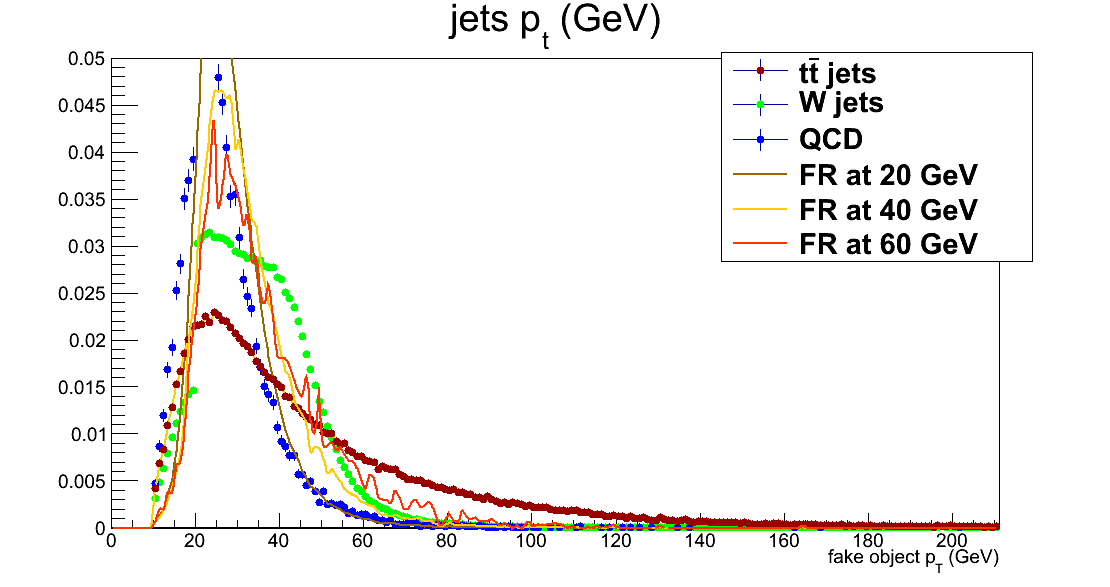
\includegraphics[width=15cm]{figures/Ch_3_Background/fake_pt.png}
% 				\caption[The p$_\text{T}$ spectrum of jets tagged as a fake object in MC.]{The p$_\text{T}$ spectrum of jets tagged as a fake object in MC.  Comparison between $t\bar{t}$, $W+jets$, and QCD Monte Carlo. The shapes are normalized to unity.}
% 				\label{fig:fake_pt}
% 			\end{center}
% 		\end{figure}

% 		In order to reject $W$ events, the cuts MET $< 20$ GeV and transverse mass $M_T < 25$ GeV/$c^2$ are imposed.  To suppress $Z$ events, a veto is applied to events with more than one muon. Dimuon events are checked using the full $M_T$ spectrum to check the normalization of the Drell-Yan and $W$~+~jets MC, after being normalized to the trigger luminosities of the four triggers, in what can be defined as a fake rate control region. Events with an invariant mass $m_{\mu\mu}$ within 20 GeV/$c^2$ of the $Z$ boson mass are only used to check the normalization of the Drell-Yan Monte Carlo (see Figure \ref{fig:fakerate_mll}). The normalization of the $W$~+~jets Monte Carlo is checked in the large $M_T$ region (Figure \ref{fig:fakerate_MT}).
% 		%
% 		\begin{figure}
% 			\begin{center}
% 				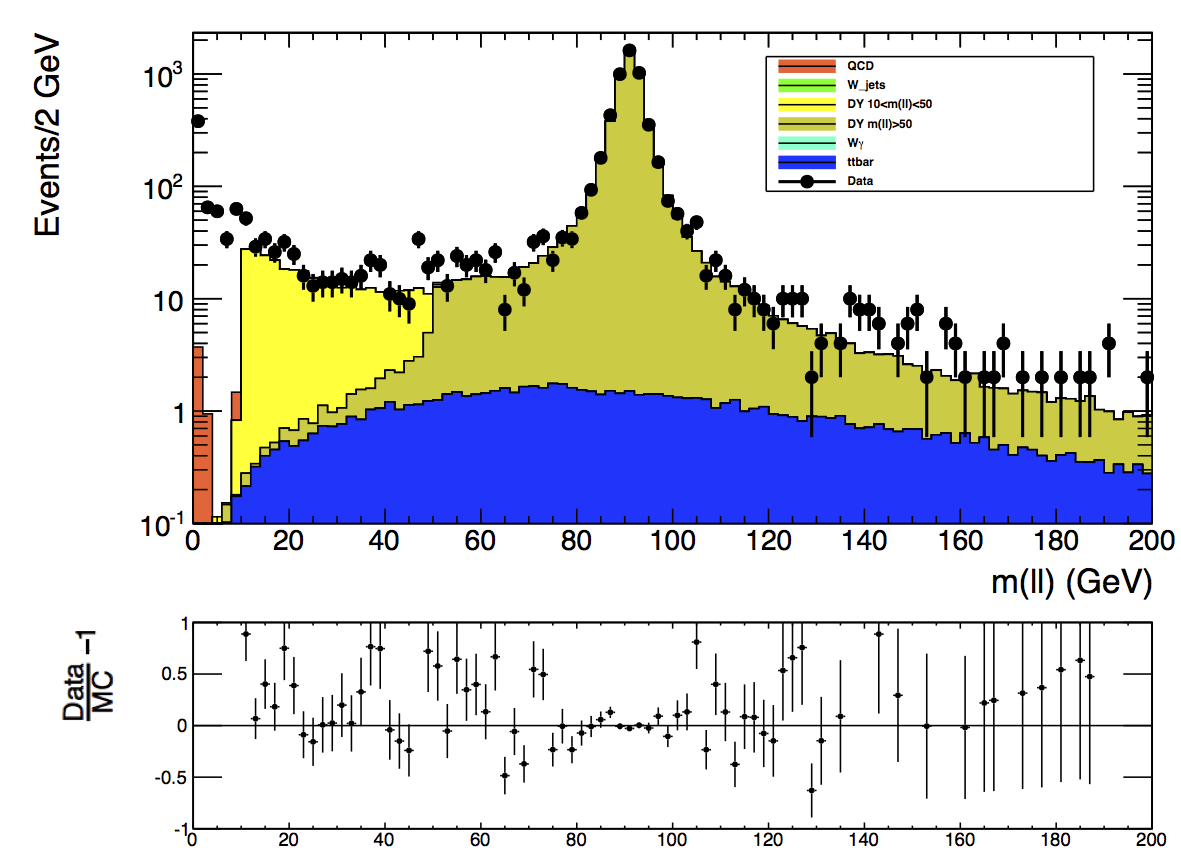
\includegraphics[width=12cm]{figures/Ch_3_Background/h_mll.png}
% 				\caption[The $m(ll)$ distribution of the events in the fake-rate control region.]{The $m(ll)$ distribution of the events in the fake-rate control region. The invariant mass, $m(ll)$, is calculated using the two leading leptons and requiring one jet above 40 GeV/c.}
% 				\label{fig:fakerate_mll}
% 			\end{center}
% 		\end{figure}
% 		%
% 		\begin{figure}
% 			\begin{center}
% 				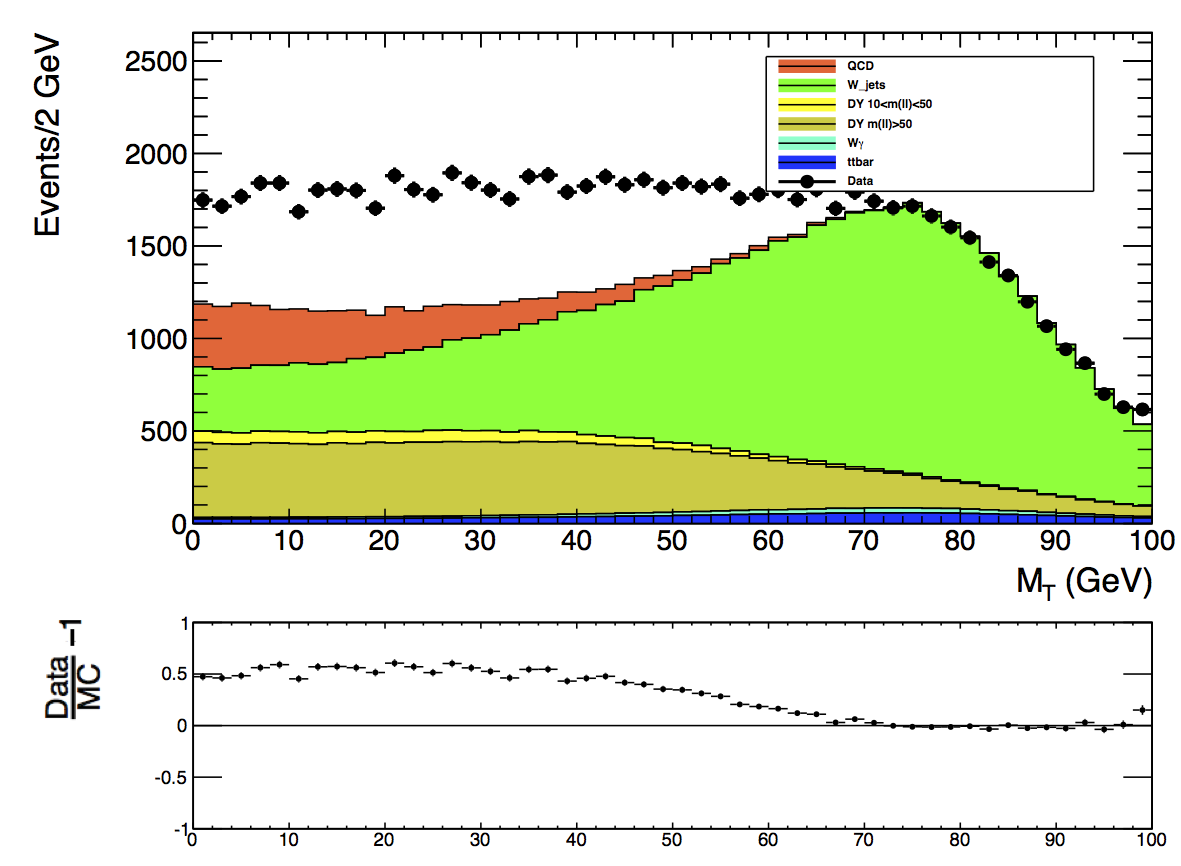
\includegraphics[width=12cm]{figures/Ch_3_Background/h_MT.png}
% 				\caption[The transverse mass ($M_T$) distribution of the events in the fake-rate control region.]{The transverse mass ($M_T$) distribution of the events in the fake-rate control region. $M_T$ is calculated using the leading lepton and requiring one jet above 40 GeV/c. The lack of events at small $M_T$ is due to lack of Monte Carlo events in the QCD sample.}
% 				\label{fig:fakerate_MT}
% 			\end{center}
% 		\end{figure}

% 		The fake rate is corrected for any remaining prompt contamination by subtracting the Monte Carlo contributions of $W$, $Z$,  $t \bar t$  and $W\gamma$ processes from both the numerator (tight) and denominator (loose).  The distributions of p$_\text{T}$ and $\eta$ for the events in the numerator and denominator selections are plotted in Figures \ref{fig:num_den_plots_pT} and \ref{fig:num_den_plots_eta}.
% 		%
% 		\begin{figure}
% 			\begin{center}
% 				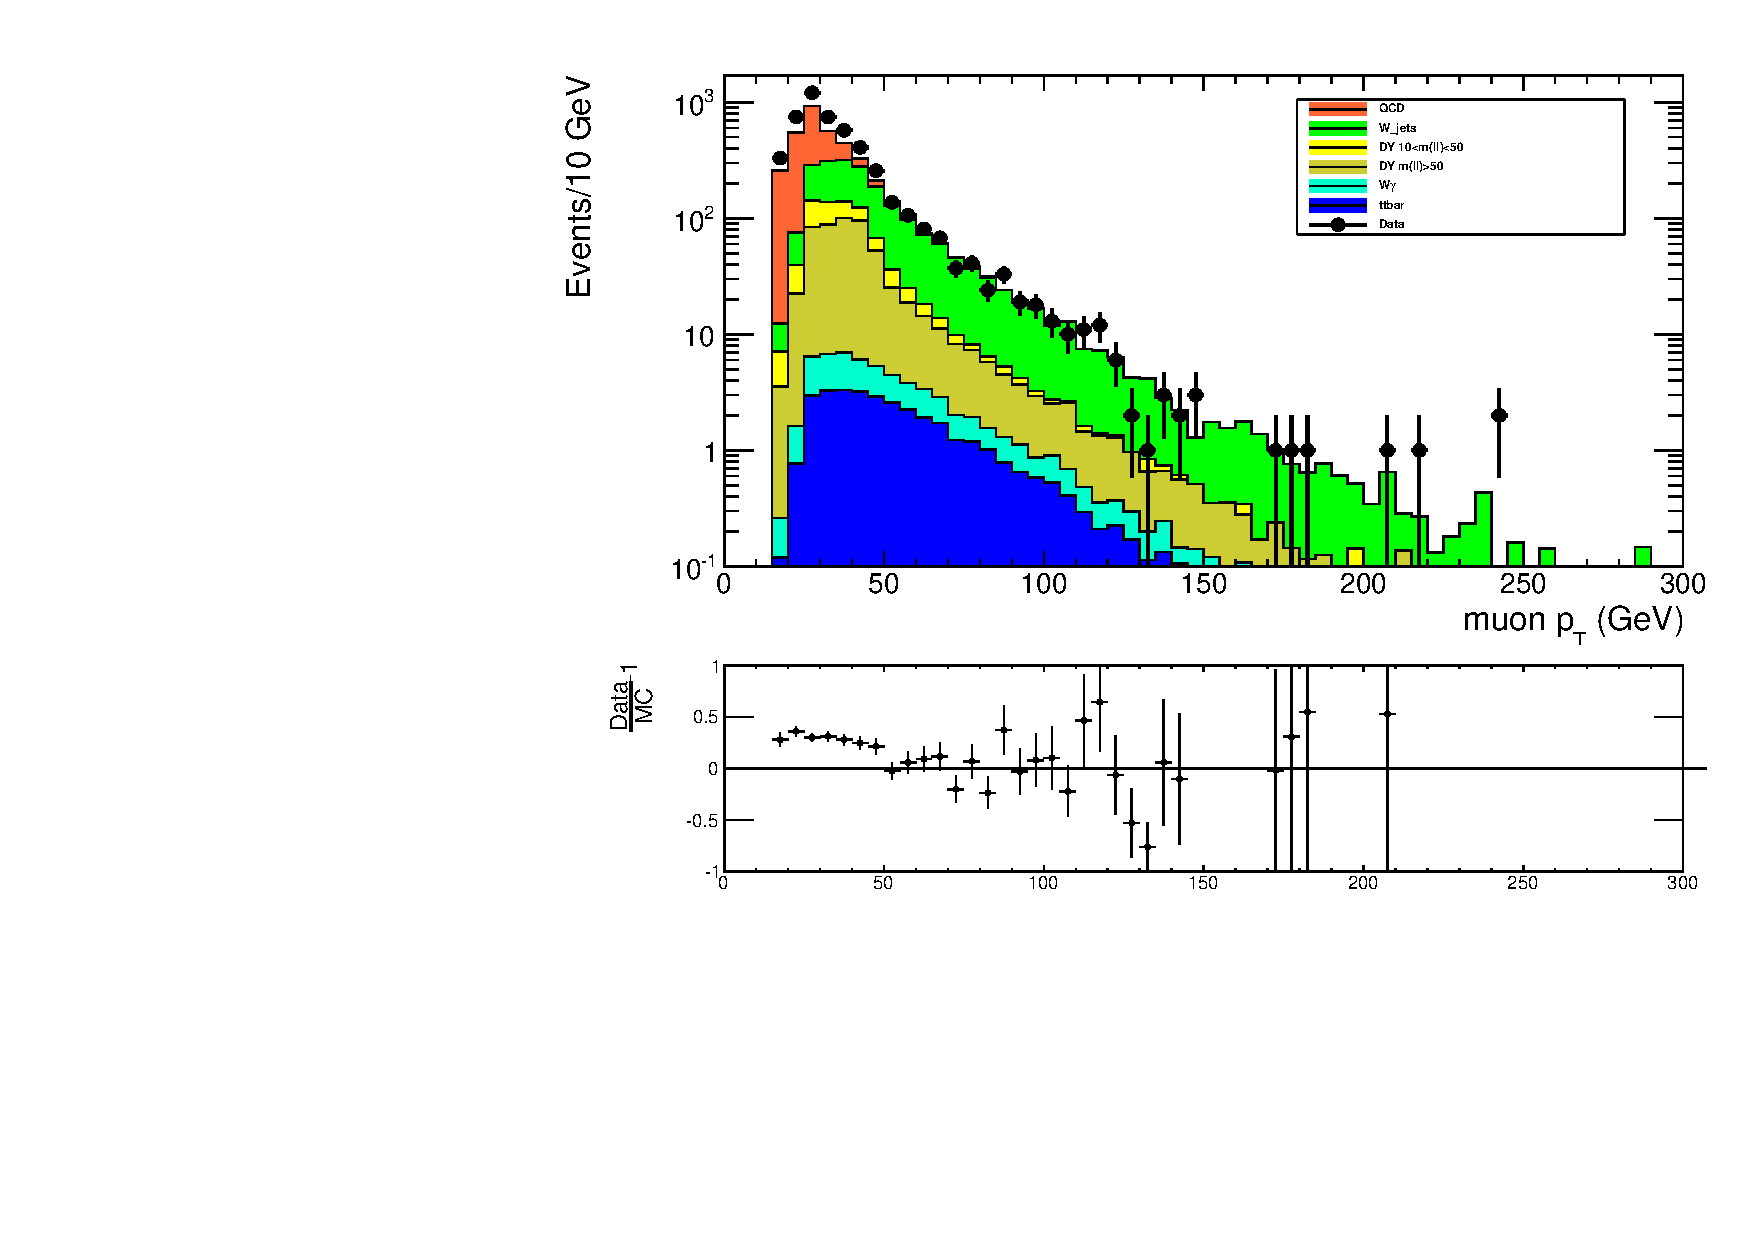
\includegraphics[width=14cm]{figures/Ch_3_Background/h_TL_numerator_pt_log.pdf}
% 				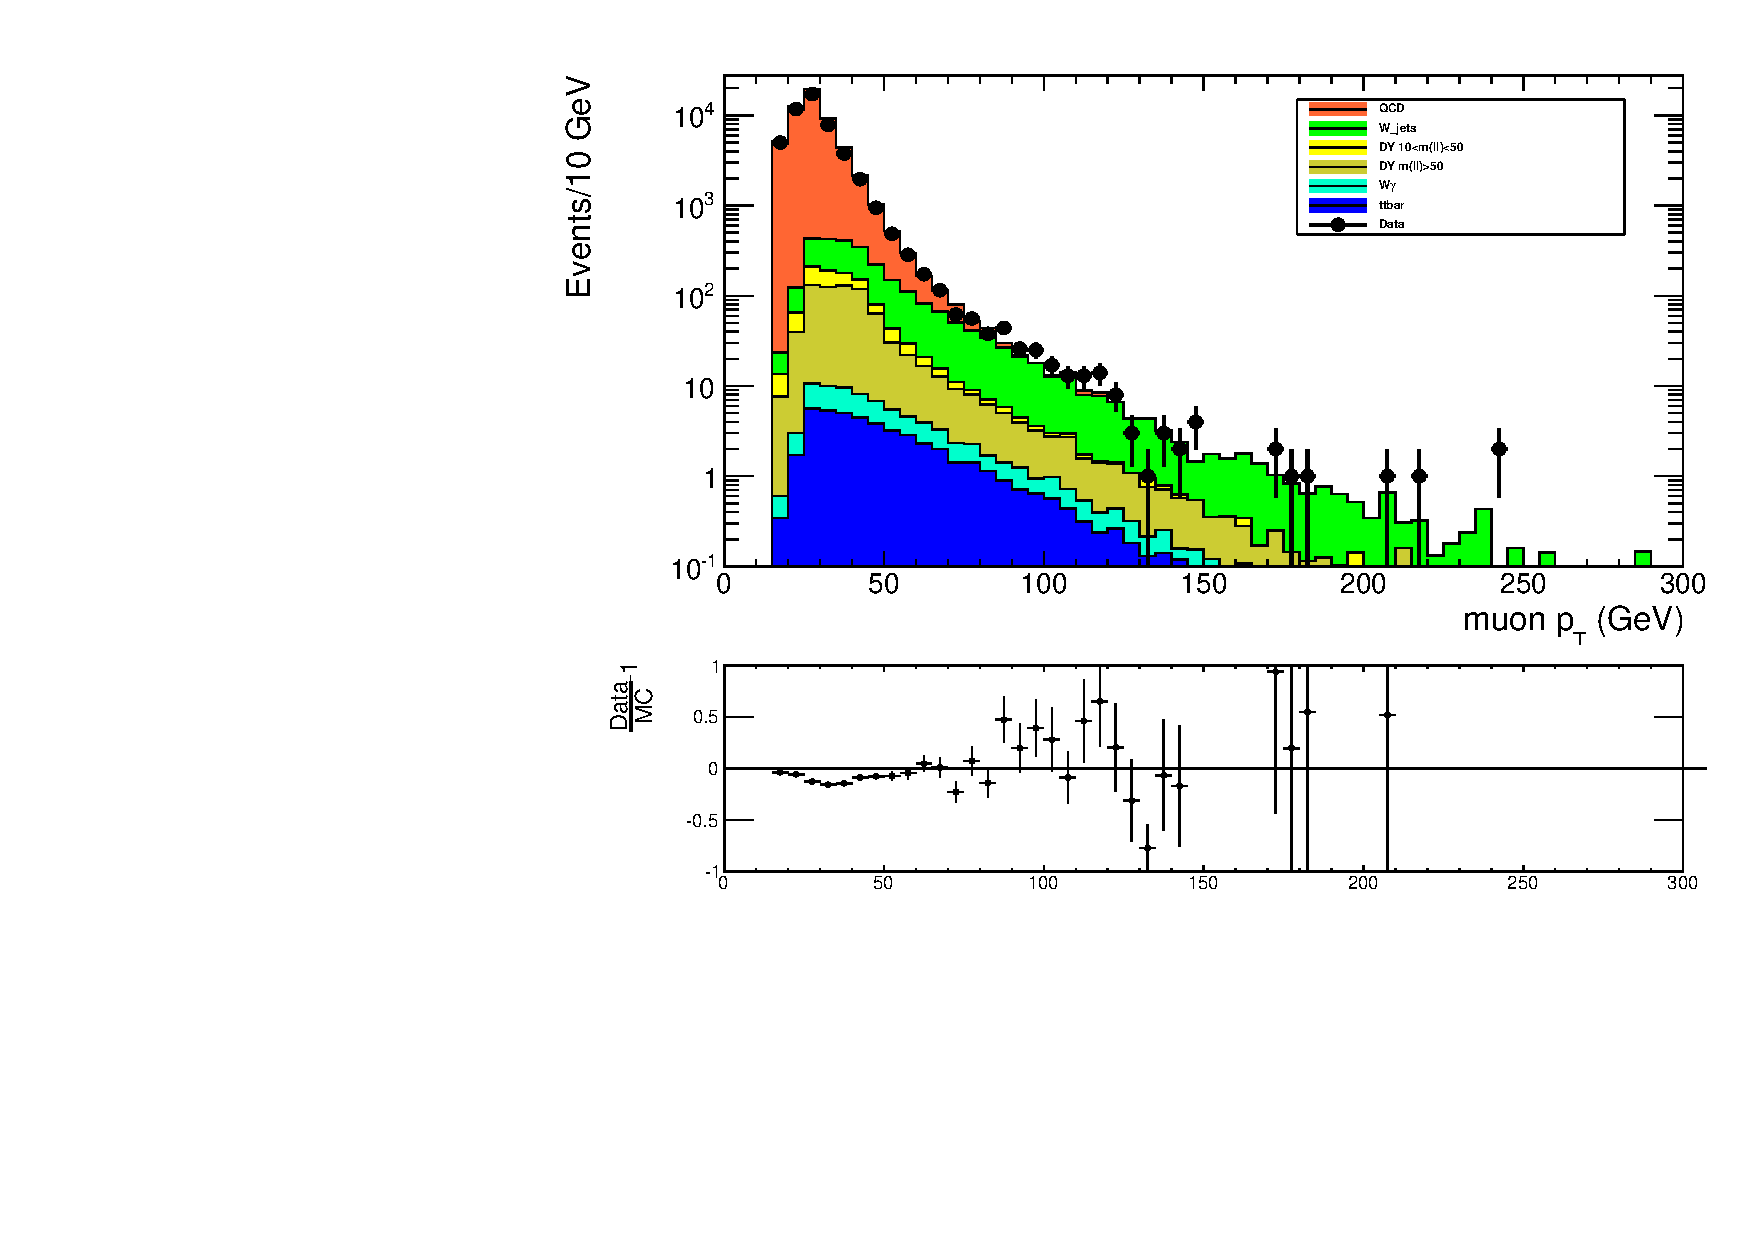
\includegraphics[width=14cm]{figures/Ch_3_Background/h_TL_denominator_pt_log.pdf}
% 				\caption{$p_T$ distributions for the tight muons (top) and loose muons (bottom) used in the fake rate calculation.}
% 				\label{fig:num_den_plots_pT}
% 			\end{center}
% 		\end{figure}

% 		\begin{figure}
% 			\begin{center}
% 				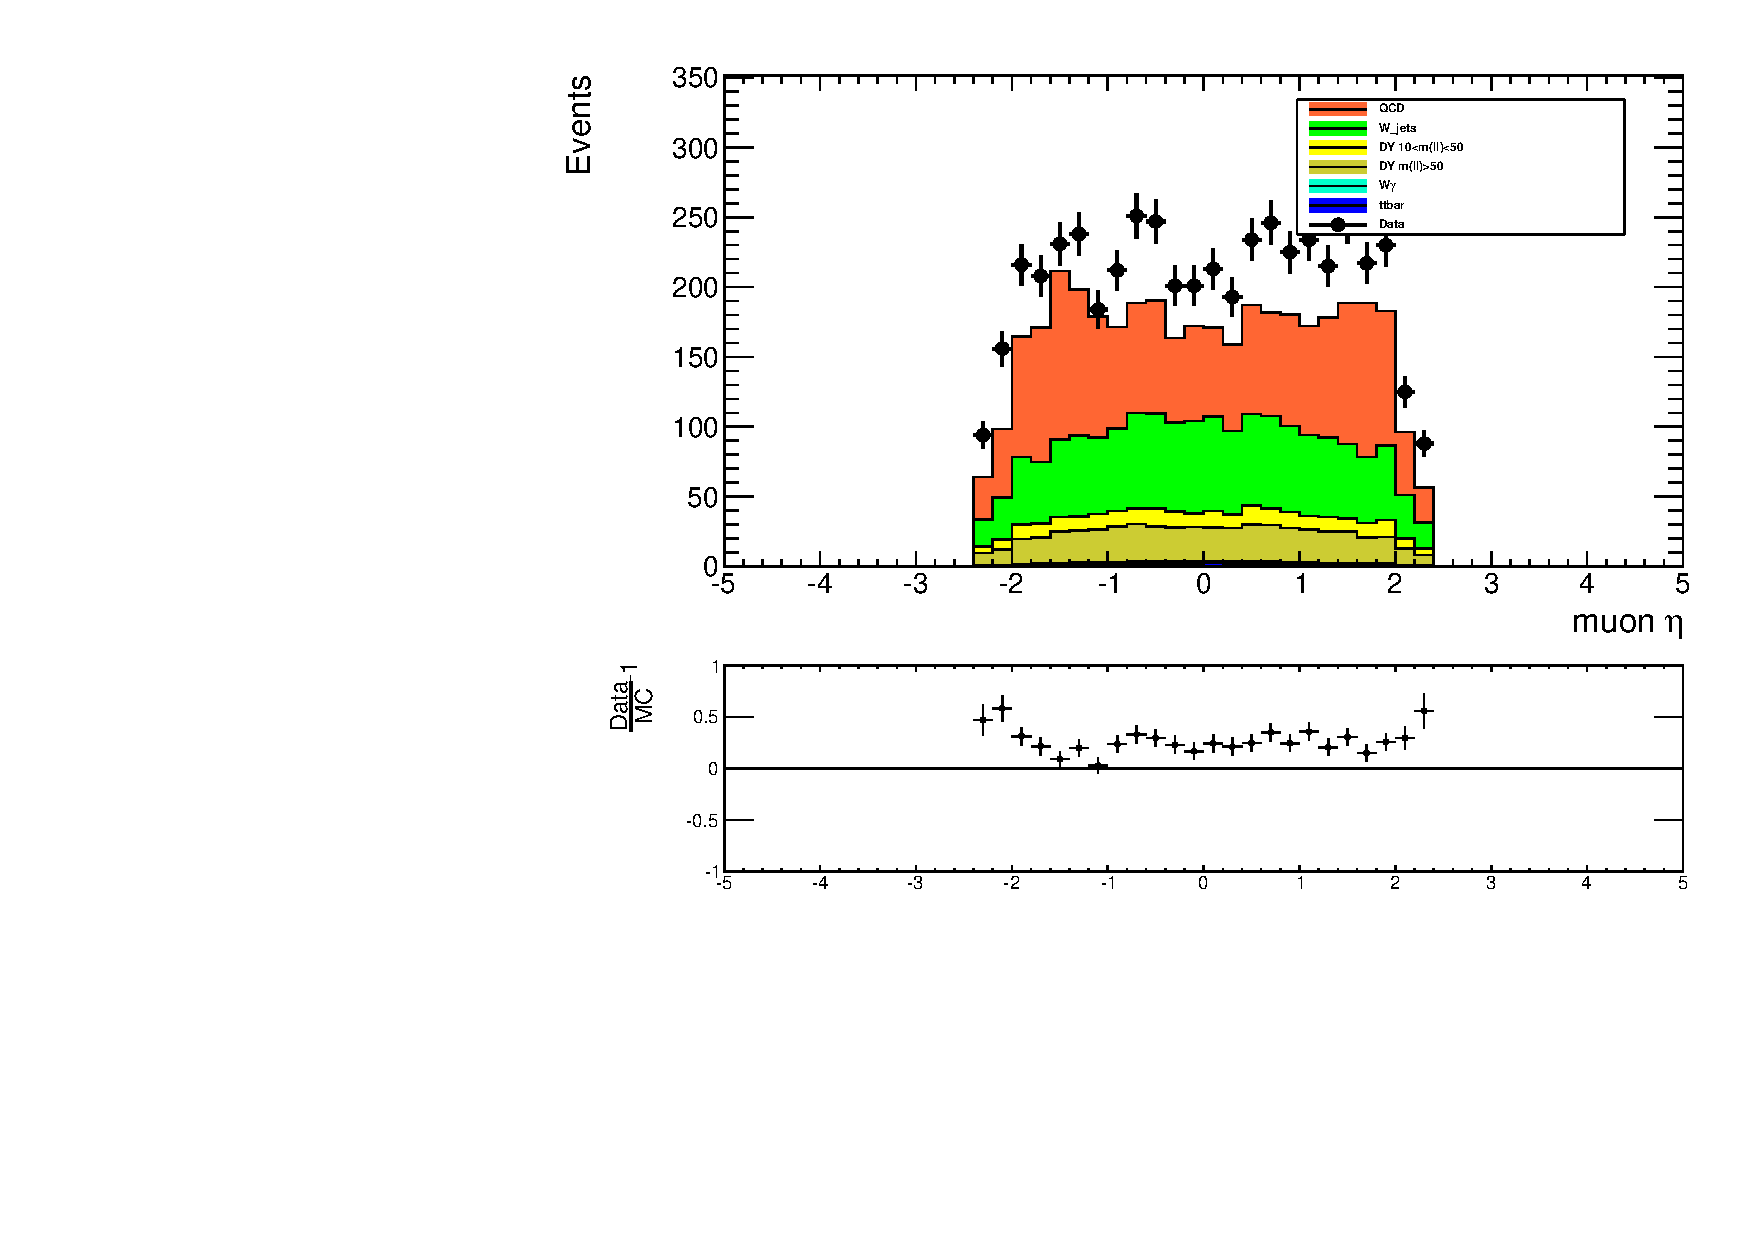
\includegraphics[width=14cm]{figures/Ch_3_Background/h_TL_numerator_eta.pdf}
% 				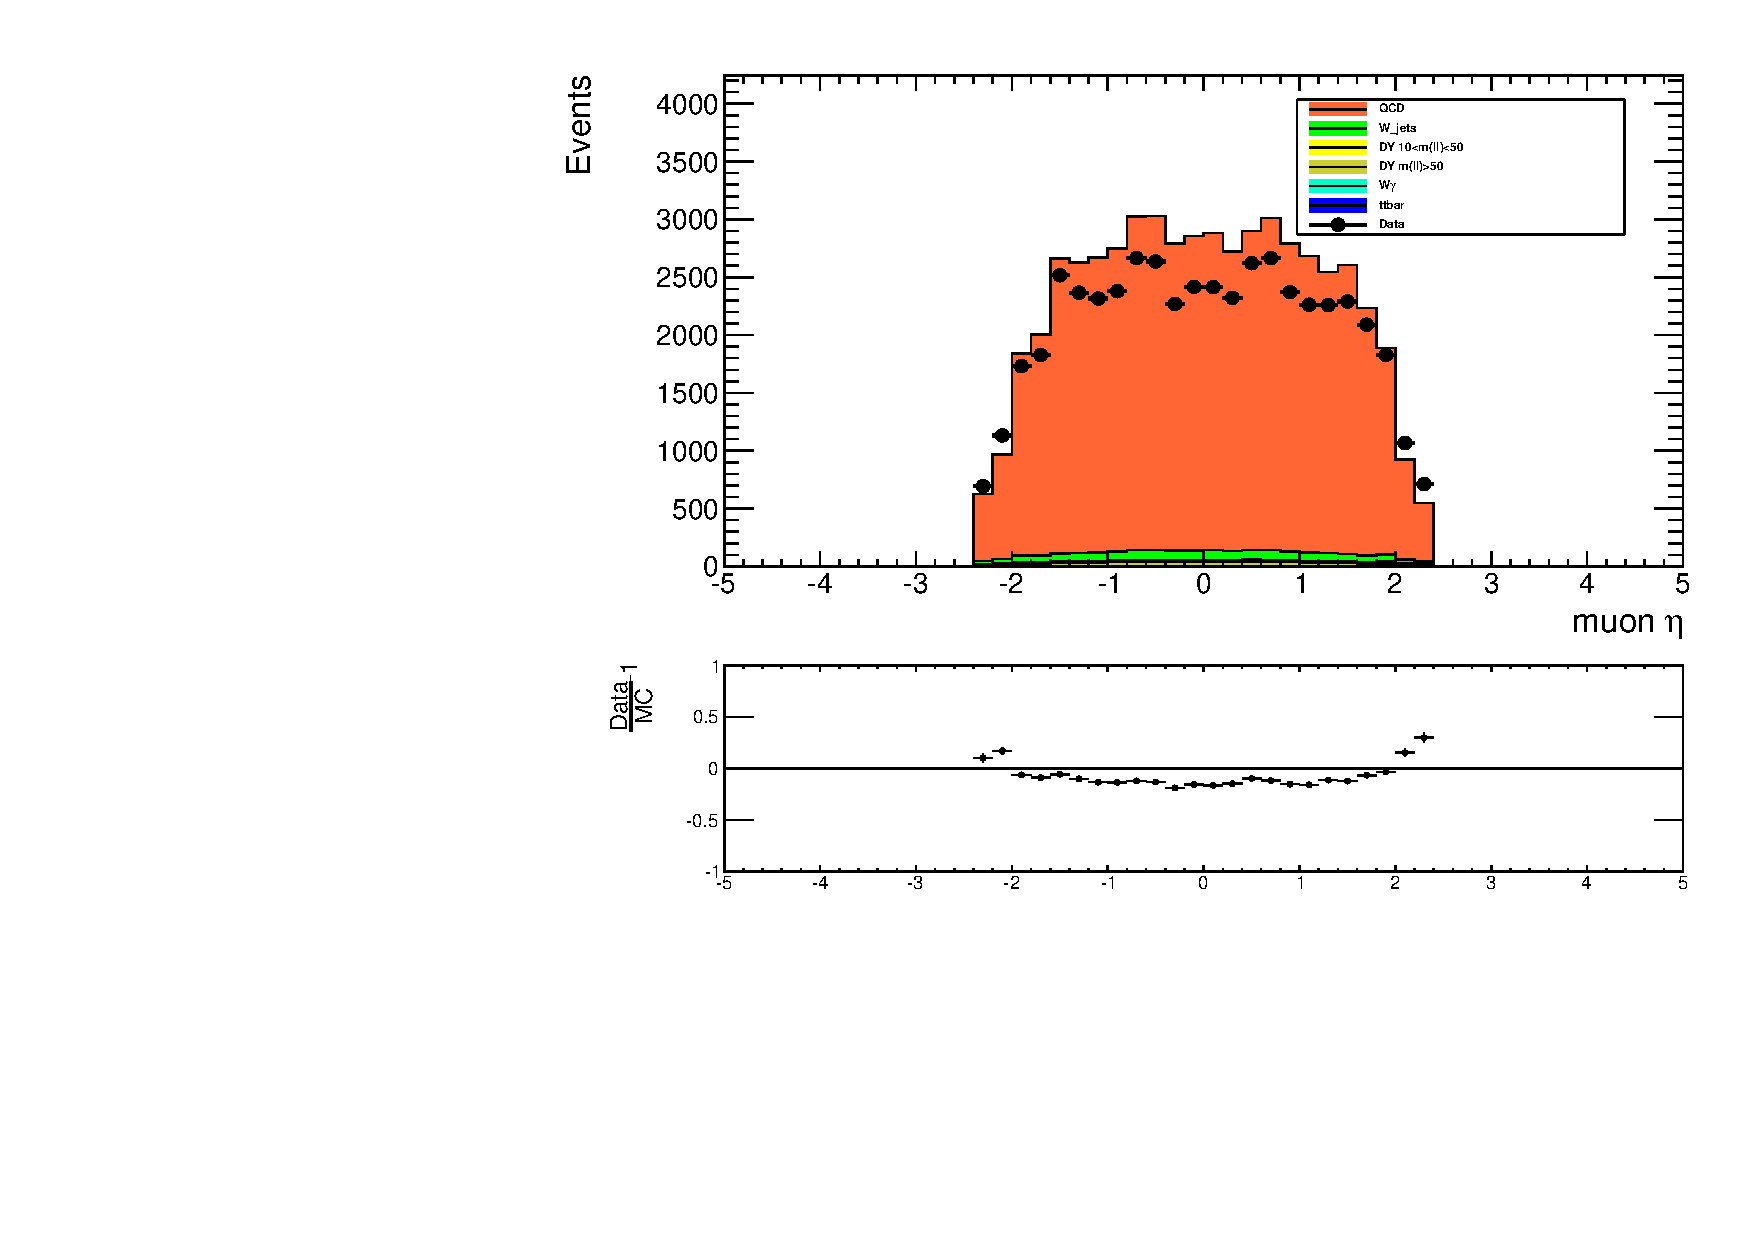
\includegraphics[width=14cm]{figures/Ch_3_Background/h_TL_denominator_eta.pdf}
% 				\caption{$\eta$ distributions for the tight muons (top) and loose muons (bottom) used in the fake rate calculation.}
% 				\label{fig:num_den_plots_eta}
% 			\end{center}
% 		\end{figure}


% 		The fake rates obtained, (including the Monte Carlo subtraction), are listed in Table \ref{table:mu_fr} and are plotted in Figure \ref{fig:mu_fr_2dplot}. Since electroweak processes become dominant with increasing muon p$_\text{T}$, a flat fake rate for p$_\text{T} > 60$ GeV/$c$ is assumed, using the numbers listed in the 45 -- 60 GeV/$c$ row in Table \ref{table:mu_fr}.
% 		%
% 		\begin{table}
% 			\caption{Muon fake rates obtained from data in bins of $|\eta|$ and p$_\text{T}$.}
% 			\label{table:mu_fr}
% 			\begin{center}
% 				\begin{tabular}{c|cccccc}
% 				\hline
% 				p$_\text{T}$ Range			& \multicolumn{4}{c}{$|\eta|$ Region}\\
% 				 (GeV/c)				&	0 -- 0.8			&	0.8 -- 1.479		&	1.479 -- 2.0		&	2.0 -- 2.5\\
% 				\hline
% 				15-20				&	$0.052 \pm 0.007$	&	$0.060 \pm 0.008$	&	$0.080 \pm 0.011$	&	$0.089 \pm 0.005$\\
% 				20-25				&	$0.050 \pm 0.004$	&	$0.050 \pm 0.005$	&	$0.079 \pm 0.007$	&	$0.070 \pm 0.012$\\
% 				25-30				&	$0.044 \pm 0.004$	&	$0.051 \pm 0.004$	&	$0.071 \pm 0.006$	&	$0.091 \pm 0.013$\\
% 				30-35				&	$0.044 \pm 0.004$	&	$0.066 \pm 0.008$	&	$0.068 \pm 0.010$	&	$0.080 \pm 0.019$\\
% 				35-45				&	$0.067 \pm 0.011$	&	$0.070 \pm 0.013$	&	$0.106 \pm 0.019$	&	$0.077 \pm 0.031$\\
% 				45-60				&	$0.076 \pm 0.032$	&	$0.058 \pm 0.039$	&	$0.027 \pm 0.039$	&	$0.231 \pm 0.117$\\

% 				\hline
% 				\end{tabular}
% 			\end{center}
% 		\end{table}
% 		%
% 		\begin{figure}[tbph]
% 		\begin{center}
% 			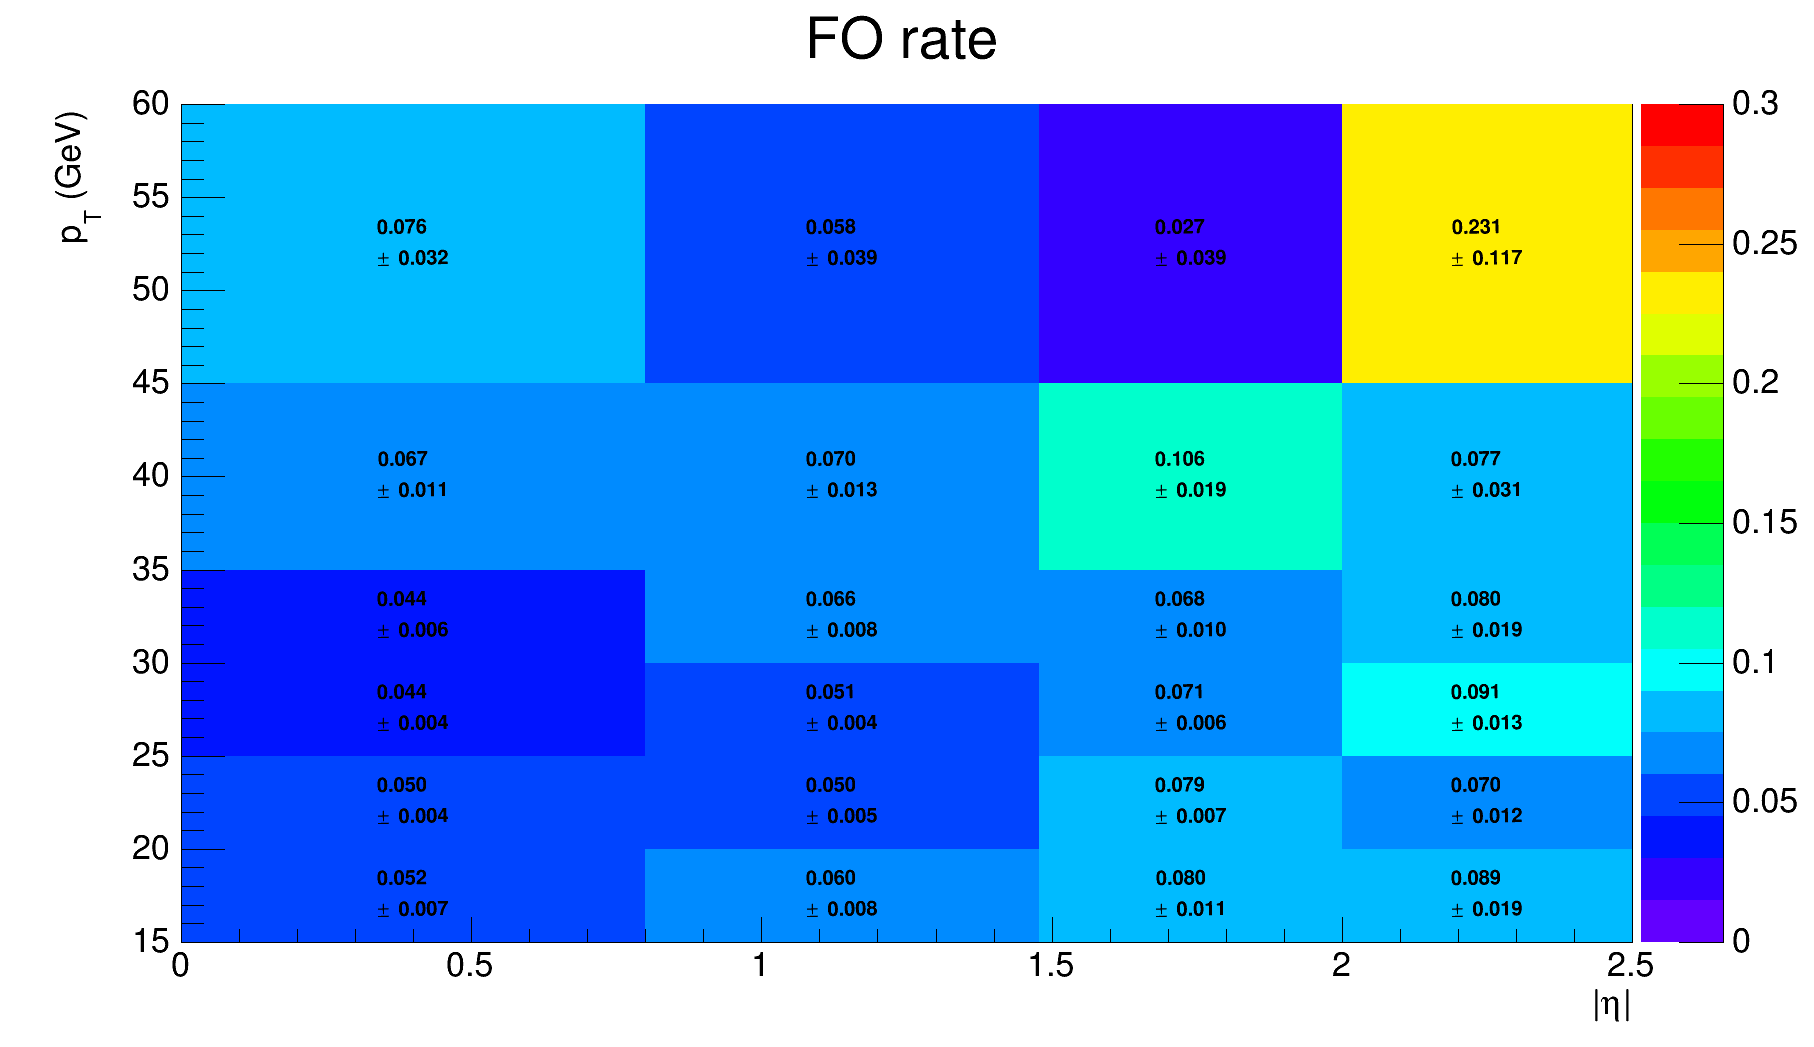
\includegraphics[width=15cm]{figures/Ch_3_Background/FR-map.png}
% 			\caption{Muon fake rates obtained from data as a function of $\eta$ and p$_\text{T}$.}
% 			\label{fig:mu_fr_2dplot}
% 		\end{center}
% 		\end{figure}


% 	\subsection{Validation of the Fake Rate Method}\label{FRvalidation}
% 		The fake rate method is evaluated by testing it on Monte Carlo samples in which the true background from fakes can be determined. The fake rates are obtained from a sample of muon enriched MC QCD multijet events, and are used to estimate the fake backgrounds in Monte Carlo $t \bar t$, $W$~+~jets, and QCD multijet events.

% 		The predicted background depends on the choice of the p$_\text{T}$ cut on the leading jet in the sample used to measure the fake rates.  Figure \ref{fig:fake_pt} compares the p$_\text{T}$ distribution of the fakeable objects in QCD, $W$~+~jets, and  $t \bar t$ events with the p$_\text{T}$ of the fakeable objects in the independent QCD sample used to calculate the fake rates with different cuts on the leading jet p$_\text{T}$ in the latter sample. The first three samples, plotted as dots in Figure \ref{fig:fake_pt}, share the analysis preselection (Section \ref{section:preselection}) but with inverted isolation requirements on the muons to pick events with loose muons and nearby jets. If two loose muons with two nearby jets are present in the event, two entries are added to the histogram. The QCD sample, plotted with different p$_\text{T}$ cuts on the away-side jet, instead uses the same selection as used for the fake rate measurement sample to select the jet near the loose (denominator) object.

% 		A cut of p$_\text{T} > 40$ GeV/c is used in the final calculation of the fake rate as this choice roughly matches the p$_\text{T}$ of the fakeable objects from which the fake rates are calculated to the fakeable objects in the $t \bar t$, $W$~+~jets, and QCD multijet samples. The p$_\text{T}$ distribution of the jet generating the loose muon must not be misinterpreted as the p$_\text{T}$ of the loose muon. For instance, consider a $t \bar{t}$ event in which a $b$-quark hadronizes, producing a loose muon.  The p$_\text{T}$ of the loose muon will be correlated to the initial p$_\text{T}$ of the $b$ but it won't be the same.  Furthermore, the energy of the generated particle also affects the isolation of the loose object. Matching the p$_\text{T}$ of the generating particles in the fake rate measurement region and application region improves the level of agreement between prediction and observation in the closure tests.

% 		Table \ref{table:mu_closure_l} summarizes the results of the validation of the fake rate method for events passing the loose selection. The same selection as used to select signal events is applied, except for the MET cut. For the QCD sample the same-sign requirement is also relaxed in order to increase the statistics. For $t \bar t$, the predicted background is overestimated by 50\%\footnote{The overestimate in the case of $t \bar t$ is also observed in the same-sign SUSY analysis \cite{SUSY_2010, SUSY_2011} and is attributed to the harder p$_\text{T}$ distribution of fakeable objects in $t \bar t$ events compared to the $p_T$ distribution in the independent QCD sample used to calculate the fake rates. The overestimate decreases to 23\% when the p$_\text{T}$ cut is raised to 80 GeV/$c$.}. The prediction for $W$~+~jets is in agreement with the true fake background and is within the uncertainty of roughly 10\%, while for QCD the agreement is also reasonable with an uncertainty of 24\%.

% 		For QCD events, an additional test of the fake rate method is performed by counting the number of tight to loose events ($N_{n \bar n}$) in the MC sample and is compared with the predicted number obtained from the number of loose-loose events ($N_{\bar n \bar n}$) scaled by the corresponding fake rate factors. The results of this test (the last row of Table \ref{table:mu_closure_l}) shows that the prediction is good to within 14\%.
% 		%
% 		\begin{table}
% 			\caption[Predicted (\#FR) and observed (\#MC) fake backgrounds in $t \bar t$, $W$~+~jets, and QCD Monte Carlo samples for events passing preselection.]{Predicted (\#FR) and observed (\#MC) fake backgrounds in $t \bar t$, $W$~+~jets, and QCD Monte Carlo samples for events passing preselection.}
% 			\label{table:mu_closure_l}
% 			\begin{center}
% 				\begin{tabular*}{\textwidth}{@{\extracolsep{\fill}}ccccc}
% 					\hline
% 					Sample 				& $p_T$ Cut (GeV/c)& \# FR 			& \# MC		& \% diff. \\
% 					\hline
% 					$t \bar t$ 				& 40  			& $46.3 \pm 1.5 $    	& $23$   		& $50.4 \pm 3.2$ \\
% 					$t \bar t$			 	& 60 		 	& $39.8 \pm 1.4 $    	& $23$   		& $42.2 \pm 3.5$\\
% 					$W$~+~jets 			& 40 			& $0.54 \pm 0.17$  	& $1$   		& $84.8\pm 30.6$\\
% 					QCD        				& 40   			& $0.15 \pm 0.12$  	& $0$    		& $n.a.$\\
% 					QCD double-to-single 	& 40  			& $7.01\pm 0.76$  	& $6$   		& $14.4 \pm 10.9$\\
% 					\hline
% 				\end{tabular*}
% 			\end{center}
% 		\end{table}

% 	%\subsection{Systematic Uncertainty on Background Estimate}




% \section{Selection Results}\label{finalSelection}
% 	\subsection{Low Mass Selection Results}
% 		The final background estimates are given in Table \ref{table:mu_yields_l}. The total background estimate is $11.2 \pm 1.1~(stat) \pm 2.1~(syst)$ events, with the dominant contribution being the fake muon background ($8.19 \pm 0.96~(stat) \pm 2.05~(syst)$ events).  The data yield is in good agreement with this estimate (within errors).

% 		After all selection cuts (described in Sections \ref{Section:selectionEfficiency}), and before the final optimization cuts, 7 events were observed in data.
% 		%
% 		\begin{table}
% 			\caption{Observed event yields and estimated backgrounds with statistical and systematic uncertainties for the low mass selection.}
% 			\label{table:mu_yields_l}
% 			\begin{center}
% 				\begin{tabular*}{\textwidth}{@{\extracolsep{\fill}}l  l}
% 					\hline
% 					Source & Events \\
% 					\hline
% 					Monte Carlo:  		& \\
% 					~~$VV$               	& $2.31 \pm 0.37~(stat) \pm 0.35~(syst)$ \\
% 					~~$VVV$               	& $0.12 \pm 0.03~(stat) \pm 0.02~(syst)$ \\
% 					~~$t \bar t V$       	& $0.12 \pm 0.05~(stat) \pm 0.02~(syst)$ \\
% 					Total Monte Carlo    	& $2.55 \pm 0.37~(stat) \pm 0.35~(syst)$ \\
% 					\hline
% 					Data-driven background estimate: 	& \\
% 					Fake muon background 			& $8.19 \pm 0.96~(stat) \pm 2.05~(syst)$ \\
% 					\hline
% 					Total background     				& $10.74 \pm 1.03~(stat) \pm 2.08~(syst)$ \\
% 					\hline
% 					Observed in data (19.7 fb$^{-1}$) & $7$ \\
% 					\hline
% 				\end{tabular*}
% 			\end{center}
% 		\end{table}

% 		\begin{figure}
% 			\begin{center}
% 				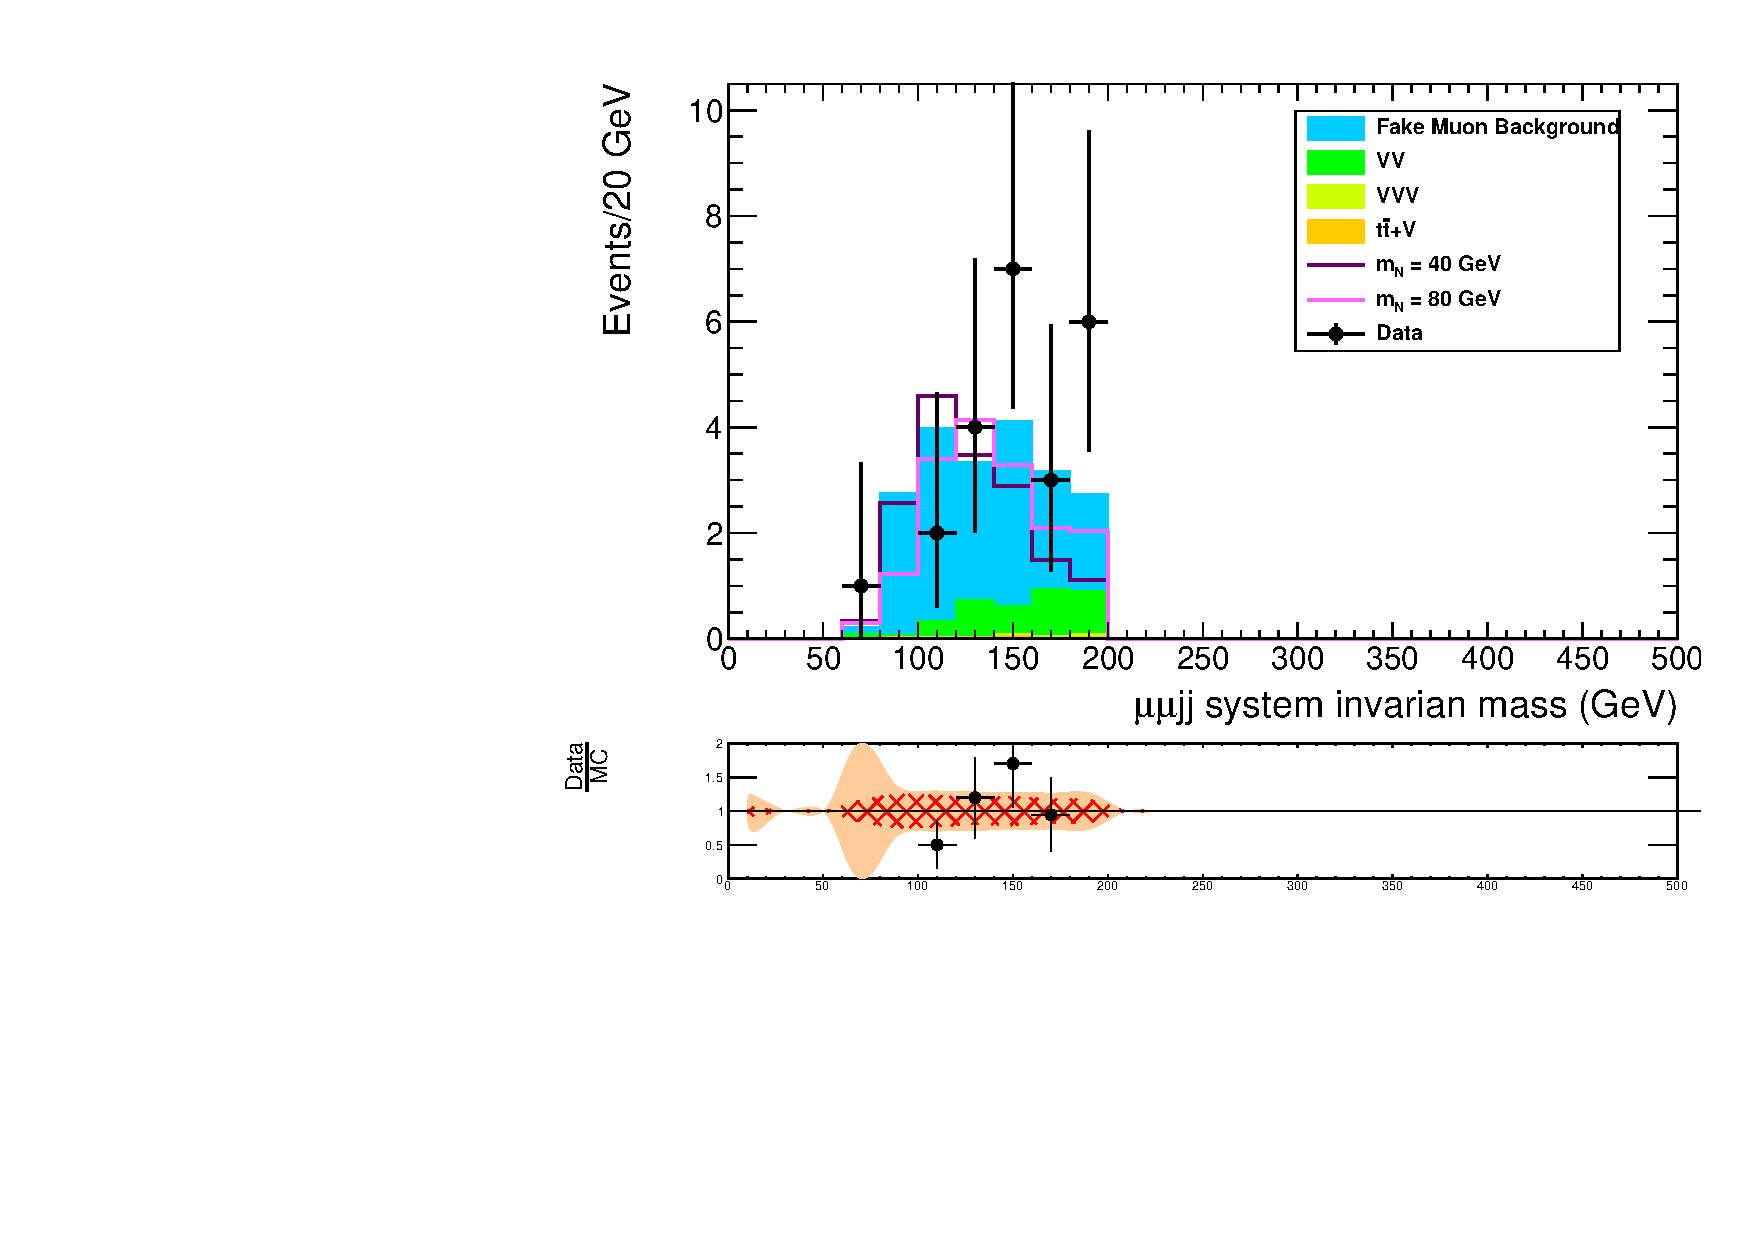
\includegraphics[scale=0.5]{figures/Ch_3_Results/h_lljjmass_.pdf}
% 				\caption[The invariant four-mass ($\mu\mu j j$), for events passing the low mass selection.]{The invariant four-mass ($\mu\mu j j$), for events passing the low mass selection.}
% 				\label{fig:mass_lljj_low}
% 			\end{center}
% 		\end{figure}

% 		The final selection cut optimization is performed on the transverse momenta of the two muons ($p_{T1}$ and $p_{T2}$) and the invariant mass of the two muons and jets $m(\mu \mu j j)$ using the Punzi figure of merit, as described in Section \ref{punziFoM}. The results from the low mass region optimization are listed in Table~\ref{tab:opt_low}.
% 		%
% 		\begin{table}
% 			\centering
% 			\caption{Results of the cut optimization for the low mass Majorana neutrino region.}
% 			\label{tab:opt_low}
% 			\begin{center}
% 				\begin{tabular*}{\textwidth}{@{\extracolsep{\fill}}ccccccccc}
% 				\hline
% 				$N_R$ Mass 	& $m(\mu \mu j j)$  	& $p_{T1}$  	& $p_{T2}$ 				& Tot. Bkgd. 	& Eff. 		& $N_{obs}$ \\
% 				(GeV/$c^2$) 	& (GeV/$c^2$) 		&  (GeV/$c$)  	& (GeV/$c$) 				& 			& (\%) 		& \\
% 				\hline
% 				40 			& 80 			& 20			& 15					  	& 9.28 $\pm$ 0.97  	& 0.78 	& 7 \\
% 				50 			& 80 			& 20 		& 15					  	& 9.28 $\pm$ 0.97  	& 0.90  	& 7 \\
% 				60  			& 80 			& 20 		& 15					  	& 9.28 $\pm$ 0.97  	& 0.73  	& 7 \\
% 				70 			& 90 			& 20 		& 15					  	& 8.63 $\pm$ 0.92  	& 0.29  	& 7 \\
% 				80 			& 100			& 20 		& 15					  	& 7.84 $\pm$ 0.82  	& 1.21  	& 7 \\
% 				\hline
% 				\end{tabular*}
% 			\end{center}
% 		\end{table}

% 	\subsection{High Mass Selection Results}
% 	The final background estimates are given in Table \ref{table:mu_yields_t}. The total background estimate is $22.8 \pm 1.4$ (stat) $\pm 3.6$ (syst) events, with the dominant contribution arising from the fake muon background ($13.6 \pm 1.2$ (stat) $\pm 3.4$ (syst) events).

% 	After the application of all selection cuts as defined in Sections \ref{subsec:muonSelection} -- \ref{section:fullselection}, and before the final optimization, 19 events were observed in data.

% 	\begin{table}
% 	\caption{Observed event yields and estimated backgrounds with statistical and systematic uncertainties for the high mass selection.}
% 		\label{table:mu_yields_t}
% 		\begin{center}
% 			\begin{tabular*}{\textwidth}{@{\extracolsep{\fill}}l  l}
% 				\hline
% 				Source & Events \\
% 				\hline
% 				Monte Carlo:  & \\
% 				~~$VV$               	& $7.10 \pm 0.65~(stat) \pm 1.14~(syst)$ \\
% 				~~$VVV$               	& $0.35 \pm 0.05~(stat) \pm 0.06~(syst)$ \\
% 				~~$t \bar t V$       	& $0.32 \pm 0.08~(stat) \pm 0.05~(syst)$ \\
% 				Total Monte Carlo    	& $9.17 \pm 0.80~(stat) \pm 1.26~(syst)$ \\
% 				\hline
% 				Data-driven background estimate: & \\
% 				Fake muon background & $13.62 \pm 1.16~(stat) \pm 3.40~(syst)$ \\
% 				\hline
% 				Total background     & $ 21.39 \pm 1.34~(stat) \pm 3.59~(syst)$ \\
% 				\hline
% 				Observed in data (19.7 fb$^{-1}$) & $19$ \\
% 				\hline
% 			\end{tabular*}
% 		\end{center}
% 	\end{table}

% 	As in the low mass region, the final selection is optimized on the p$_\text{T}$ of the two muons, and the invariant mass of the four mass ($\mu\mu j j$).  The results of the optimization are listed in Table \ref{tab:opt_high}.

% 	\begin{table}
% 		\centering
% 		\caption[Results of the cut optimization for the `high mass' region.]{Results of the cut optimization for the `high mass' region.}
% 		\label{tab:opt_high}
% 		\begin{center}
% 			\begin{tabular*}{0.85\textwidth}{@{\extracolsep{\fill}}ccccccccc}
% 				\hline
% 				HMN & $m(\mu \mu j j)$  & $p_{T1}$, $p_{T2}$ & Tot. Bkgd. & Eff. & $N_{obs}$ \\
% 				GeV/$c^2$	& GeV/$c^2$	&  GeV/$c$	& GeV/$c$  & &\\
% 				\hline
% 				90 	& 120 	& 20, 15	& 19.45 $\pm$ 1.21  & 1.17 	& 19 \\
% 				100 	& 120 	& 20, 15	& 19.45 $\pm$ 1.21  & 4.82  	& 19 \\
% 				125 	& 140 	& 25, 20	& 13.00 $\pm$ 0.94  & 11.18  	& 8 \\
% 				150 	& 160 	& 35, 25	& 9.33 $\pm$ 0.74  	& 13.77  	& 7 \\
% 				175 	& 200 	& 45, 35	& 5.61 $\pm$ 0.58  	& 13.87   	& 5 \\
% 				200 	& 220 	& 55, 35	& 3.74 $\pm$ 0.48  	& 15.86   	& 5 \\
% 				250 	& 270 	& 70, 45	& 1.88 $\pm$ 0.33  	& 16.21 	& 3 \\
% 				300 	& 290 	& 100, 45	& 0.91 $\pm$ 0.25  	& 14.50 	& 1 \\
% 				350 	& 290 	& 100, 45	& 0.91 $\pm$ 0.25  	& 15.50   	& 1 \\
% 				400 	& 290 	& 100, 45	& 0.91 $\pm$ 0.25  	& 15.27 	& 1 \\
% 				500 	& 290 	& 100, 45	& 0.91 $\pm$ 0.25  	& 12.09   	& 1 \\
% 				\hline
% 			\end{tabular*}
% 		\end{center}
% 	\end{table}


% \section{Systematic Uncertainties}\label{systematics}
% 	The mechanics of this search consist mainly of those of a standard counting experiment.  In such an experiment, the dominant sources of systematic uncertainty are due to the process of generating the signal, the efficiencies of the measurement, and prediction of the signal contamination (or \textit{background}).  These uncertainties are standard among CMS searches, and references abound on the mechanics of handling them.  The following sources of systematic uncertainty are taken into account:
% 	%
% 	\begin{itemize}
% 		\item \textit{Integrated Luminosity}:  The systematic uncertainty on the integrated luminosity is 2.6\%, .

% 	  	\item \textit{Parton Distribution Functions}: The ALPGEN signal Monte Carlo parton distribution function uncertainty is estimated using the method in Ref.~\cite{PDFUncert}. The resulting uncertainty is $3.5\%$ of the signal yield.

% 		\item \textit{$Q^2$ Scale}: The $Q^2$ scale parameter in ALPGEN is varied from $Q^2/4$ to $4Q^2$.  The uncertainty ranges from 4\% to 10\% for the low mass region, and 1\% to 7\% at high mass.

% 		\item \textit{Muon Trigger and Selection}: The systematic uncertainty due to the uncertainty in the muon trigger efficiency is taken from the muon POG~\cite{piet_talk}, with a value of 2\%.

% 		\item \textit{Jet Energy Scale}:  The jet energy is scaled by the official energy uncertainty \cite{JetUncert} and the resulting effect on the signal efficiency is observed. The resulting systematic uncertainty is between 3\% to 11\% for the low mass selection, and 1\% to 6\% in the high mass range.

% 		\item \textit{Jet Energy Resolution}: The JER is found to depend on the Majorana Neutrino mass and is found to be 4\% to 12\% for the low mass region and 2\% to 6\% for the high mass region.

% 		\item \textit{Unclustered energy}: Unclustered energy affects the signal efficiency due to the higher MET cut. The uncertainty is below $2\%$ for the low mass region and less than $1\%$ for the high mass region.

% 		\item \textit{b-Tag efficiency and mistag}: The b-tag efficiency and mistag rate are varied independently for heavy and light flavors.  The effect is less than $1\%$.

% 		\item \textit{Pileup Model}: As recommended by the Reference \cite{PU_syst}, the minimum bias cross-section was changed in order to alter the pileup profile. This results in a systematic uncertainty of 6\% to 7\% for the low mass region and 4\% to 6\% for the high mass region..

% 		\item \textit{Background Estimate}: The uncertainty on the fake background is 28\%.  The uncertainty in the normalizations of irreducible SM backgrounds are: 12\% for  $WZ$~\cite{CMS_WZ}; 9\% for $ZZ$~\cite{CMS_ZZ}, 22\% for $WW$~\cite{CMS_ZZ}; and 25\% for the other processes, determined by varying the $Q^2$ scale and parton distribution functions in Monte Carlo simulations.
% 	\end{itemize}

% 	 A summary of the systematic uncertainties is given in Table~\ref{table:mu_sys}.
% 	%
% 	\begin{table}
% 		\caption{Summary of systematic uncertainties.}
% 		\label{table:mu_sys}
% 		\begin{center}
% 			\begin{tabular}{l cccc}
% 				\hline
% 				                     						& \multicolumn{3}{c}{Majorana Neutrino Mass (GeV/$c^2$)}\\
% 				Source               					&40		 &80		&200	&500\\
% 				\hline
% 				~~~Integrated Luminosity              		& 2.60\% 	 & 2.60\% 	& 2.60\%  	& 2.60\%\\
% 				~~~Muon Efficiency                       		& 2.00\%   & 2.00\% 	& 2.00\%  & 2.00\%\\
% 				~~~Jet Energy Scale                   		& 10.48\% & 6.14\% & 1.68\% 	& 0.97\%\\
% 				~~~Jet Energy Resolution              		& 12.05\% & 7.15\%	& 2.94\% 	& 2.26\%\\
% 				~~~Unclustered energy				& 0.92\%   & 1.71\%	& 0.77\% 	& 0.78\%\\
% 				~~~b-Tag efficiency and mistag		& 0.73\%   & 0.75\%	& 0.57\% 	& 0.49\%\\
% 				~~~Pile Up Model                      			& 6.91\%  	 & 7.70\% 	& 4.09\% 	& 3.58\%\\
% 				~~~Parton distribution Functions      		& 3.50\%  	&  3.50\% & 3.50\%	& 3.50\% \\
% 				% Combined
% 				\hline
% 			\end{tabular}
% 		\end{center}
% 	\end{table}



% \section{Interpretation of Results}
% 	There is no excess of events beyond the predicted Standard Model background.  Thus, limits are set on the square of the Majorana neutrino mixing element.  The limits are based on the number of observed events, the number of predicted background events, and the number of predicted events from Majorana neutrino production.  The 95\% confidence level limit on the cross section for heavy Majorana production is obtained using the standard CMS RooStatsCl95 package\cite{rooStats1, rooStats2}, by applying the \textit{CLs} method.  See \cite{cls95} for a very good review of the method.

% 	From this, the 95\% C.L. limit on the mixing element squared can be calculated using the ``bare" cross section defined as the cross section for a mixing of 1.0 obtained from the signal Monte Carlo simulation.

% 	The limits are set on the mixing element squared, $|V_{\mu N}^2|$, which is directly proportional to HMN production cross section.  The limits are set as a function of HMN mass, with the assumption that the mixing elements for electron and tau neutrinos are zero.  Figure \ref{fig:exclusion} shows the limits vs. HMN mass, and Figure \ref{fig:exclusionZoom} shows the same limits zoomed to the mass region 40 -- 200 GeV/$c^2$.

% 	This search is an improvement over previous searches, not only because the limits extend to higher masses than before, but because of the more advanced techniques used to set the limits.  By binning the search into different regions and optimizing the selection variables with a figure of merit, a more sensitive search with tighter limits was able to be performed.  Figure \ref{fig:exclusion} includes the limits set by previous searches, as well as a line labeled \textit{preselection} which shows what the observed limit would be without the final selection optimization as a function of HMN mass, (described in Section \ref{punziFoM}).

% 	%%%%%%%%%%%%%%%%%%%%%%%%%%%%%%%%%%% Exclusion Plot %%%%%%%%%%%%%%%%%%%%%%%%%%%%%%%%%%%%%%%%
% 	\begin{figure}
% 		\begin{centering}
% 			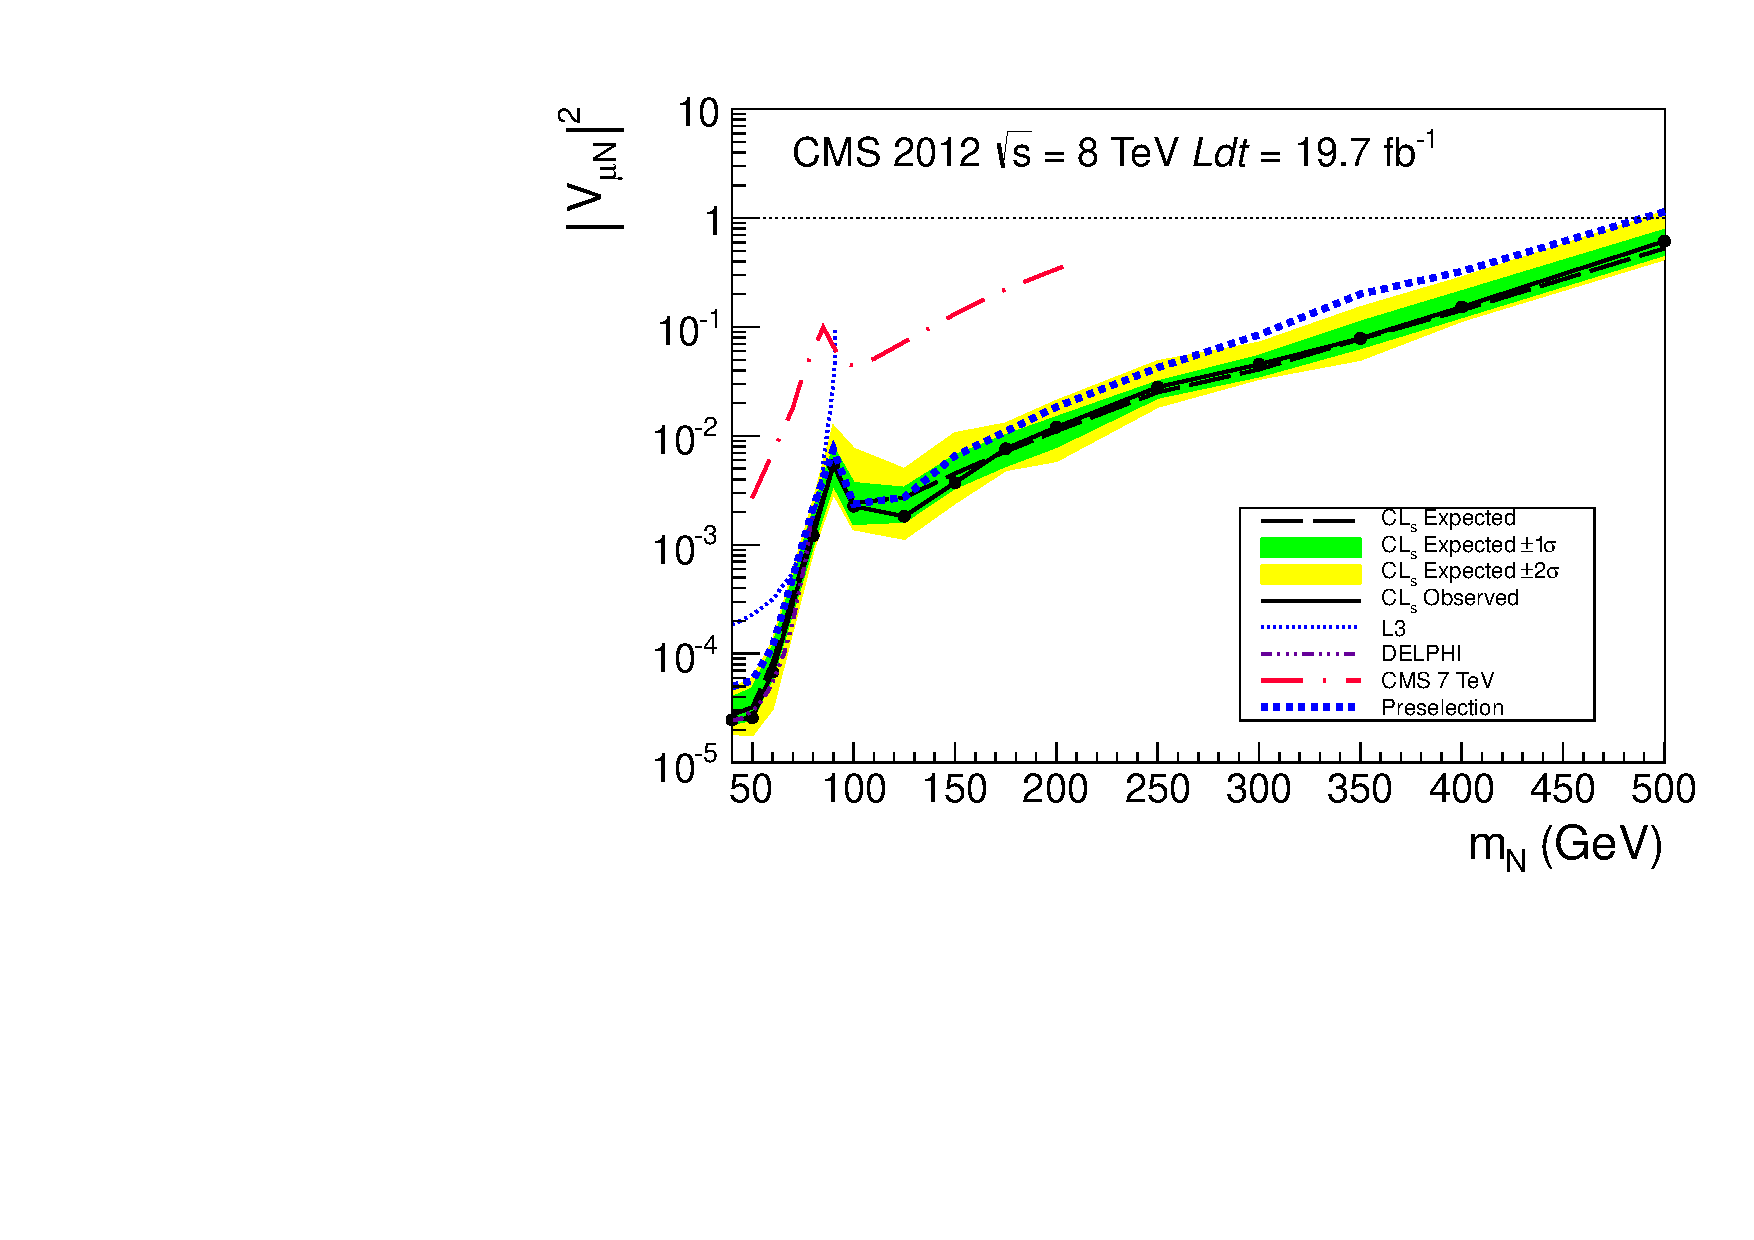
\includegraphics[scale=0.75]{figures/Ch_3_Results/exclusion_mm.pdf}
% 		\par\end{centering}
% 		\caption[Exclusion region of the HMN mixing element vs. mass.]{\label{fig:exclusion}Exclusion region of the HMN mixing element vs. mass.  The black hashed line is the expected limit for Standard Model processes, with no HMN.  The black solid line shows the exclusion set by this analysis.  The blue dotted line shows where the limits would be set if no selection optimization was performed on each mass point and only preselection cuts were used.  The remaining lines compare previous search limits.}
% 	\end{figure}
% 	%%%%%%%%%%%%%%%%%%%%%%%%%%%%%%%%%%%%%%%%%%%%%%%%%%%%%%%%%%%%%%%%%%%%%%%%%%%%%%%%%%%

% 	%%%%%%%%%%%%%%%%%%%%%%%%%%%%%%%%%%% Exclusion Plot %%%%%%%%%%%%%%%%%%%%%%%%%%%%%%%%%%%%%%%%
% 	\begin{figure}
% 		\begin{centering}
% 			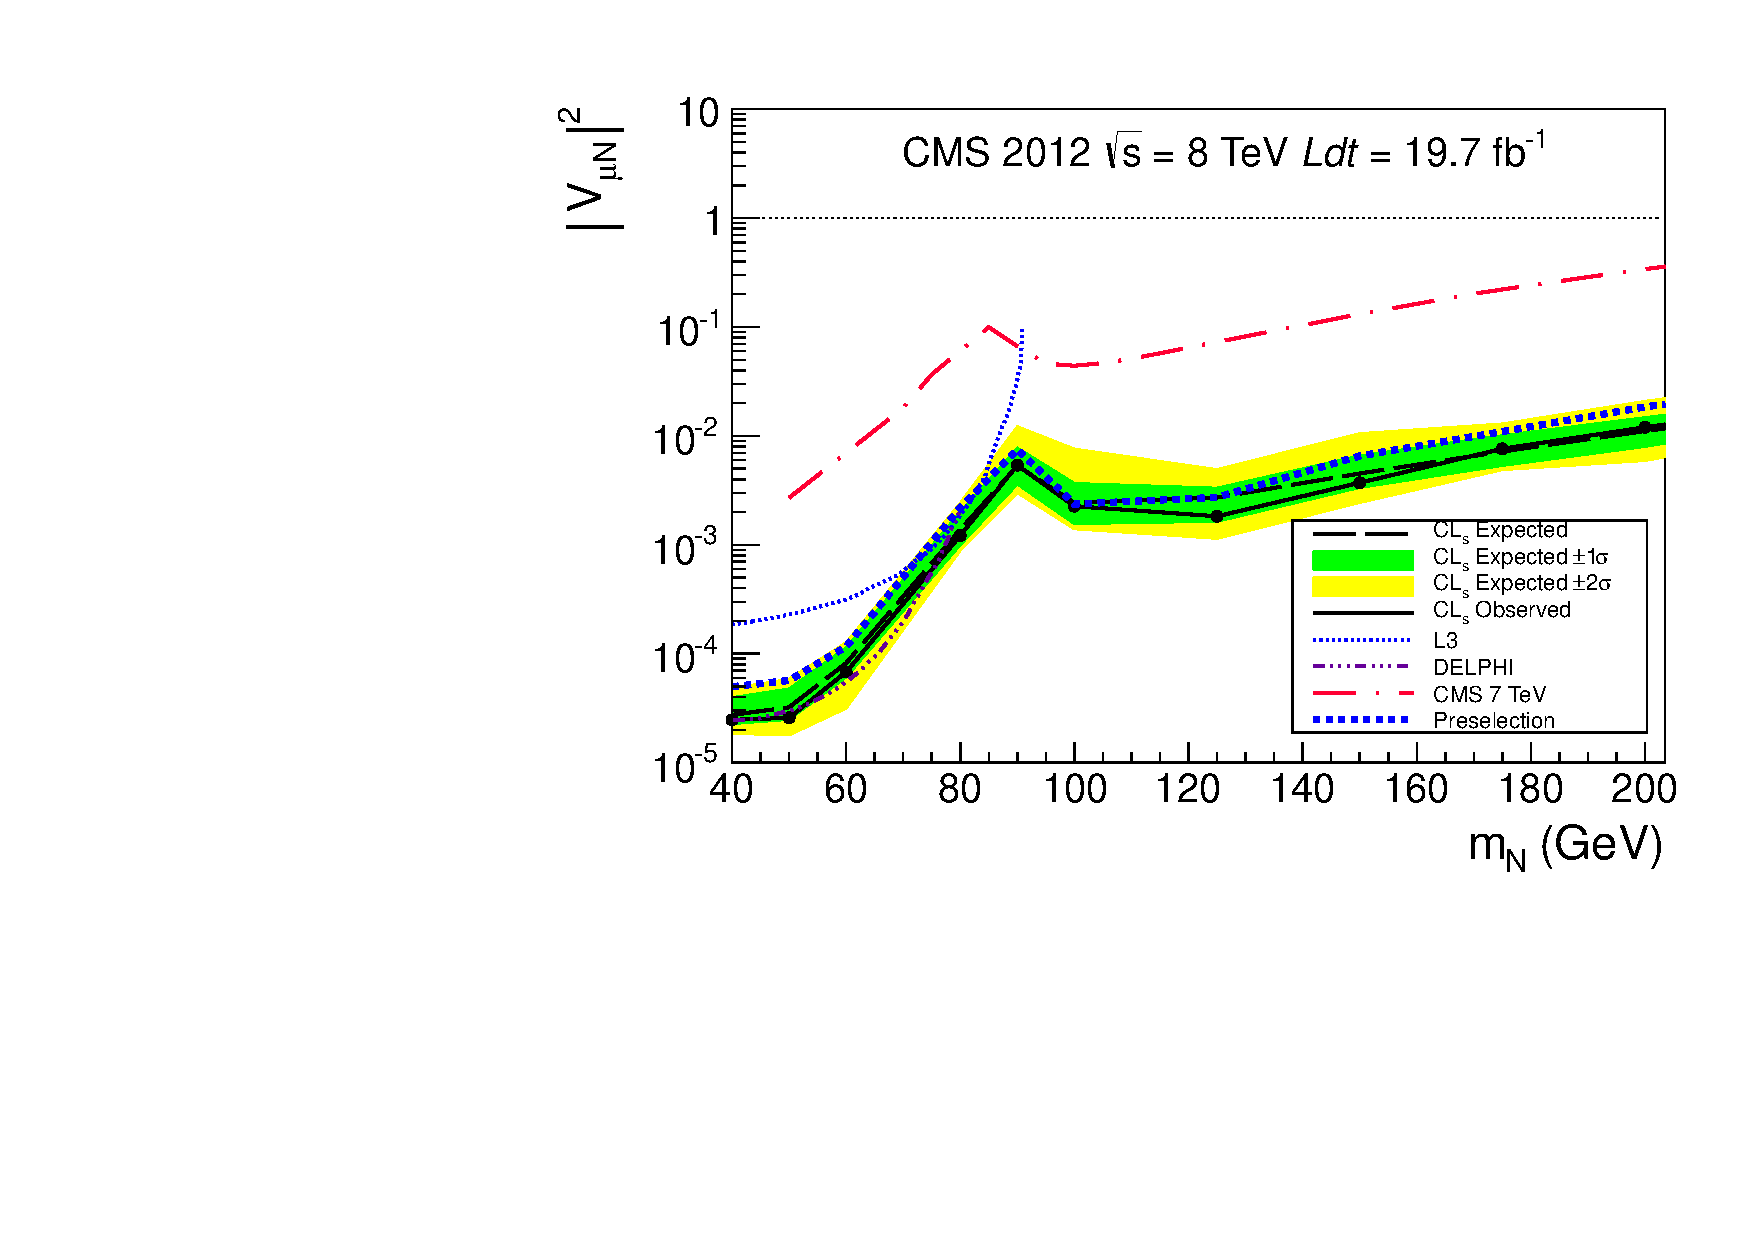
\includegraphics[scale=0.75]{figures/Ch_3_Results/exclusion_mm_zoom.pdf}
% 		\par\end{centering}
% 		\caption[Zoom of Figure \ref{fig:exclusion} at low mass.]{\label{fig:exclusionZoom}Zoom of Figure \ref{fig:exclusion} at low mass.}
% 	\end{figure}
% 	%%%%%%%%%%%%%%%%%%%%%%%%%%%%%%%%%%%%%%%%%%%%%%%%%%%%%%%%%%%%%%%%%%%%%%%%%%%%%%%%%%%


% \section{Future Prospects}
% 	With the LHC planning to start Run 2015 at a higher collision energy, with higher luminosity, the prospects for improving the exclusion at low HMN mass is not likely, due to the increased pileup, obfuscating the low p$_\text{T}$ muons produced by a low mass HMN.  However, there is already good exclusion at low mass, and the HMN mass is thought to exist most likely at a much higher mass than what is currently able to be observed.  An analysis of run 2015 data will be able to set exclusions at a much higher mass range, and there is always the possibility of discovery.




% %%% HF Lowering %%%
% \begin{figure}[H]
% 	\begin{center}
% 		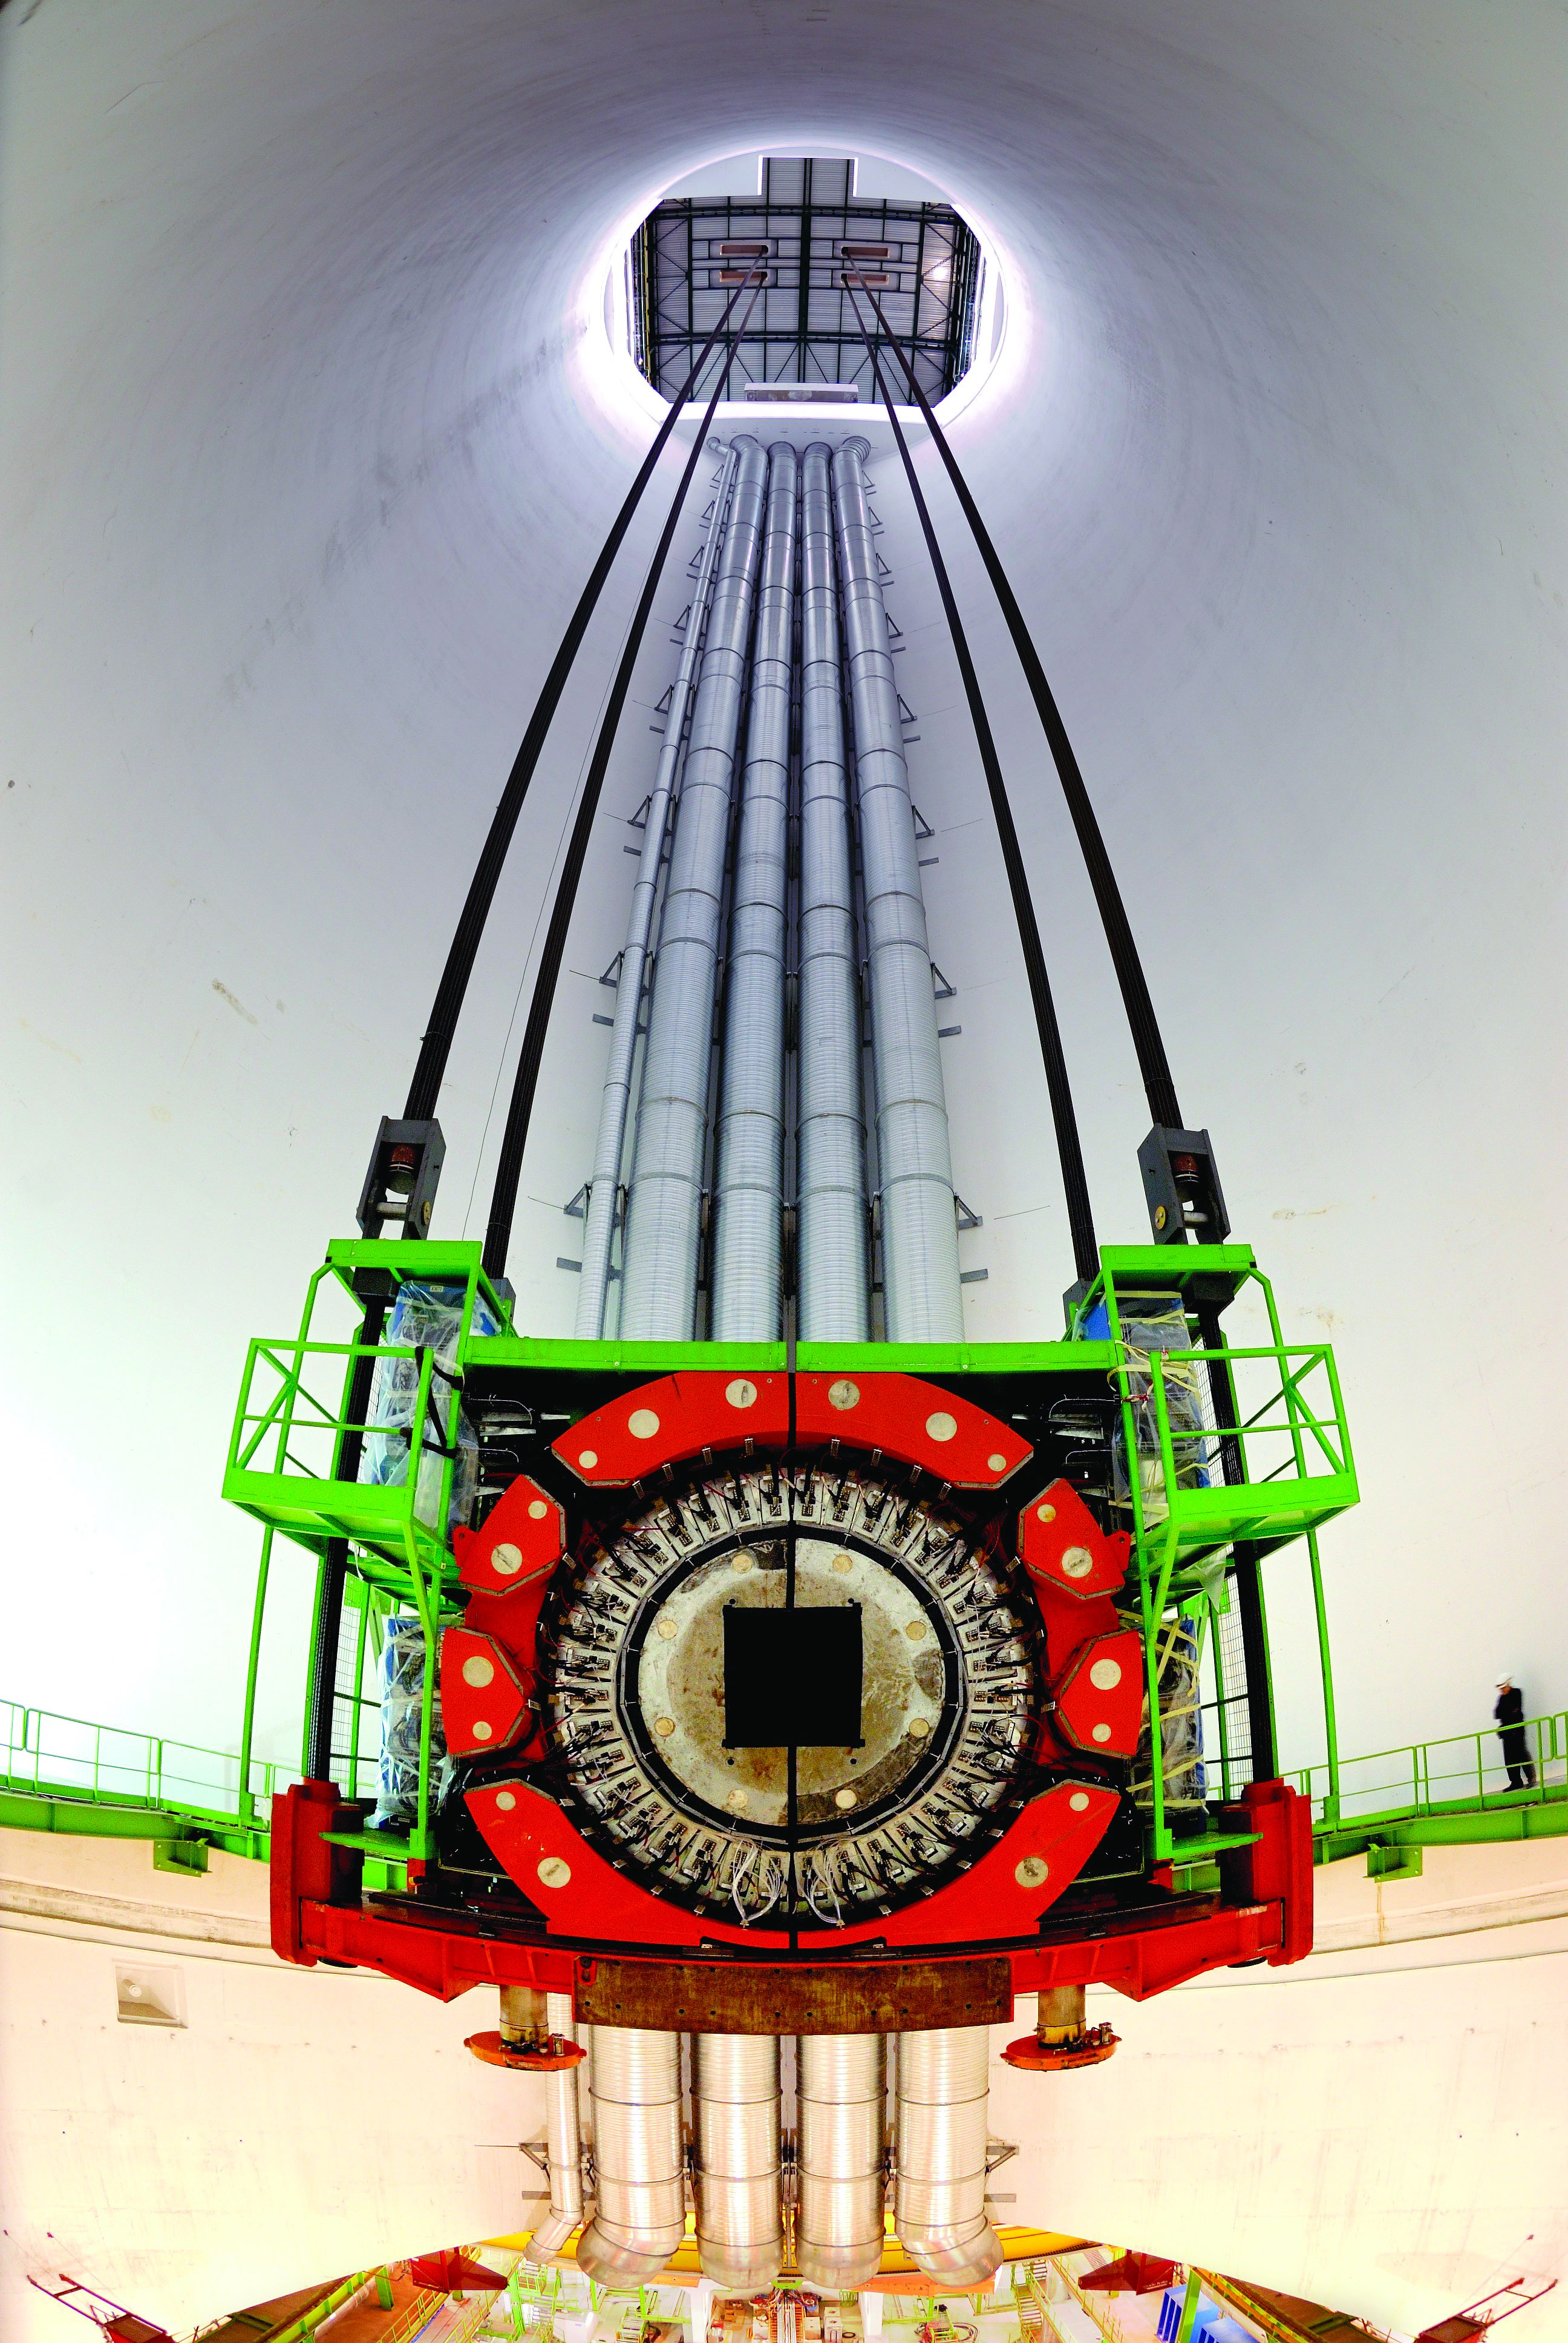
\includegraphics[width=0.98\textwidth]{figures/Ch_4_raddam/HFLowering.jpg}
% 		\caption{HF Lowering.}
% 		\label{fig:hflowering}
% 	\end{center}
% \end{figure}



